%% Master Thesis Template
%% Please update the specification through this link: https://daim.idi.ntnu.no/howto_thesis_submission.pdf

\documentclass[pdftex,10pt,b5paper,twoside]{book}


%========================================================================
%   PACKAGES
%========================================================================

\usepackage[lmargin=25mm,rmargin=25mm,tmargin=27mm,bmargin=30mm]{geometry}
\usepackage{setspace}
\usepackage{graphicx}
\usepackage{amssymb}
\usepackage{mathrsfs}
\usepackage{amsthm}
\usepackage{amsmath}
\usepackage{color}
\usepackage[Lenny]{fncychap}
\usepackage[pdftex,bookmarks=true]{hyperref}
\hypersetup{
    colorlinks,%
    citecolor=black,%
    filecolor=black,%
    linkcolor=black,%
    urlcolor=black
}
\usepackage[font=small,labelfont=bf,list=true,listformat=simple]{caption}
\usepackage{fancyhdr}
\usepackage{times}
\usepackage{float}

\usepackage[
backend=biber,
natbib=true,
citestyle=authoryear
]{biblatex}

\usepackage{listings} % For code listings
\usepackage{chngcntr} % To change counters

\usepackage[utf8]{inputenc} % utf-8 support

\usepackage{tocbibind} % Adding toc, lists of tables, and figures to toc
\usepackage[acronym,nonumberlist,toc]{glossaries} % Abbreviations

\usepackage{minted} % For nice appendix page
\usepackage[toc, page]{appendix} % For nice appendix page

\usepackage{tabulary} % Tabulary

\usepackage[nodayofweek,level]{datetime} % To print dates
\usepackage{mathtools} % Math tools
\usepackage{pifont} % For extra symbols

% For landscape
\usepackage{pdflscape}

\usepackage{algorithm2e} % Pseudo code

\usepackage{tikz} % To draw figures

\usepackage[inline]{enumitem} % To remove item step in itemize

\usepackage{xcolor, colortbl} % For extra color support

\usepackage{placeins} % To make sure figures stays in their section

\usepackage[noabbrev,capitalize]{cleveref} % For clever references


%========================================================================
%   CONFIGURATION
%========================================================================

\restylefloat{figure}


\newcommand{\HRule}{\rule{\linewidth}{0.5mm}}


\renewcommand{\chaptermark}[1]{\markboth{\chaptername\ \thechapter.\ #1}{}}
\renewcommand{\sectionmark}[1]{\markright{\thesection\ #1}}
\renewcommand{\headrulewidth}{0.1ex}
\renewcommand{\footrulewidth}{0.1ex}


\fancypagestyle{plain}{\fancyhf{}\fancyfoot[LE,RO]{\thepage}\renewcommand{\headrulewidth}{0ex}}


% Document information
\title{Beating the bookmakers}
\author{Simon Borøy-Johnsen}


% Make sure floats are placed correctly
\let\Oldsection\section
\renewcommand{\section}{\FloatBarrier\Oldsection}

\let\Oldsubsection\subsection
\renewcommand{\subsection}{\FloatBarrier\Oldsubsection}

\let\Oldsubsubsection\subsubsection
\renewcommand{\subsubsection}{\FloatBarrier\Oldsubsubsection}

\floatplacement{figure}{ht}
\floatplacement{table}{ht}


% Rename appendix chapter to appendix
\crefname{appendix}{Appendix}{Appendices}


% Custom date
\newdateformat{monthyear}{\monthname[\THEMONTH] \THEYEAR}


% Rename lists
\renewcommand*\contentsname{Table of Contents}
\renewcommand*{\acronymname}{List of Abbreviations}
\renewcommand*{\lstlistlistingname}{List of Listings}


% Add list of listings to toc
\renewcommand{\lstlistoflistings}{\begingroup\tocfile{\lstlistlistingname}{lol}\endgroup}


% Generate abbreviations
%\newacronym{}{}{}
\newacronym{ann}{ANN}{artificial neural network}
\newacronym{fnn}{FNN}{feedforward neural network}
\newacronym{rnn}{RNN}{recurrent neural network}
\newacronym{cnn}{CNN}{convolutional neural network}

\newacronym{knn}{kNN}{k-nearest neighbor}
\newacronym{svm}{SVM}{support vector machine}

\newacronym{mse}{MSE}{mean squared error}
\newacronym{mae}{MAE}{mean absolute error}

\newacronym{html}{HTML}{HyperText Markup Language}
\makeglossaries


% Add prefix to figures
\graphicspath{ {figures/} }


% Adding internal counters to figures and tables
\counterwithin{figure}{section}
\counterwithin{table}{section}


% Add bibliography
\addbibresource{references.bib}


% Set code listings style
\lstset{basicstyle=\ttfamily}
\lstset{breaklines}


% Add bozes around algorithms
\RestyleAlgo{boxruled}


% Set numbering depth
\setcounter{tocdepth}{1} % Includes up to sections in the table of contents
\setcounter{secnumdepth}{2} % Numbers up to sub-subsections


% Check-mark and cross
\newcommand{\cmark}{\ding{51}}
\newcommand{\xmark}{\ding{55}}


% Other custom commands
\newcommand{\whoscoredplain}{www.whoscored.com}
\newcommand{\whoscored}{\textbf{\whoscoredplain}}
\newcommand{\whoscoredurl}[1]{\url{\whoscoredplain#1}}


% Nicer parentheses in equations
\delimitershortfall = -1pt


% Best configuration color in results
\definecolor{correct}{rgb}{0.56, 0.93, 0.56}


% For JavaScript listings
\definecolor{lightgray}{rgb}{.9,.9,.9}
\definecolor{darkgray}{rgb}{.4,.4,.4}
\definecolor{purple}{rgb}{0.65, 0.12, 0.82}

\lstdefinelanguage{JavaScript}{
  keywords={break, case, catch, continue, debugger, default, delete, do, else, false, finally, for, function, if, in, instanceof, new, null, return, switch, this, throw, true, try, typeof, var, void, while, with},
  morecomment=[l]{//},
  morecomment=[s]{/*}{*/},
  morestring=[b]',
  morestring=[b]",
  ndkeywords={class, export, boolean, throw, implements, import, this},
  keywordstyle=\color{blue}\bfseries,
  ndkeywordstyle=\color{darkgray}\bfseries,
  identifierstyle=\color{black},
  commentstyle=\color{purple}\ttfamily,
  stringstyle=\color{red}\ttfamily,
  sensitive=true
}

\lstset{
   language=JavaScript,
   backgroundcolor=\color{lightgray},
   extendedchars=true,
   basicstyle=\footnotesize\ttfamily,
   showstringspaces=false,
   showspaces=false,
   numbers=left,
   numberstyle=\footnotesize,
   numbersep=9pt,
   tabsize=2,
   breaklines=true,
   showtabs=false,
   captionpos=b
}


% Setting up tikz

\usetikzlibrary{positioning}

\tikzset{%
  every neuron/.style={
    circle,
    draw,
    minimum size=17pt
  },
  neuron missing/.style={
    draw=none, 
    scale=2,
    text height=0.333cm,
    execute at begin node=\color{black}$\vdots$
  },
}


%========================================================================
%   DOCUMENT START
%========================================================================

\begin{document}


% Set page style for summary, preface, and contents
\pagenumbering{roman}
\pagestyle{fancy}
\fancyhf{}
\renewcommand{\chaptermark}[1]{\markboth{\chaptername\ \thechapter.\ #1}{}}
\renewcommand{\sectionmark}[1]{\markright{\thesection\ #1}}
\renewcommand{\headrulewidth}{0.1ex}
\renewcommand{\footrulewidth}{0.1ex}
\fancyfoot[LE,RO]{\thepage}
\fancypagestyle{plain}{\fancyhf{}\fancyfoot[LE,RO]{\thepage}\renewcommand{\headrulewidth}{0ex}}


%========================================================================
%   ABSTRACT
%========================================================================

\section*{\Huge Summary}
\addcontentsline{toc}{chapter}{Summary}
$\\[0.5cm]$

\glspl{ann} have throughout the years been used for several purposes. Problems spanning from image classification to text generation have all been subject to \glspl{ann}.

In this report, \glspl{ann} were used in order to predict the outcomes of football matches. Using data from the football statistics web site \whoscored, \glspl{ann} were constructed in order to predict the outcomes of matches from two successive seasons of the English Premier League. The predictions were then used to decide whether or not to place bets on the outcomes, in an effort to generate a profit.

Several \glspl{ann} were constructed, utilizing data sources from player ratings to team characteristics. The networks were trained using simple back-propagation training. The predictions were then used together with odds from seven international bookmakers, trying to generate a profit from betting. Different money management (betting) strategies were applied, in order to highlight the importance of choosing correct bet sizes.

The results show that simple assumptions show promising results when predicting the outcome of a football match. The results also show that \glspl{ann} can indeed beat bookmakers in their own game, and gain a profit from football betting.

The report ends with the author's thoughts on how to further improve the profitability of the presented models.

\cleardoublepage


%========================================================================
%   SAMMENDRAG
%========================================================================

\section*{\Huge Sammendrag}
\addcontentsline{toc}{chapter}{Sammendrag}
$\\[0.5cm]$

Nevrale nettverk har i en årrekke blitt brukt til flere forskjellige formål. Alt fra bildeklassifisering til tekstgenerering har blitt utprøvd ved hjelp av nevrale nettverk.
 
I denne rapporten ble nevrale nettverk brukt til å predikere resultatene til fotballkamper. Ved å bruke data fra fotballstatistikk-nettstedet \whoscored\ , ble nevrale nettverk brukt for å predikere resultatene for kamper fra to sammenhengende sesonger av engelske Premier League. Prediksjonene ble deretter brukt til å avgjøre hvorvidt man skulle sette penger på resultatene, i et forsøk på å generere profitt.
 
Flere nevrale nettverk ble konstruert. Nettverkene brukte datakilder fra spillerrangeringer til lag-karakteristikker. De ble trent ved hjelp av simpel “backpropagation”-trening. Prediksjonene ble brukt sammen med odds fra syv internasjonale tippeselskap, i et forsøk på å generere profitt fra tipping. Forskjellige pengestyrings-strategier ble utprøvd, for å fremheve viktigheten av å velge riktige innsatsstørrelser.
 
Resultatene viser at enkle antagelser kan være nok for å nøyaktig predikere resultatene for fotballkamper. Resultatene viser også at nevrale nettverk kan brukes til å slå tippeselskapene i sitt eget spill: å tjene penger på fotballtipping.
 
Rapporten avsluttes med forfatterens tanker om hvordan å forbedre de presenterte resultatene ytterlige.

\cleardoublepage


%========================================================================
%   PREFACE
%========================================================================

\section*{\Huge Preface}
\addcontentsline{toc}{chapter}{Preface}
$\\[0.5cm]$

This master thesis has been carried out at the \gls{idi} at \gls{ntnu}. The thesis was written in order to fulfill the graduation requirements of the Computer Science program at \gls{ntnu}. I was engaged in researching and writing this study from August 2016 to June 2017.

I would like to thank all the people who have helped me carry out this thesis. Thanks to my supervisor, Helge Langseth, for his indispensable guidance and sincere opinions throughout this work. I would also like to thank two of my fellow students, Simen Selseng and Magnus Gundersen, for keeping me company while writing this thesis. Without them, I would not have made it through the long days at the study hall.

Last but not least, I would like to thank my fiancee, Marianne Gilje, for inspiring and supporting me throughout my studies and our eight years together.

I hope you enjoy your reading.

$\\[0.5cm]$

\noindent \textbf{Simon Borøy-Johnsen}

\noindent Trondheim, \monthyear{\today}

\cleardoublepage


%========================================================================
%   TABLE OF CONTENTS, FIGURES, TABLES, ABBREVIATIONS
%========================================================================

\pdfbookmark[1]{\contentsname}{toc}

\tableofcontents
\clearpage

% Roman page numbering
\pagenumbering{roman}

\listoffigures % List of figures
\listoftables % List of tables
\printacronyms[title=Abbreviations] % List of abbreviations

\clearpage


% Reset page style
\pagenumbering{arabic}
\pagestyle{fancy}
\fancyhf{}
\renewcommand{\chaptermark}[1]{\markboth{\chaptername\ \thechapter.\ #1}{}}
\renewcommand{\sectionmark}[1]{\markright{\thesection\ #1}}
\renewcommand{\headrulewidth}{0.1ex}
\renewcommand{\footrulewidth}{0.1ex}
\fancyfoot[LE,RO]{\thepage}
\fancyhead[LE]{\leftmark}
\fancyhead[RO]{\rightmark}
\fancypagestyle{plain}{\fancyhf{}\fancyfoot[LE,RO]{\thepage}\renewcommand{\headrulewidth}{0ex}}


%========================================================================
%   CHAPTER: INTRODUCTION
%========================================================================

\chapter{Introduction}
\label{chp:introduction}
Association football (hereafter referred to as \textbf{football}) is one of the most popular sports in the world. The sport is played by millions of people all over the world, both for fun and professionally. Even more people enjoy watching the sport being played by professionals, in both national and international competitions \citep{bib:fifa}.

Several bookmakers all around the world allow placing bets on almost every aspect of a match: from the final outcome to which team will be awarded the next throw-in. Predicting the outcomes of football matches is a difficult task. The complexity of the sport, and the vast amount of variables affecting the outcome, increase the difficulty. Injuries, the physical and psychological shape of the players, referees and more; all contribute to the final outcome of a match.

\gls{ai} is as popular as ever, with tech giants such as Google and Microsoft pouring millions of dollars into acquiring \gls{ai} companies (\citet{bib:deepmind}, \citet{bib:maluuba}). This report will explore how \gls{ai}, more specifically \glspl{ann}, can be used for predicting the outcomes of football matches. The prediction models produced will be tested in a real-life simulation, trying to beat the bookmakers in their own game: by profiting from betting.
\section{Research questions}
\section{Report outline}


%========================================================================
%   CHAPTER: BACKGROUND
%========================================================================

\chapter{Background}
\label{chp:background}
This chapter presents the background research conducted before starting the work in this report. \cref{sec:background-models}, \cref{sec:background-variables}, and \cref{sec:background-betting} were part of a specialization project done at \gls{ntnu} \citep{bib:boroy-johnsen-2016}.
\section{Models used for predicting outcomes of football matches}

Already in 1982, \citeauthor{bib:maher-1982} presented a model for predicting the outcomes of football matches. Earlier studies in the field of football match results predictions used the negative binomial distribution to model the number of goals a given team will score during a given match. The earlier studies had rejected the Poisson model for predicting football results, stating that "chance does dominate the game" \citep{bib:maher-1982}. This assumption was shown wrong by \citet{bib:hill-1974}. Experts are able to accurately predict the final league standings before the league even start. According to \citet{bib:maher-1982}, this indicates that chance may play a considerable part in the results of a match, but differences in teams strengths and skills dominate in the long run.

A team's strength is usually divided into two separate strengths; attacking and defensive strengths. The attacking strength of a team represents the team's ability to score goals. The defensive strength of a team represents the team's ability to avoid conceding goals.

\subsection{The Poisson distribution}

\citet{bib:maher-1982} laid the foundation for several later prediction models when he presented his Poisson distribution model for predicting the number of goals scored by the the competing teams during a match. His model is based on the following assumption; each time a team has possession of the ball, there is an opportunity to attack, with the probability \textit{p} of scoring a goal. There are \textit{n} attacks during a match. If \textit{p} is constant, and the attacks are independent, the number of goals can be approximated using the Poisson distribution. \citet{bib:maher-1982} assumed that if team \textit{i} is playing at home against team \textit{j}, and the final scoreline is $(x_{ij}, y_{ij})$, then the final scoreline can be modelled using \referequation{eq:maher-model}.
\begin{equation}
    \begin{aligned}
        X_{ij} \sim P(\alpha_{i}\beta_{j}) \\
        Y_{ij} \sim P(\gamma_{i}\delta_{j})
    \end{aligned}
    \label{eq:maher-model}
\end{equation}
\citet{bib:maher-1982} described that the variables represent different aspects of the match. A summary is given in \refertable{tab:maher-model-description}.
\begin{table}[H]
    \centering
    \noindent\begin{tabulary}{\textwidth}{C | L}
        \textbf{Variable}   & \textbf{What it represents} \\\hline
        $\alpha_{i}$        & The strength of team \textit{i}'s attack when playing at home \\
        $\beta_{j}$          & The weakness of team \textit{j}'s defence when playing away \\
        $\gamma_{i}$        & The weakness of team \textit{i}'s defence when playing at home \\
        $\delta_{j}$        & The strength of team \textit{j}'s attack when playing away \\
    \end{tabulary}
    \caption{The variables in the model of \citet{bib:maher-1982}.}
    \label{tab:maher-model-description}
\end{table}
The variables are based on the number of goals scored and conceded in the teams' earlier matches.

\subsubsection{Double Poisson distribution}

In the initial model of \citet{bib:maher-1982}, $X_{ij}$  and $Y_{ij}$ are assumed to be independent, "representing separate “games” at the two ends of the pitch". This is known as the double Poisson distribution.

Because of the independence, $\alpha$ and $\beta$ can be estimated for $x$ alone, whilst $\gamma$ and $\delta$ can be estimated from $y$ alone \citep{bib:maher-1982}. The log likelihood function for the home team's score can therefore be expressed as in \referequation{eq:maher-log-likelihood}.
\begin{equation}
    log\ L(\alpha, \beta) = \sum_{i} \sum_{j \neq i} (-\alpha_{i} \beta_{j} + x_{ij}\ log(\alpha_{i}\beta_{j}) - log(x_{ij}!))
    \label{eq:maher-log-likelihood}
\end{equation}
Further, the maximum likelihood estimates, $\hat{\alpha}, \hat{\beta}$ can be shown to satisfy \referequation{eq:maher-maximum-likelihood-estimates} \citep{bib:maher-1982}.
\begin{equation}
    \begin{aligned}
        \hat{\alpha_{i}} = \frac{\sum_{j \neq i} x_{ij}}{\sum_{j \neq i} \hat{\beta_{j}}} \\
        \hat{\beta_{j}} = \frac{\sum_{i \neq j} x_{ij}}{\sum_{i \neq j} \hat{\alpha_{i}}}
    \end{aligned}
    \label{eq:maher-maximum-likelihood-estimates}
\end{equation}
To determine the maximum likelihood estimates, \citet{bib:maher-1982} used the Newton-Raphson method. The similar was done for $\hat{\gamma}$ and $\hat{\delta}$. The determined estimates show the effects of the home ground advantage, as each team's attacking strength is significantly reduced when playing away \citep{bib:maher-1982}.

When evaluating his model, \citet{bib:maher-1982} used data from the four English Football League divisions for three consecutive years (1973-1975). \referfigure{fig:app-maher-strengths} shows the calculated team strengths for all teams in the English Division 1 1971-1972. \citet{bib:maher-1982} raised the question of whether using four different parameters for each team is really necessary. Using maximum likelihood estimates, \citet{bib:maher-1982} showed that the relative strengths of teams' attack and defense are the same whether playing at home or away, and that only $\alpha$ and $\beta$ are needed in order to make reasonable predictions. \citet{bib:maher-1982} then looked at the frequencies of goal scores scored in the English Division 1 over the three seasons. The results are shown in \referfigure{fig:app-maher-double-frequencies}. The model seems to underestimate the number of occasions where one and two goals are scored, while overestimating the number of times no or $\geq 4$ goals are scored \citep{bib:maher-1982}.

Even though the model has shown promising results, the assumptions behind it are not realistic \citep{bib:maher-1982}. \citet{bib:dixon-robinson-1998} showed how \textit{p} changes throughout the lifespan of a match. The scoring rate seems to increase throughout the game. \citet{bib:dixon-robinson-1998} pondered that the teams fatigue near the end of the match, making defensive mistakes, which in turn lead to goals. They also showed how the scoring rates are dependent on the current score. A lead to the home team tends to decrease their scoring rate, whilst increasing the scoring rate of the opposing team. A lead for the away team tends to increase the scoring rate of both teams.

\subsubsection{Bivariate Poisson distribution}

To accommodate the over-simplification of his model, \citet{bib:maher-1982} used the available data to create an improved, bivariate Poisson distribution model. In the new model, the marginal distributions are still Poisson with the same means as before, but a correlation factor, $\varrho$, is added between the scores. The new model can be thought of as considering the difference in the number of goals scored, $Z_{ij} = X_{ij} - Y_{ij}$, resulting in a model with two dependent parts \citep{bib:maher-1982}. One way to think of the bivariate Poisson distribution, according to \citet{bib:maher-1982}, is that
\begin{equation*}
    X_{ij} = U_{ij} + W_{ij} \quad \text{and} \quad Y_{ij} = V_{ij} + W_{ij},
\end{equation*}
where $U_{ij}$, $V_{ij}$ and $W_{ij}$ are independent Poisson with means $(\mu_{ij} - \eta_{ij})$, $(\lambda_{ij} - \eta_{ij})$ and $\eta_{ij}$ respectively, with $\eta_{ij}$ being the co-variance between $X_{ij}$ and $Y_{ij}$. \citet{bib:maher-1982} experimented with different values for $\varrho$, and a value of $0.2$ yielded the best results. The bivariate version of his model improved the results considerably, compared to the initial model. \referfigure{fig:app-maher-bivariate-frequencies} shows the different frequencies for $Z_{ij}$ when applying the model to the English Division 1 1971-1972. One issue present in both the initial and improved models is the tendency to underestimate the number of drawn matches.

It is hard to say whether there is any correlation between the number of goals scored by each competing team. The question has been brought up in several studies. The assumption is, according to \citet{bib:maher-1982}, too simple to model reality. \citet{bib:karlis-ntzoufras-2003} argued that since two teams interact with each other during a match, the number of goals scored by each team are correlated. A change of style in play from one team will in turn change the probabilities of scoring a goal for both teams \citep{bib:karlis-ntzoufras-2003}. They supported their statements by analyzing data from the Champions League 2000-2001. \citet{bib:mchale-scarf-2007}, on the other hand, found little to no evidence of any correlation between the number of goals scored by the opposing teams. They used data from the English Premier League 2003-2006.

\citet{bib:karlis-ntzoufras-2003} built upon the model of \citet{bib:maher-1982}. They also used the bivariate Poisson distribution in their model. \citet{bib:karlis-ntzoufras-2003} modelled the number of goals scored in a match somewhat different from \citet{bib:maher-1982}. Instead of adding the correlation factor separately from the distribution, \citet{bib:karlis-ntzoufras-2003} added it to the distribution itself, resulting in a model of the form $(X_{ij}, Y_{ij}) \sim BP(\lambda_{i}, \lambda_{j}, \varrho)$, where
\begin{equation}
    \begin{aligned}
        log(\lambda_{i}) = \mu + H + \alpha_{i} + \beta_{j}
        \quad \text{and} \quad
        log(\lambda_{j}) = \mu + \alpha_{j} + \beta_{i}.
    \end{aligned}
    \label{eq:karlis-ntzoufras-model}
\end{equation}
$\lambda_{i}$ and $\lambda_{j}$ represent the expected number of goals scored for the home and away teams, respectively. $\varrho$ is the correlation factor, $\mu$ is a constant parameter, and $H$ is the home team effect parameter. $\alpha_{k}$ and $\beta_{i}$ represent the attacking and defensive abilities of team $k$, like in the model of \citet{bib:maher-1982}. $\mu$ represents the average number of goals scored per team when two teams of similar strengths play against each other.

Increasing the correlation between the number of goals scored improved the accuracy in prediction of draw games. \citet{bib:karlis-ntzoufras-2003} further improved their model by inflating the probability of drawn games. They stated that inflating the probability corrected a possible overdispersion of results. \referfigure{fig:app-karlis-ntzoufras-2003-results} shows the estimates for different versions of their model. Model 8, the diagonal inflated bivariate Poisson distributed model, shows the most promising results.

The model of \citet{bib:koopman-lit-2015} is also based on the bivariate Poisson distribution of \citet{bib:maher-1982}. Their model is similar to that of \citet{bib:karlis-ntzoufras-2003};
\begin{equation*}
    (X_{ij}, Y_{ij}) \sim BP(\lambda_{i}, \lambda_{j}, \varrho),
\end{equation*}
where $\lambda_{i}$ and $\lambda_{j}$ are the intensity coefficients for $X$ and $Y$, and $\gamma$ is the coefficient that measures the dependence between $X_{ij}$ and $Y_{ij}$. $\lambda_{i}$ and $\lambda_{j}$ are allowed to vary over time. The intensities are then specified as
\begin{equation*}
    \begin{aligned}
        \lambda_{i, ijt} = exp(H + \alpha_{it} + \beta_{jt}) \\
        \lambda_{j, ijt} = exp(\alpha_{jt} + \beta_{it}),
    \end{aligned}
\end{equation*}
where $H$ is the home ground advantage coefficient and $\alpha_{kt}$ and $\beta_{kt}$ the attacking and defensive strengths of team $k$ in game week $t$. The attacking and defensive strengths are specified in \referequation{eq:koopman-lit-team-strengths},
\begin{equation}
    \begin{aligned}
        \alpha_{it} = \mu_{\alpha, i}  + \phi_{\alpha, i}\ \alpha_{i, t-1} + \eta_{\alpha, it} \\
        \beta_{it} = \mu_{\beta, i}  + \phi_{\beta, i} \ \beta_{i, t-1} + \eta_{\beta, it}
    \end{aligned}
    \label{eq:koopman-lit-team-strengths}
\end{equation}
where $\mu_{\alpha, i}$ and $\mu_{\beta, i}$ are unknown constants, $\phi_{\alpha, i}$ and $\phi_{\beta, i}$ are auto-regressive coefficients, and $\eta_{\alpha, it}$ and $\eta_{\beta, it}$ are normally distributed independent error terms. $\alpha_{it}$ and $\beta_{it}$ are determined using the maximum likelihood estimator.

\citet{bib:koopman-lit-2015} applied their model in a betting setting. They used their predictions in combination with odds published at \citet{bib:football-data} for the English Premier League 2010-2012. During the evaluation, they used the Fixed bet strategy explained in \refersection{sec:betting-strategies}, with a variable threshold $\tau$. \referfigure{fig:app-koopman-lit-threshold-levels} shows the effect $\tau$ has on the profitability of their system. With $\tau > 0.12$, the system is able to systematically gain a profit.


\subsubsection{Altered Poisson distribution models}

\citet{bib:dixon-coles-1997} used the initial model of \citet{bib:maher-1982} as basis for their model, with a small modification. The modified model included the home ground parameter, and can be seen in \referequation{eq:dixon-coles-model}.
\begin{equation}
    \begin{aligned}
        X_{ij} \sim Poisson(\alpha_{i} \beta_{j} H) \\
        Y_{ij} \sim Poisson(\alpha_{j} \beta_{i}),
    \end{aligned}
    \label{eq:dixon-coles-model}
\end{equation}
where $\alpha_{k}$ and $\beta_{k}$ are the attacking and defensive strengths of team $k$, and $H$ the home ground advantage parameter. To improve the accuracy for low-scoring matches, \citet{bib:dixon-coles-1997} modified their model further, adding a dependence parameter. The new model can be seen in \referequation{eq:dixon-coles-modified-model}.
\begin{equation}
    Pr(X_{ij} = x, Y_{ij} = y) = \tau_{\lambda, \mu}(x, y) \frac{\lambda^x exp(-\lambda)}{x!} \frac{\mu^y exp(-\mu)}{y!},
    \label{eq:dixon-coles-modified-model}
\end{equation}
where
\begin{equation}
    \begin{aligned}
        \lambda = \alpha_{i} \beta_{j} H \\
        \mu = \alpha_{j} \beta_{i}
    \end{aligned}
\end{equation}
and
\begin{equation}
    \tau_{\lambda, \mu}(x, y) =
    \begin{dcases}
        1 - \lambda \mu \varrho & \text{if } x = y = 0 \\
        1 + \lambda \varrho     & \text{if } x = 0, y = 1 \\
        1 + \mu \varrho         & \text{if } x = 1, y = 0 \\
        1 - \varrho             & \text{if } x = y = 1 \\
        1,                      & \text{otherwise}
    \end{dcases}.
\end{equation}
$\varrho$ is used as an dependence parameter. $\varrho = 0$ corresponds to independence. For $x \leq 1$ and $y \leq 1$, the independence distribution is altered.

Whilst the model of \citet{bib:maher-1982} incorporates static team strengths, \citet{bib:dixon-coles-1997} stated that recent results are more important than old ones to describe a team's current form. To incorporate this into their model, \citet{bib:dixon-coles-1997} scaled the contributions of older data, making more recent data more significant. They also modified their model to enable inclusion of incomplete data sets and data from different leagues.

\citet{bib:rue-salvesen-2000} also used the initial model of \citeauthor{bib:maher-1982} as base for their work. They represent the attacking and defensive strengths of team $i$ as random variables $\alpha_{i}$ and $\beta_{i}$ respectively. Higher values imply greater strengths. They also represent $\mu_{\alpha, i}$ and $\sigma^2_{\alpha, i}$ as the prior mean and variance of $\alpha_{i}$, and similar for defence. $e_{i} = (\alpha, \beta)_{i}$ represents the properties of team $i$. \citet{bib:rue-salvesen-2000} also added a psychological effect, modelling the underestimation when a superior team meets a team that is of supposed inferior quality. The psychological effect is given as
\begin{equation*}
    \Delta_{ij} = (\alpha_{i} + \beta_{i} - \alpha_{j} - \beta_{j}) / 2,
\end{equation*}
and replaces the home ground advantage. However, \citet{bib:rue-salvesen-2000} propose the home ground advantage to be part of an extended version of their model. Another change from the model of \citet{bib:maher-1982} is the addition of a time factor, used to weigh the recent results above more distant results. In addition to the added variables, \citet{bib:rue-salvesen-2000} did some extra modifications to the model of \citet{bib:maher-1982}. They assumed that some of the information from the final scoreline comes from the league itself, and not the actual result. In a league where each team on average scores 1.23 goals per match, scoring 1 goal in a match is actually below the expected number of goals. To model this, \citet{bib:rue-salvesen-2000} used a variable, called $\epsilon$, which determines how much the league average should contribute to the predicted number of goals. This can be interpreted in the sense that only $(1 - \epsilon) * 100\%$ of the "information" in a match result is informative on $e_{i}$ and $e_{j}$ \citep{bib:rue-salvesen-2000}. Through experiments, they found that $\epsilon = 0.2$ yielded the best predictive results. They also observed that as one team scored a lot of goals, the probabilities diverted from the Poisson distribution. This was "solved" by clipping the number of goals scored at 5. Any number of goals scored above 5 did not count. That is, 8-2 is treated as 5-2, and 6-5 as 5-5. \citet{bib:rue-salvesen-2000} are not sure whether this is the best approach to solving the problem with diverting probabilities. Another mentioned solution is to reduce the scoreline until one get a more common one, i.e. from 7-4 to 5-2. By doing this, the information of the final result is kept, whilst removing the extra goals that do not provide important information \citep{bib:rue-salvesen-2000}. The system of \citet{bib:rue-salvesen-2000} is modelled as a Bayesian network. They added the use of Bayesian methods to update the estimates after each new match was played, and used Markov chain Monte Carlo techniques to draw inference from the network.

\citet{bib:rue-salvesen-2000} applied their model in a betting setting, using their strategy presented in \refersection{sec:betting-strategies}. The cumulative profits for the English Premier League and Division 1 1997-1998 are shown in \referfigure{fig:app-rue-salvesen-profits}. As can be seen in the figure, the system was able to gain significant profits in both leagues, with a maximum profit of $250\%$ during the simulation. According to \citet{bib:rue-salvesen-2000}, the big spike in profits in the end of January was due to a single match, Manchester United versus Leicester City. The odds for an away-win was given at $13.8$, while the model predicted a probability of $0.184$ for the same outcome. The match ended $0-1$, resulting in a significant pay-off. In the end, the final profits were $39.6\%$ and $54.0\%$ respectively. Their system was able to win $42$ of the $112$ bets placed.

\subsubsection{Poisson difference distribution models}

In a later paper, \citet{bib:karlis-ntzoufras-2008} changed from using the bivariate Poisson distribution. They instead used the Poisson difference distribution. By doing this, they removed the effect of the correlation between the performance of the competing teams, and instead modelled the goal difference directly \citep{bib:karlis-ntzoufras-2008}. To model the goal difference, \citet{bib:karlis-ntzoufras-2008} calculated
\begin{equation*}
    Z_{ij} = X_{ij} - Y_{ij} \sim PD(\lambda_{i}, \lambda_{j}),
\end{equation*}
where $X_{ij}$ and $Y_{ij}$ are the Poisson distributions for the number of goals scored by the home team and away team, respectively. $Z_{ij}$ is then the distribution of the goal difference, and is called the Skellam's distribution (or Poisson difference distribution (PDD)) \citep{bib:karlis-ntzoufras-2008}. $\lambda_{i}$ and $\lambda_{j}$ are the model parameters, modelling the expected number of goals scored by each team, just like in \citet{bib:karlis-ntzoufras-2003}. The parameters are the same as defined in \referequation{eq:karlis-ntzoufras-model}. \citet{bib:karlis-ntzoufras-2008} imposed two constraints on the attacking and defensive strengths of the teams, as given in \referequation{eq:karlis-ntzoufras-constraints},
\begin{equation}
    \sum_{k=1}^{K} \alpha_{k} = 0 \quad \text{and} \quad \sum_{k=1}^{K} \beta_{k} = 0,
    \label{eq:karlis-ntzoufras-constraints}
\end{equation}
where $K$ is the number of competing teams. The attacking and defensive parameters can the be interpreted as the deviations from a team of moderate performance. Further, $H$ is can then be interpreted as the expected goal difference in a match between two teams of the same attacking and defensive skills \citep{bib:karlis-ntzoufras-2008}. \citet{bib:karlis-ntzoufras-2008} authors show that the marginal distributions of $X$ and $Y$ are only Poisson distributed in special cases, and are in general defined as the convolution of a Poisson random variable with another discrete random variable, thus removing a large portion of the distributional assumptions concerning the number of goals scored by each team. This is one of the reasons they proposed the use of the Poisson difference distribution \citep{bib:karlis-ntzoufras-2008}. \citet{bib:karlis-ntzoufras-2008} then proceed to use Bayesian methods in order to incorporate any available information about each game via the prior distributions. Examples of mentioned relevant information are injuries, weather conditions and the fitness of the teams. Where no information is available, \citet{bib:karlis-ntzoufras-2008} proposed to use normal prior distributions for the parameters of the model, with mean equal to zero and a large variance (for example $10^4$). This is done to express prior ignorance \citep{bib:karlis-ntzoufras-2008}. The posterior predictive distributions are calculated using the Markov chain Monte Carlo algorithm.

According to \citet{bib:shahtahmassebi-moyeed-2016}, there are numerous limitations to the before-mentioned models utilizing the Poisson distribution. They cite \citet{bib:karlis-ntzoufras-2008}, supporting the use of goal difference instead of the number of goals scored. However, they address the drawback of overestimating the number of draws in the model of \citet{bib:karlis-ntzoufras-2008}. Another issue with the PDD is an issue with the double round-robin structure of most leagues. The home ground advantage results in distributions with one or both tails being too short or too long for the distribution \citep{bib:shahtahmassebi-moyeed-2016}. To overcome the limitations of the other Poisson-based models, \citet{bib:shahtahmassebi-moyeed-2016} used the generalized Poisson difference distribution (GPDD). The GPDD function is given in \referequation{eq:gpdd-mass-function}.
\begin{equation}
    f_{GPDD}(Z = X - Y = z | \lambda_{1}, \lambda_{2}, \theta_{1}, \theta_{2}) = e^{-\lambda_{1} - \lambda_{2} - \theta_{1} z} \sum_{y=0}^{\infty} (\lambda_{1}, \theta_{1})_{z + y}\ (\lambda_{2}, \theta_{2})_{y}\ e^{-(\theta_{1} + \theta_{2})y}
    \label{eq:gpdd-mass-function}
\end{equation}
for any $z \in \mathbb{Z}$, where
\begin{equation*}
    (\lambda, \theta)_{x} = \frac{\lambda(\lambda + x \theta)^{x - 1}}{x!}.
\end{equation*}
$\lambda_{1}$ and $\theta_{1}$ refer to the positive half of the distribution, while $\lambda_{2}$ and $\theta_{2}$ refer to the negative half. The GPDD model can, just like the PDD model, be used for predicting the outcome of a match, but not the scoreline itself. The GPDD model, however, introduces more flexibility in its tails than the PDD model \citep{bib:shahtahmassebi-moyeed-2016}. To model the goal difference of a match, \citet{bib:shahtahmassebi-moyeed-2016} used the GPDD model as follows:
\begin{equation*}
    \begin{aligned}
        E(Z_{i}) = \mu_{i} = H + a_{h_{i}} - a_{v_{i}} \\
        Var(Z_{i}) = \sigma_{i}^{2} = \gamma_{1} + | a_{h_{i}} - a_{v_{i}} |,
    \end{aligned}
\end{equation*}
where $a_{h_{i}}$ and $a_{v_{i}}$ are the abilities of the home and visiting team in match $i$, $H$ is the home ground effect parameters (equal for all teams), and $\gamma_{1}$ is a positive constant for the variance. The variance is defined to increase with the difference in team abilities. \citet{bib:shahtahmassebi-moyeed-2016} imposed the constraint that all abilities sum to zero $(\sum_{k=1}^{K} a_{k} = 0)$. Furthermore, the values of $\theta_{1}$ and $\theta_{2}$ are assumed constant with respect to the team abilities. The values for $\lambda_{1}$ and $\lambda_{2}$ can be obtained using \referequation{eq:shahtahmassebi-moyeed-lambda}.
\begin{equation}
    \begin{aligned}
        \lambda_{1, i} = \frac{[(1 - \theta_{2})^{2}\ \sigma_{i}^{2} + \mu_{i}] (1 - \theta_{1})^{3}}{(1 - \theta_{1})^{2} + (1 - \theta_{2})^{2}} \\
        \lambda_{2, i} = \frac{[(1 - \theta_{1})^{2}\ \sigma_{i}^{2} + \mu_{i}] (1 - \theta_{2})^{3}}{(1 - \theta_{1})^{2} + (1 - \theta_{2})^{2}}
    \end{aligned}    
    \label{eq:shahtahmassebi-moyeed-lambda}
\end{equation}
\citet{bib:shahtahmassebi-moyeed-2016} fitted the model in a Bayesian framework in order to incorporate any available information about each game via the prior distribution. The Bayesian approach allows for predicting match outcomes via the posterior predictive distribution, as well as for producing quantitative measures relating each team's performance. To generate samples for the posterior distribution, \citet{bib:shahtahmassebi-moyeed-2016} used the Markov chain Monte Carlo random walk Metropolis-Hastings algorithm. The model presented use the previous season as a baseline for the following season's results. \citet{bib:shahtahmassebi-moyeed-2016} state that teams generally at least intend to keep their position in the table from one season to the next. It is thus, according to the authors, realistic to use information from the previous season as prior information. For teams that are promoted and playing in the league for the first time, a non-informative normal prior distribution is assigned, like the one of \citet{bib:karlis-ntzoufras-2008}. The authors explain that this is done due to the nature of a football league; each team's abilities are measured relative to other teams in the same league. \citet{bib:shahtahmassebi-moyeed-2016} mention some issues with their final model. Firstly, using the previous season as baseline for the prior distributions may not be the optimal solution, as this does not allow for time-varying team abilities \citep{bib:shahtahmassebi-moyeed-2016}. They suggest an extension of the model would be to consider a dynamic model that supports varying team abilities, as well as a varying home ground advantage effect.

\subsection{Elo rating}

The ELO rating system is a rating system developed by for calculating the relative skills of players or teams in competitor-vs-competitor games, initially developed by Appard Elo. The system was initially developed for assessing the strengths of chess players, but have since been widely adopted for use in other sports \citep{bib:chessbase-2007}. The central assumption of the ELO rating system is that the performance of a competitor (either a person or a team) is a normally distributed random variable. Elo assumed the true skill level of a competitor to be the mean of this variable, and that the true skill level changes slowly over time. The skill level of a competitor serves as the basis for the competitor's ELO rating \citep{bib:chessbase-2007}.

\citet{bib:hvattum-arntzen-2010} used the ELO rating system in their model. Based on the results of previous matches, each team is assigned an ELO rating. This rating serves as a measure of the team's current strength. It should be noted that the computations of the ELO ratings need some initial ratings to be provided for each team, and that the ratings therefore can not be expected to be reliable before a sufficient number of matches have been taken into account \citep{bib:hvattum-arntzen-2010}.

Let $\ell_{i}^{H}$ and $\ell_{i}^{A}$ be the ratings of the home and away teams before a match at time $i$. A score system is defined, where points are rewarded to the teams after each match. The points awarded for a single match sum to 1. The expected score by the home and away teams are given by $\gamma^{H}$ and $\gamma^{A}$ respectively, where
\begin{equation*}
    \gamma^{H} = \frac{1}{1 + c^{(\ell_{i}^{A} - \ell_{i}^{H}) / d}} \quad \text{and} \quad
    \gamma^{A} = 1 - \gamma^{H} = \frac{1}{1 + c^{(\ell_{i}^{H} - \ell_{i}^{A}) / d}}.
\end{equation*}
$c$ and $d$ can be interpreted as setting the scaling of the rating \citep{bib:hvattum-arntzen-2010}. To calculate the ratings, the expected scores are compared to the observed scores, $\alpha^{H}$ and $\alpha^{A}$ respectively, given by
\begin{equation*}
    \alpha^{H} =
    \begin{dcases}
        1.0     & \text{if the home team wins} \\
        0.5     & \text{if the match is drawn} \\
        0,      & \text{otherwise}
    \end{dcases}
    \quad \text{and} \quad
    \alpha^{A} = 1 - \alpha^{H}.
\end{equation*}
The rating of the home team is updated after each match according to \referequation{eq:hvattum-arntzen-rating-update}. The same is done for the away team rating.
\begin{equation}
    \ell_{i}^{H} = \ell_{i-1}^{H} + k (\alpha^{H} - \gamma^{H})
    \label{eq:hvattum-arntzen-rating-update}
\end{equation}

\citet{bib:hvattum-arntzen-2010} present two different versions of the ELO rating system. The first, referred to as the \textit{basic} ELO rating ($ELO_{b}$), set $k$ to be a constant parameter. The second, referred to as the $goal based$ ELO rating ($ELO_{g}$), replace $k$ with the expression $k = k_{0}(1 + \delta)^{\lambda}$, where $k_ {0}$ and $\lambda$ are constant parameters, and $\delta$ the absolute goal difference. The \textit{goal based} rating takes the goal difference in a match into account, rewarding a 3-0 win more strongly than a 2-1 win \citep{bib:hvattum-arntzen-2010}. According to \citet{bib:hvattum-arntzen-2010}, the values of $c$ and $d$ are not that important, as they only serve to set a scale of the ratings. Alternative values for $c$ and $d$ produce identical rating systems, but one have to set suitable values for $k$, $k_{0}$ and $\lambda$ \citep{bib:hvattum-arntzen-2010}. In their experiments, \citet{bib:hvattum-arntzen-2010} set $c=10$ and $d=400$, and calibrated the values of $k$, $k_{0}$ and $\lambda$ by minimizing the quadratic loss between the predicted values and the observed outcomes.

In order to use the ELO ratings for match prediction, \citet{bib:hvattum-arntzen-2010} make use of an ordered logit regression model \citep{bib:greene-1999}. An initial set of matches is used to compute initial ratings for all the teams in the league. A second set of matches is used to estimate the parameters of the model. The rating difference,
\begin{equation*}
    x = \ell_{i}^{H} - \ell_{i}^{A},
\end{equation*}
prior to the match serves as the covariate in the regression model. This system allows for updating both the ratings and the regression parameters, ensuring the most recent data is always utilized \citep{bib:hvattum-arntzen-2010}. 

The regression model serves as the basis for calculating the match predictions. The predictions are obtained by assigning the corresponding probability for each outcome of the match, resulting in a probability distribution for the three outcomes. \referfigure{fig:hvattum-arntzen-probabilities} shows the outcome probabilities as a function of the rating difference, given by the regression model at the end of the English Premier League 2006-2007. The home win and away win probabilities are equal when the rating difference is about -80. This shows how the model captures the home ground advantage \citep{bib:hvattum-arntzen-2010}.
\begin{figure}[H]
    \centering
    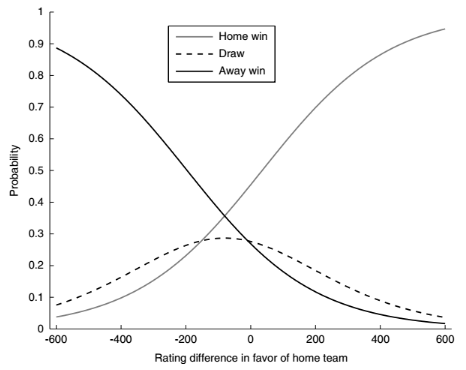
\includegraphics[width=\textwidth]{hvattum-arntzen-probabilities.png}
    \caption{Outcome probabilities as a function of rating difference (in favor of home team), given by the regression model at the end of the English Premier League season 2006/2007. Taken from \citet{bib:hvattum-arntzen-2010}.}
    \label{fig:hvattum-arntzen-probabilities}
\end{figure}

\citet{bib:hvattum-arntzen-2010} evaluated their models in a betting setting. During the evaluation, they compared their models to other prediction models. The other prediction models include naive methods like assuming uniform probability of all outcomes (UNI), and basing the probabilities of observed past frequencies (FRQ). In addition, two versions of the model presented in \citet{bib:goddard-2005} were used (GOD\textsubscript{b}, GOD\textsubscript{g}). To compare the different models, \citet{bib:hvattum-arntzen-2010} used their predictions in combination with odds collected from various bookmakers. Match data from the English Premier League seasons 1993-2008 were used. The first two seasons were used for initial calculations of the ELO ratings. The five next seasons were used for estimating the parameters in the different prediction models. Finally, the eight remaining seasons were used for actual testing. \referfigure{fig:app-hvattum-arntzen-2010-profits} shows the total return for the different models. As can be seen, none of the presented models were able to gain a profit.

\subsection{Bradley–Terry modelling}

\citet{bib:cattelan-varin-firth-2013} built a prediction system using a dynamic Bradley-Terry model. The Bradley-Terry model is a probability model for predicting the outcome of a comparison. Given two individuals, $a$ and $b$, the model estimates the probability $P(a > b)$ using
\begin{equation}
    P(a > b) = \frac{p_{a}}{p_{a} + p_{b}},
    \label{eq:bradley-terry-model}
\end{equation}
where $p_{a}$ and $p_{b}$ are the scores assigned to $a$ and $b$ respectively. Here, $a > b$ can be read as "$a$ is preferred to $b$".

\citet{bib:cattelan-varin-firth-2013} use descriptors of the competing team's strengths as the basis for the scores. Two separate team strengths are calculated, one for matches played at home, one for matches played away. The strengths are calculated using earlier strengths and the number of points achieved in recent matches. In their model, \citet{bib:cattelan-varin-firth-2013} specify an evolution of a team's strengths depending only on past matches played of the same type. For home matches, the strength is estimated using \referequation{eq:cattelan-varin-firth-home-strengths}.
\begin{equation}
    \alpha_{h_{i}}(t_{i}) = \lambda_{1} \mu_{h_{i}}(t_{i}) + (1 - \lambda_{1}) \alpha_{h_{i}}(t_{i-1}),
    \label{eq:cattelan-varin-firth-home-strengths}
\end{equation}
where $\alpha_{h_{i}}(t_{i})$ is the home strength of team $i$ at time $t_{i}$ and $t_{i-1}$ the time of the previous match played at home by team $h_{i}$. The term $\mu_{h_{i}}(t_{i})$ denotes the recent home strength of team $i$, based on the number of points earned in the last home match. $\mu_{h_{i}}(t_{i})$ is defined as
\begin{equation*}
    \mu_{h_{i}}(t_{i}) = \beta_{1} r_{h_{i}}(t_{i-1}),
\end{equation*}
where $\beta$ is a home-specific parameter, and $r_{h_{i}}(t_{i-1})$ the number of points earned in the last home match (3 for victory, 1 for draw, 0 for loss). $\lambda_{1} \in [0, 1]$ is used for determining how last result is weighted when estimating the team's home strength. The away strengths are estimated similarly, using away-specific parameters ($\lambda_{2}$ and $\beta_{2}$) instead of $\lambda_{1}$ and $\beta_{1}$.

To estimate the initial strengths, \citet{bib:cattelan-varin-firth-2013} assume that all teams start with equal home strength, $\beta_{1} \bar{r}_{h}$, where $\bar{r}_{h}$ is the average number of points gained at home in the previous season. $\alpha_{h_{i}}(t_{i})$ is then estimated using iterated back-substitution, thus incorporating the whole past of home matches \citep{bib:cattelan-varin-firth-2013}. The same goes for the away strength. The values of $\lambda_{1}$ and $\lambda_{2}$ are estimated using maximum profile likelihood estimation \citep{bib:cattelan-varin-firth-2013}.

To estimate the probabilities of each outcome, \citet{bib:cattelan-varin-firth-2013} use \referequation{eq:cattelan-varin-firth-model}.
\begin{equation}
    P(Y_{i} \leq y_{i} | Y_{i-1} = y_{i-1}, ..., Y_{1} = y_{1}) = \frac{exp(\delta_{y_{i}} + \alpha_{h_{i}}(t_{i}) - \alpha_{v_{i}}(t_{i}))}{1 + exp(\delta_{y_{i}} + \alpha_{h_{i}}(t_{i}) - \alpha_{v_{i}}(t_{i}))},
    \label{eq:cattelan-varin-firth-model}
\end{equation}
where $y_{1} \in \{0, 1, 2\}$ denotes the outcome of the match ($2$ for home team victory, $1$ for draw and $0$ for away team victory). $\delta_{y_{i}}$ are cut-point parameters, where $\delta_{0} < \delta_{1} < \delta_{2}$. The cut-point parameters are needed for the Bradley-Terry model to support three outcomes. By setting $\delta_{0} = -\delta$ and $\delta_{1} = \delta$, with $\delta \geq 0$, one can ensure that two teams of the same strength playing at a neutral ground have the same probabilities of winning the match \citep{bib:cattelan-varin-firth-2013}.

When applying their model to the Italian Serie A 2008-2009, \citet{bib:cattelan-varin-firth-2013} concluded that their model seems to capture the relevant aspects of the evolution of team strengths. However, they find it reasonable to assume that using more information about the previous matches may result in improved predictions and more accurate forecasts.


\subsection{pi-football}
\label{subsec:pi-football}

The pi-football (probabilistic intelligence football) model \citep{bib:constantinou-fenton-neil-2012} is a Bayesian network model for predicting the outcomes of football matches, in the form of probabilities for each possible outcome (home win, draw, away win). The model is built up from mixing historical data with subjective expert knowledge. When building the model, the authors collected historical data from more than 6000 matches in the English Premier league from 1993 to 2010. The system was then used to predict the outcomes of all matches in the English Premier League 2010-2012, all of which are available online. The historical data is used to generate the model priors. A special feature of the pi-football model is the use of "anonymous" priors. That is, priors are predetermined by team-strength, not by distinct team names. Team strength is supplied as a ranked number representing the strength of a team for a particular season. The strength is based on a team's table position (using the number of accumulated points), separating the space of the league table into 14 levels. For example, the Manchester City match at home against Aston Villa the season of 2006-2007 is classified as a ranked 10 team at home against a ranked 8 team (with Manchester City totalling 42 points and Aston Villa totalling 50 points \citep{bib:constantinou-fenton-neil-2012}). The anonymous approach has several advantages \citep{bib:constantinou-fenton-neil-2012};
\begin{itemize}
    \item It allows for making maximum use of limited data, as when predicting matches including newly-promoted teams.
    \item There is no need to ignore or weigh historical observations, as the system use the current strength of teams, and not their historical strengths.
    \item Historical observations do not need to be updated frequently, as there is a lot of historical data available.
    \item Data from one league can easily be adapted to work for another league, as the specific teams are not part of the model.
\end{itemize}

The model make use four different factors to determine the abilities of a team;
\begin{enumerate}
    \item \textbf{Team strength}
    \item \textbf{Team form}
    \item \textbf{Team psychology}
    \item \textbf{Team fatigue}
\end{enumerate}
Factor 1 is the only objective factor in the model. It makes use of recent historical data to estimate of a team's current strength. The other three factors are used to revise the predictions made from factor 1. All factors are modelled as their own Bayesian network. The outcome of the three subjective factors are summarized in a single parameter, with a value from 0 to 1. A value of 0.5 signals no advantage to either team. A value of less than 0.5 signals an advantage to the home team. A value greater than 0.5 signals an advantage to the away team.

The network corresponding to factor 1 has three main components;
\begin{itemize}
    \item \textbf{Previous information:} Five parameters, each holding the number of pints accumulated the last five seasons. There is an increasing degree of uncertainty for the older seasons.
    \item \textbf{Current information:} A single parameter, holding a rough estimate of the team's current strength. Measured according to the number of points accumulated the current season and the expected number of points from the remaining matches. There is an increasing degree of uncertainty for the number of remaining matches.
    \item \textbf{Subjective information (optional):} Represented by a single parameter, holding an expert's subjective believed about the strength of a team. This is used to capture important events not captured by the historical data, such as the vast money usage by Manchester City the seasons from 2009 to 2012 (they spent £160m, £77m, £75m before the start of each seasons, respectively), improving their squad significantly.
\end{itemize}

The form of a team indicates a teams recent performance against its expectations. This is measured by comparing the team's expected performance against its observed performance during the five last game-weeks. The network of factor 2 determines whether one of the teams has better current form than the other, and has two main components;
\begin{itemize}
    \item \textbf{Current form:} Measured by a scale from 0 to 1. Scaled similarly to the subjective factors themselves, indicating whether the team has over- or underperformed according to its strength. Incorporates the home ground advantage; weights home form and general form ($\frac{2}{3}$ and $\frac{1}{3}$, respectively).
    \item \textbf{Availability of players resulted in current form:} The form is revised according to subjective factors including the availability of certain players, and the effect of returning first team players.
\end{itemize}

The network of factor 3 determines the difference in the psychological impact between the two teams, and has three main components;
\begin{itemize}
    \item \textbf{Head-to-head biases:} Models the psychological effect of head-to-head biases, such as local derbies.
    \item \textbf{Managerial impact:} Models any impact managerial issues might have on the team, such as recent change of manager.
    \item \textbf{Team spirit and motivation:} Models the current team spirit and motivation of the team.
\end{itemize}

Fatigue is determined by the toughness of the previous match, the number of days since that match, the number of first team players rested, and the participation of first team players in national team matches. The network of factor 4 has three main components;
\begin{itemize}
    \item \textbf{Restness:} The number of days since last match, along with information about resting first team players during that match. Gives an indication on how rested the team is.
    \item \textbf{Toughness of previous match:} The toughness of the previous match is also important in modelling a team's fatigue.
    \item \textbf{National team participation:} Can increase the fatigue by up to 50\%, depending on the level of participation of first team players in national team matches.
\end{itemize}

By combining the objective historical data with the subjective factors, the forecast prediction accuracy increased significantly, according to \citet{bib:constantinou-fenton-neil-2012}. They emphasise the importance of the quality of the expert's knowledge, claiming "...a perfect BN model would still fail to beat the bookmakers at their own game if the subjective expert inputs are inaccurate". With the weekly pressure to post their predictions online, the authors often had to get their subjective inputs from a team member, who "is certainly not an expert on the English premier League", resulting in inconsistent prediction accuracy \citep{bib:constantinou-fenton-neil-2012}. The authors also emphasise the importance of Bayesian networks, in which the subjective information easily can be represented and displayed.

\citet{bib:constantinou-fenton-neil-2012} applied their model in a betting setting. They used their predictions in combination with odds published at \citet{bib:football-data} for the English Premier League 2010-2011. In the evaluation, they used the Fixed bet strategy explained in \refersection{sec:betting-strategies}, with a fixed threshold $\tau = 5\%$. 

The works of \citet{bib:constantinou-fenton-2013} show that the odds of a single bookmaker are not representative of the overall betting market. Therefore \citet{bib:constantinou-fenton-neil-2012} considered three different sets of odds when evaluating their system; the maximum odds available for each match outcome, the mean odds available for each outcome, and the odds specified by the most used bookmaker in the UK (representing $25\%$ of the total UK and Irish betting market \citep{bib:constantinou-fenton-neil-2012}), William Hill.

\referfigure{fig:app-constantinou-fenton-neil-2012-profits} shows the cumulative profits gained by the model using the different odds sets. As can be seen, the model was able to gain a profit for each of the different odds sets. Approximately $35\%$ of all placed bets were won. \referfigure{fig:app-constantinou-fenton-neil-2012-bets} show more detailed statistics for the three simulations. For $\tau = 5\%$, the model was able to generate a total profit of $14.19\%$ for the max odds set by the end of the season. By adjusting the value of $\tau$ to $11\%$, \citet{bib:constantinou-fenton-neil-2012} were able to increase the total profits to $35.63\%$.

\citet{bib:constantinou-fenton-neil-2012} suggest some extensions to the pi-football model. First, they mention a planned extension, exploring the effectiveness of the individual components used in their model. They hope this will help them understand how the specific components help in matching the bookmakers' odds. Another extension can explore whether revising the team strength itself (given subjective information), rather than the probability distribution, will improve the model's accuracy. Lastly, \citet{bib:constantinou-fenton-neil-2012} discuss exploring the impact of the time-dependent uncertainty when weighing the recent information. 
\section{Variables to consider when predicting match outcomes}

When predicting the outcome of football matches, there are several variables that can impact the prediction accuracy of a model.

\subsection{Home ground advantage}

Multiple studies have covered the home ground advantage, a phenomenon where several aspects of a match favor the team playing at its home ground.

\citet{bib:courneya-carron-1992} did a state-of-the-art review concerning the home ground advantage, which was reviewed a decade later by \citet{bib:carron-loughead-bray-2005}. \citet{bib:courneya-carron-1992} presented a framework for game location research. \citet{bib:carron-loughead-bray-2005} presented a revised version of the framework, which is shown in \referfigure{fig:carron-loughead-bray-framework}. The framework incorporates five major components, where the factors influence each other from left to right. The components are as follows;
\begin{itemize}
    \item \textbf{Game location}: Simply represents the game site; home versus away. \citet{bib:courneya-carron-1992} suggested that the framework would not work for matches played at neutral grounds, even though one of the teams might be designated as the "home team".
    
    \item \textbf{Game location factors}: Represent four major factors that differently impacts the teams (players and coaches) playing at their own ground versus playing away;
    
    \begin{itemize}
        \item The \textit{crowd factor} is an acknowledgment that the home team has more support from their spectators than the away team has.
        
        Studies have demonstrated how the crowd behavior affects the competing teams, showing that the home team seem to commit more violations when the crowd is showing antisocial behavior (like swearing and throwing objects onto the pitch) \citep{bib:carron-loughead-bray-2005}.
        
        Other studies have shown the effect of the crowd size. The works of \citet{bib:nevill-newell-gale-1996} indicate that absolute crowd size is positively related to the home ground advantage in English and Scottish football. The home teams had an increased home ground advantage in matches where the crowd size was large, while the home ground advantage was nearly absent in two leagues (GM Vauxhall League and Scottish Second Division) where crowd sizes are small \citep{bib:nevill-newell-gale-1996}.
        
        \item The \textit{learning factor} is an acknowledgment that the players playing at home are more familiar with the grounds, and that the club has the ability to temporarily capitalize on their strengths (for example by softening the pitch through extensive watering).
        
        According to \citet{bib:carron-loughead-bray-2005}, studies indicate that teams playing on smaller or larger playing surfaces may have a higher home team advantage than average. Studies also show that teams playing on pitches of artificial grass have a significantly higher home team advantage than average.
        
        The effect of home ground familiarity on the home ground advantage has also been studied. \citet{bib:loughead-carron-bray-kim-2003} collected match information from the English and Scottish Professional Football Associations 1988-2000. They classified matches into three blocks: (a) 10 games immediately before relocating to a new venue; (b) 10 games immediately after relocating to a new venue; and (c) 10 games when the teams had become familiar to the new venue. Before relocating, the teams won $55.2\%$ of their home games. Immediately after relocating, the percentage was reduced to $53.9\%$. After becoming familiar with the new venue, the percentage was virtually unchanged at $53.1\%$ \citep{bib:loughead-carron-bray-kim-2003}. Later on, \citet{bib:loughead-carron-bray-kim-2003} conducted an post-hoc analysis of the results to examine the relationship between team quality and venue familiarity. The findings showed how teams with high home ground advantage suffered significant reductions immediately after moving (i.e. 70.6\% to 59.2\%), while teams with low advantage had the opposite effect (i.e. 34.1\% to 46.8\%).
        
        \item The \textit{travel factor} is an acknowledgment that the away team has to undergo the inconvenience of travelling. 
        
        Studies involving the relationship between home ground advantage and travel distance for the away team have shown that travel distance contribute to the home ground advantage, but that its impact is relatively small \citep{bib:carron-loughead-bray-2005}.
        
        \item The \textit{rule factor} is an acknowledgment that in some sports the rules may favor the home team. This factor does not affect football \citep{bib:carron-loughead-bray-2005}.
    \end{itemize}
    
    \item \textbf{Critical psychological states and Critical behavioural states}: Represent how the psychological and behavioral states of the teams are influenced by game location factors. Focus on the impacts of playing at home ground versus playing away.
    
    According to \citet{bib:carron-loughead-bray-2005}, there are only a few studies concerning the effect of football players' and coaches' psychological states when playing away vs playing at home. One study showed that for male university rugby players, playing at home reduced the level of anxiety, tension, depression, anger, fatigue, etc. The effect of behavioural state has also received little attention \citep{bib:carron-loughead-bray-2005}.
    
    In the initial framework, match officials were also part of the psychological and behavioural states. But seeing as officials do not have home or visitor status, \citet{bib:carron-loughead-bray-2005} removed match officials from the revised framework, and instead looked at them separately.
    
    \item \textbf{Performance outcomes}: Represent how the performance of the teams is influenced by game location, game location factors and the psychological and behavioral states of the teams.
\end{itemize}

\begin{figure}
    \centering
    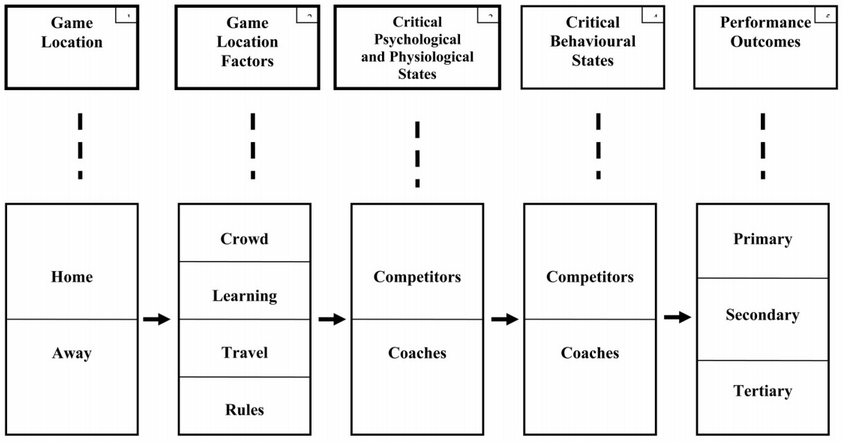
\includegraphics[width=\textwidth]{carron-loughead-bray-framework.png}
    \caption{Framework for game location research. Taken from \citet{bib:carron-loughead-bray-2005}.}
    \label{fig:carron-loughead-bray-framework}
\end{figure}

The framework has been proven useful for providing guidelines on what factors to examine when researching the home ground advantage.

To quantify the home ground advantage, \citet{bib:goddard-2006} collected match results for 35 consecutive seasons in English league football. He looked at the different outcomes of the matches, and how victories are affected by playing at home versus playing away. He also recorded the number of goals scored by the teams over the same period. A summary of his findings is shown in \refertable{tab:goddard-home-results}. The findings clearly show that, even though it has declined the later years, there is still a significant difference between the average performance of the home team and the away team. \citet{bib:bialkowski-lucey-carr-yue-sridharan-matthews-2014} studied teams' style of play. They found that the home team tend to play more in the attacking third of the pitch, which may help explain the difference in number of goals scored between the home and away teams.

There are several other factors influencing the home ground advantage. \citet{bib:pollard-2008} also did a state-of-the-art review on the home ground advantage. He mention how increased travelling distance might increase the home ground advantage, but that the research has shown inconclusive results. The advantage is, however, reduced in local derbies, such as when Arsenal play against Tottenham, two teams with home grounds only $6.6$ km. apart. \citet{bib:pollard-2008} also mention a referee bias. There is evidence that the referee decisions favor the home team. One example is the number of bookings, where the home team is given less bookings that the away team. The bias has been demonstrated in a laboratory setting, where the committed fouls are considered and compared \citep{bib:pollard-2008}. The findings are supported by \citet{bib:nevill-ballmer-williams-2002}, who analyzed 40 referees assessments of an English Premier League match between Liverpool and Leicester City. The referees were exposed to either an audible crowd noise group or no sound at all. The officials in the audible noise group called significantly fewer fouls against the home team than the referees in the silent group. Lastly, \citet{bib:pollard-2008} present research supporting the factors presented in the framework of \citet{bib:carron-loughead-bray-2005}, as well as the special tactics discovered by \citet{bib:bialkowski-lucey-carr-yue-sridharan-matthews-2014}

\begin{table}
    \centering
    \begin{tabulary}{\textwidth}{| L | L | L | L | L |}
        \hline
                                        & \multicolumn{4}{c |}{\textbf{Period}}                                                         \\\hline
        \textbf{Match results (\%)}     & \textbf{1970–1980}    & \textbf{1980–1990}    & \textbf{1990–2000}    & \textbf{2000–2005}    \\\hline\hline
        Home win                        & $50.3$                & $48.8$                & $46.4$                & $45.4$                \\\hline
        Draw                            & $28.6$                & $26.7$                & $27.6$                & $27.5$                \\\hline
        Away win                        & $21.0$                & $24.5$                & $25.9$                & $27.2$                \\\hline\hline
        \textbf{Goals per match (avg.)} &                       &                       &                       &                       \\\hline
        Home team                       & $1.58$                & $1.60$                & $1.51$                & $1.50$                \\\hline
        Away team                       & $0.97$                & $1.06$                & $1.08$                & $1.10$                \\\hline
    \end{tabulary}
    \caption {Trends in home ground advantage in the period 1970-2005. Taken from \citet{bib:goddard-2006}.}
    \label{tab:goddard-home-results} 
\end{table}

\subsection{Attacking and defensive strengths}

Several studies mention the importance of modelling a team's playing abilities, usually in the form of attacking and defensive strengths. However, the way team strengths are modelled have changed over the years.

In the early studies, like that of \citet{bib:maher-1982}, only the number of goals scored and conceded were used for calculating the team strengths. Usually, a team's attacking strength represents their ability to score goals, when their defensive strength represents their ability to avoid conceding goals. \citet{bib:maher-1982} modelled four different strengths for each team; attacking strength when playing at home, defensive strength when playing at home, attacking strength when playing away, and defensive strength when playing away. The distinction between home and away strengths is found in almost every reviewed model, either in the form of separate strengths, or by adding some sort of home ground advantage parameter to the model itself. While the strengths in the model of \citet{bib:maher-1982} do not change over the course of a season, later goal-based studies, like \citet{bib:dixon-coles-1997} and \citet{bib:rue-salvesen-2000}, agree that the strengths of a team vary over time, and that the recent results are more important than older results when modelling the current strengths. Some later models, like that of \citet{bib:cattelan-varin-firth-2013}, focus match outcomes, rather than the number of goals scored. They model a team's strengths at time-step $i$ by the strength at time-step $i-1$ and the number of points achieved in the most recent match.

When adjusting the teams' strengths, the models above do not differentiate "expected" results from those that do not fit the models. For example how lower ranked teams are "expected" to lose against higher ranked teams. The results of a match where the \ordinalnum{1} ranked team loses $0-2$ at home against the \ordinalnum{17} ranked team are treated equally to the results where the \ordinalnum{17} ranked team loses $0-2$ at home against the \ordinalnum{1} ranked team. The probabilities of the two outcomes are quite different, but this difference is not used when adjusting the strengths of the two teams. In the model of \citet{bib:hvattum-arntzen-2010}, the current rank of the two competing teams are taken into account. The difference in rank forms the basis for the ELO rating system.

The system of \citet{bib:constantinou-fenton-neil-2012} takes it a step further. In their system, \citet{bib:constantinou-fenton-neil-2012} do not care about what teams are playing. They consider the teams' current strengths only. To model a team's current strength, \citet{bib:constantinou-fenton-neil-2012} make use of the total number of points accumulated the last three seasons and the number of points accumulated so far the current season, supplemented by the expected number of points for the remaining matches. Team strength is further adjusted using subjective information not captured by previous results (see \refersection{subsec:pi-football}). Another quite unique feature in the model of \citet{bib:constantinou-fenton-neil-2012} is the use of a team's current form. Other models also make use of the recent results of a team, but the model of \citet{bib:constantinou-fenton-neil-2012} measure the recent results of a team according to the expected results, indicating whether a team currently has a good run. In addition, the form is adjusted using the availability of important players.

\subsection{Team characteristics}

Several models try to incorporate the characteristics of football teams in some way. This is usually incorporated in the form of attacking and defensive strengths, number of goals scored per match etc. One shortcoming in these models is the failure to capture how the teams actually play. How do the teams build their attacks? What tactical decisions are made by the teams? These, and similar question, are important to ask, as they are definitive of how the teams play, and thus how the match is played (\citet{bib:pollard-reep-1997}, \citet{bib:bialkowski-lucey-carr-yue-sridharan-matthews-2014}, \citet{bib:hirotsu-wright-2003}).

\subsubsection{Style of play}

\citet{bib:pollard-reep-1997} created a model to capture a team's characteristics. They used a so-called "team possession" as the basic unit of their model. A team possession starts when a player gains possession of the ball, except for when the ball is received from a team member. The receiving player must have good enough control over the ball to be able to deliberately influence the direction of the ball. A team possession ends when one of the following events occur: (a) the ball goes out of play; (b) the ball touches a player of the opposing team (a momentary touch not significantly altering the ball direction is excluded); and (c) an infringement of the rules takes place.

A team possession consists of several components, like passes, throw-ins etc. To assess the effectiveness of the components, the outcome of a team possession need to be quantified. Several outcomes were considered, such as whether the possession ended in a goal, a shot etc. The authors finally composed a outcome measure called "yield". Each outcome is classified by two variables: type of possession and zone of origin. The type of a possession is either free play or set play (like free kicks). The pitch is divided into six different zones, slicing the pitch in equal parts \citep{bib:pollard-reep-1997}.
\begin{equation}
    p_{ij} = \sum_{k=1}^{n_{ij}} \frac{p_{ijk}}{n_{ij}}
    \label{eq:team-possession-probability}
\end{equation}

$p_{ij}$ denotes the probability of scoring after a team possession of type $j$ (1 for open play, 2 for set play) originating in zone $i = 1, ..., 6$. The probability is calculated using \referequation{eq:team-possession-probability}, where $p_{ijk}$ is the $k^{th}$ team possession of type j originating in zone i and $n_{ij}$ is the total number of team possessions of type j originating in zone i. Each recorded team possession is assigned a value $p_{ij}$, defined by the outcome of the possession and the zone of origin of the next team possession. For example, if a team possession ends with the other team regaining the ball in zone 3, then the first team possession will be assigned a value of $-p_{31}$, indicating that the initial team possession ended in favor of the opposing team \citep{bib:pollard-reep-1997}. Using the values $p_{ij}$, the average outcome value for team possessions can be calculated. The average outcome value of a team possession of type j originating in zone i is called the yield $y_{ij}$. The process of setting the values for all $y_{ij}$ is done iteratively.

The yield value can be used to quantify the actual outcome of a team possession. It can also be used to assess the effectiveness of a particular game strategy, by for example taking the mean yield of all team possessions in which the strategy was used. Different strategies can then be compared. \citet{bib:pollard-reep-1997} supplies an example of such a comparison, based on statistics from the World Cup of 1986 in Mexico. The example situation is a throw-in in zone 6. Per 1000 team possessions recorded in the cup, throwing the ball towards the goalmouth had a yield of $21.7$, compared to $3.50$ for a short throw to a nearby team member \citep{bib:pollard-reep-1997}.

\citet{bib:pollard-reep-1997} conclude in their article that fans, media, coaches and players are all sceptical about the suggestion that a statistician might have something useful to provide for a team's tactical analysis, and that a coach's subjective opinions on how to run the game triumphs any number the statistician provide. They suggest using the recorded yields as guidelines on what to base a team's strategy upon. They show examples of actions that provide different yields, such as a zone five free kick; direct shot vs pass to team member, and open field play; running with the ball vs long passes forward vs short passes.

\subsubsection{Team formation}

\citet{bib:bialkowski-lucey-carr-yue-sridharan-matthews-2014} take a closer look on what defines a team's formation, and how it can be identified. Their research question is as following; "Given all the player and ball tracking data of a team in a season, what team-based features can adequately discriminate a team’s behavior?". They answer this question using an in-depth model of a football match, focusing on team formations.

During a match, each player is assigned a role. A given role can only be assigned to one player at any given time, but players may change roles during the match. A role is described by its position relative to the other roles (the left back plays to the left of the central defenders, etc.). A formation assigns a space on the pitch to each player at every time-frame (capturing 10 frames per second). Identifying a team's formation based on player tracking data can be framed as a minimum entropy data partitioning problem \citep{bib:bialkowski-lucey-carr-yue-sridharan-matthews-2014} for each time-frame. An example of such a problem is shown in \referfigure{fig:lee-choi-clustering}. This problem can be modelled as a linear assignment problem, which the authors solve by using the Hungarian algorithm \citep{bib:kuhn-1955}.

\begin{figure}
    \centering
    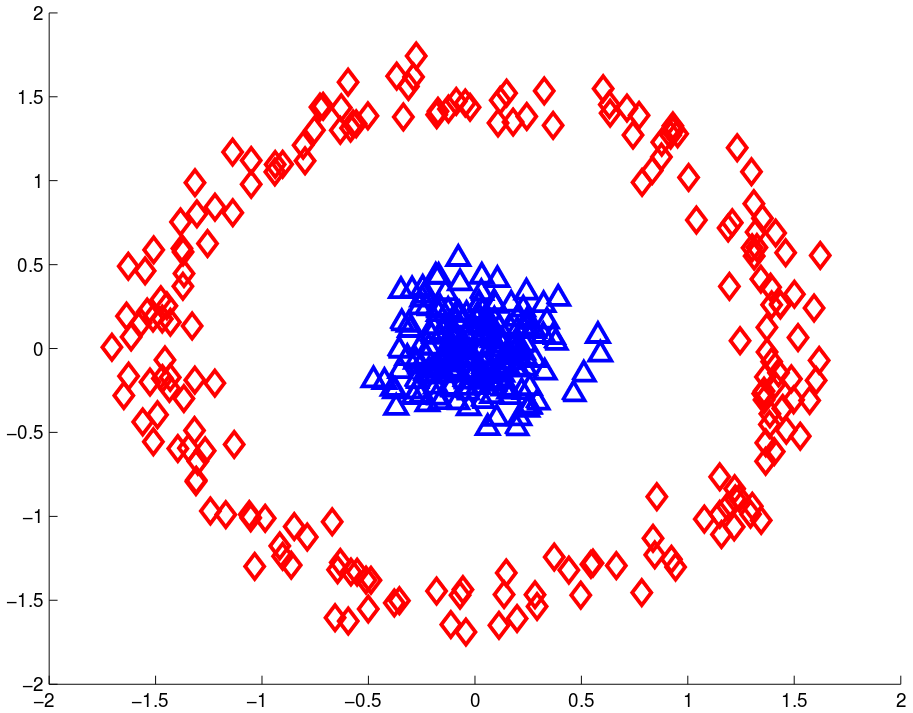
\includegraphics[width=0.75\textwidth]{lee-choi-clustering.png}
    \caption{An example of clustering a ring. Taken from \citet{bib:lee-choi-2004}.}
    \label{fig:lee-choi-clustering}
\end{figure}

Using only player tracking data and ball events for a given team, \citet{bib:bialkowski-lucey-carr-yue-sridharan-matthews-2014} created a model for identifying different teams. The model is based on three different match descriptors;

\begin{itemize}
    \item \textbf{Match statistics:} Various statistics registered during a match. The statistics capture team and individual behavior, and include variables like corners, catches, goals, bookings, chances, shots, etc. Each match statistics event is associated with a timestamp and a location on the pitch.
    \item \textbf{Ball occupancy:} The pitch is divided into a $10x8$ cell big spatial grid. The ball occupancy is calculated for each cell in the grid, and gives a quantitative description of how often the team was in possession of the ball at each cell during a match. This descriptor captures where the different teams like to put pressure during a match. An example of a ball occupancy map is given in \referfigure{fig:bialkowski-et-al-ball-occupancy}. The map shows how the team tend to attack on the left side of the pitch \citep{bib:bialkowski-lucey-carr-yue-sridharan-matthews-2014}.
    \item \textbf{Formation descriptor:} The formation of a team is described as above. The formation description is defined as a $MxN$ matrix, where $M$ is the number of cells in the field and $N$ the number of roles (set to 10, excluding keeper). The descriptor describes where the players of different roles tend to move on the pitch. Ten examples of team formation descriptor depictions are shown in \referfigure{fig:bialkowski-et-al-formation-descriptors}.
\end{itemize}

\begin{figure}
    \centering
    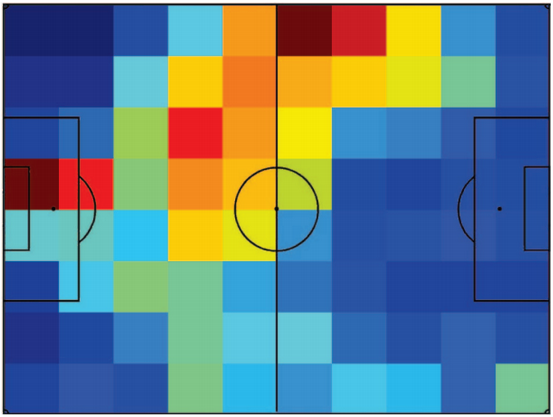
\includegraphics[width=0.75\textwidth]{bialkowski-et-al-ball-occupancy.png}
    \caption{An example ball occupancy map (over a match half) for a team attacking from left to right. Taken from \citet{bib:bialkowski-lucey-carr-yue-sridharan-matthews-2014}.}
    \label{fig:bialkowski-et-al-ball-occupancy}
\end{figure}

\begin{figure}
    \centering
    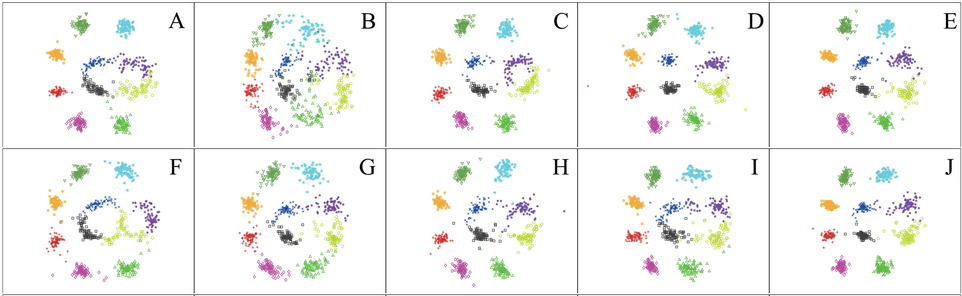
\includegraphics[width=\textwidth]{bialkowski-et-al-formation-descriptors.png}
    \caption{Depictions of team formation descriptors for a team attacking from left to right. The colors represent the different roles. Only the centroid for each role for each match is depicted. Taken from \citet{bib:bialkowski-lucey-carr-yue-sridharan-matthews-2014}.}
    \label{fig:bialkowski-et-al-formation-descriptors}
\end{figure}

\citet{bib:bialkowski-lucey-carr-yue-sridharan-matthews-2014} set up an experiment to test the accuracy of their model. The experiment was conducted using "leave-one-out" cross-validation, training their model on all but one match for each team. Using data from a top-tier professional soccer league, the model correctly predicted the team in over 70\% of the cases. These results clearly show that "teams have a true underlying signal which can be encapsulated in the way the team moves in formation over time" \citep{bib:bialkowski-lucey-carr-yue-sridharan-matthews-2014}. In addition, there is also additional information to gain from where different teams put pressure during matches, and how much they interact with the ball throughout a match. This information, combined with the attacking and defensive strengths of a team, might be useful in prediction of match outcomes \citep{bib:bialkowski-lucey-carr-yue-matthews-2014}. For example, knowing that a team plays a lot on their wings, crossing the ball into the goalmouth, whilst the opposing team has good, strong central defenders might tell something about how the match will progress.

The experiments of \citet{bib:bialkowski-lucey-carr-yue-sridharan-matthews-2014} also showed that teams are rather rigid in the way the play across a season, which they suggest could be used as a powerful prior for preparing for upcoming matches.

Team style is a very subjective and high-level attribute, especially in football, and is therefore hard to segment into discrete parts. Team style covers all aspect of play \citep{bib:bialkowski-lucey-carr-yue-sridharan-matthews-2014}. The way they quantified team style was by computing a linear combination of prior behavior styles. Given a set of team behavior descriptors, they discovered a discrete set of play styles using k-means clustering. Using different values for $k$, completely different patterns were discovered. Every team's style was classified uniquely, with each style modelled as a weighted combination of different styles. This makes sense, as a team might play a pressing game one match, and defending the next \citep{bib:bialkowski-lucey-carr-yue-sridharan-matthews-2014}. \referfigure{fig:bialkowski-et-al-team-style-clusters} shows an example of how different values for $k$ affect the style clustering descriptors. According to \citet{bib:bialkowski-lucey-carr-yue-sridharan-matthews-2014}, these descriptors can be used for predicting the results of future matches.

\begin{figure}
    \centering
    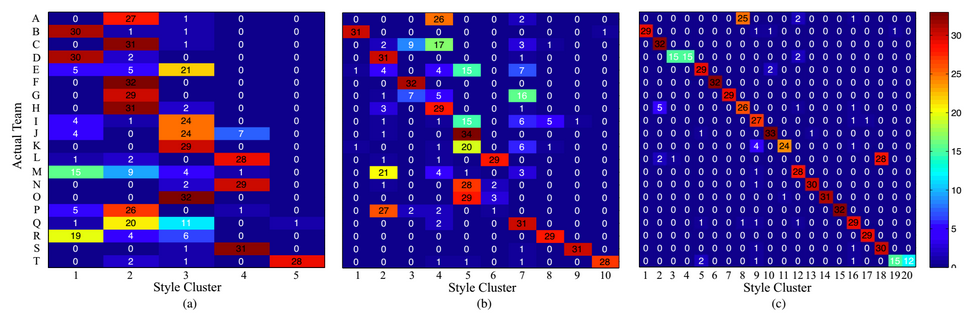
\includegraphics[width=\textwidth]{bialkowski-et-al-team-style-clusters.png}
    \caption{Clustering descriptor of each match half for different values for $k$. (a) 5, (b) 10, (b) 20. Taken from \citet{bib:bialkowski-lucey-carr-yue-sridharan-matthews-2014}.}
    \label{fig:bialkowski-et-al-team-style-clusters}
\end{figure}

In addition to identifying teams based on match data, \citet{bib:bialkowski-lucey-carr-yue-sridharan-matthews-2014} also used the system for predicting team behavior and how matches are played. Given the identities of two opposing teams, they were able to precisely predict the locations of the players in the different roles in most matches. To do this, they used k-NN regression using the learnt team style priors as input. Their predictions estimated with an average of 2 meters error per role for most matches.

In the future, \citet{bib:bialkowski-lucey-carr-yue-sridharan-matthews-2014} plan to use their system for both short-term (who will pass to to etc.) and long-term (match outcome) predictions.


\subsection{Team psychology}

In some cases, the psychology of the competing teams can have an impact on the final results.

\citet{bib:goddard-asimakopoulos-2004} mention the importance of "significant" matches. A match is significant for a team if it is possible (before the match is played) for the team to either win the championship, or to be promoted or relegated, assuming all other teams in contention for the same outcome score one point each on average. According to \citet{bib:goddard-asimakopoulos-2004}, teams are more likely to over-perform in significant matches. As a result, if a match is significant for one team, but not for the other, the incentive difference is likely to influence the final result.

Early elimination from knockout tournaments may also influence a team's results in subsequent league matches. On the one side, a team recently eliminated from a tournament may able to concentrate more on the league, consequently improving their league results. On the other side, elimination might reduce the overall team spirit and confidence of a team, deteriorating the league results. Statistics suggest the latter effect dominates the former \citep{bib:goddard-asimakopoulos-2004}.

\citet{bib:rue-salvesen-2000} mention the effect of superiority. If team A is superior to team B, in terms of team strength and historical results, A tend to underestimate B, changing the outcome probabilities in favor of B. The effect is reversed if A is far too superior, so that B develop an inferiority complex facing A \citep{bib:rue-salvesen-2000}.
\section{Measuring the accuracy of a prediction model}
\label{sec:background-rps}

Measuring the accuracy of a prediction model is a crucial part of its validation \citep{bib:constantinou-fenton-neil-2012}. There are several ways of evaluating the accuracy of a prediction model, with different degrees of quality.

\citet{bib:constantinou-fenton-2012} present five scoring rules, and show why they are not able to correctly evaluate the accuracy of two hypothetical prediction models. They then present the \gls{rps}, an alternative scoring rule. The study presents two prediction models, $\alpha$ and $\beta$, and their predicted probabilities for the outcomes of five hypothetical matches, numbered $1-5$. \cref{tab:rps-matches} shows the five matches together with the predicted probability distributions for the two models. As can be seen from the figure, model $\alpha$ produces the best prediction for all five matches.
\begin{table}
    \centering
    \begin{tabulary}{\textwidth}{| C | C | C | C | C | C | C |}
        \hline
        \textbf{Match}  & \textbf{Model}    & \textbf{p(H)} & \textbf{p(D)} & \textbf{p(A)} & \textbf{Result}   & \textbf{'Best model'} \\\hline
        1               & $\alpha$          & 1             & 0             & 0             & H                 & $\alpha$ \\\hline
                        & $\beta$           & 0.9           & 0.1           & 0             &                   &  \\\hline
        2               & $\alpha$          & 0.8           & 0.1           & 0.1           & H                 & $\alpha$ \\\hline
                        & $\beta$           & 0.5           & 0.25          & 0.25          &                   &  \\\hline
        3               & $\alpha$          & 0.35          & 0.3           & 0.35          & D                 & $\alpha$ \\\hline
                        & $\beta$           & 0.6           & 0.3           & 0.1           &                   &  \\\hline
        4               & $\alpha$          & 0.6           & 0.3           & 0.1           & H                 & $\alpha$ \\\hline
                        & $\beta$           & 0.6           & 0.1           & 0.3           &                   &  \\\hline
        5               & $\alpha$          & 0.5           & 0.45          & 0.05          & H                 & $\alpha$ \\\hline
                        & $\beta$           & 0.55          & 0.10          & 0.35          &                   &  \\\hline
    \end{tabulary}
    \caption{Predicted probabilities by the two hypothetical prediction models, $\alpha$ and $\beta$, for five hypothetical matches. Taken from \citet{bib:constantinou-fenton-2012}.}
    \label{tab:rps-matches} 
\end{table}

\citeauthor{bib:constantinou-fenton-2012} give the following reasons as to why model $\alpha$ is the best model:
\begin{itemize}
    \item \textbf{Match 1:} Model $\alpha$ predicts the correct outcome with total certainty, and must therefore score higher than model $\beta$.
    \item \textbf{Match 2:} Both models assign the highest probability to the correct outcome, with the two other outcomes evenly distributed. Since model $\alpha$ assigns the correct outcome a higher probability than model $\beta$, model $\alpha$ must score higher.
    \item \textbf{Match 3:} Both models assign the same probability to the correct outcome. Still, model $\alpha$ is more accurate, as its overall distribution of probabilities is more indicative of a draw than that of model $\beta$.
    \item \textbf{Match 4:} Both models assign the same probability to the correct outcome. Still, model $\alpha$ is more accurate, as its overall distribution of probabilities is more indicative of a home win than that of model $\beta$.
    \item \textbf{Match 5:} Even though model $\alpha$ predicts the correct outcome with a lower probability than $\beta$, the distribution of model $\alpha$ is more indicative of a home win than that of model $\beta$. According to \citeauthor{bib:constantinou-fenton-2012}, this is easily explained by considering a gambler who is confident that the home team will not lose, and seeks to place a \textit{lay} bet (a bet that is successful if the home team wins, or the match ends with a draw). If $\alpha$ and $\beta$ are forecasts by two different bookmakers, bookmaker $\alpha$ will pay less for the winning bet.
\end{itemize}

\cref{tab:rps-comparison} shows how five different scoring rules score models $\alpha$ and $\beta$. A check mark indicates that the scoring rule correctly considers model $\alpha$ more accurate than model $\beta$. A single cross indicates that the scoring rule incorrectly considers the models equally accurate. Two crosses indicate that the scoring rule incorrectly considers model $\beta$ more accurate than model $\alpha$.
\begin{table}
    \centering
    \begin{tabulary}{\textwidth}{| C | C | C | C | C | C |}
        \hline
        \textbf{Match (model)} & \textbf{Binary Decision Score}     & \textbf{Brier Score}  & \textbf{Geometric Mean Score} & \textbf{Information Loss Score}   & \textbf{MLLE Score}   \\\hline
        1                       & \cmark                            & \cmark                & \cmark                        & \cmark                            & \cmark                \\
        ($\alpha$)              & 1                                 & 0                     & 1                             & 0                                 & 0                     \\
        ($\beta$)               & 0                                 & 0.02                  & 0.9                           & 0.152                             & -0.1054               \\\hline
        2                       & \xmark                            & \cmark                & \cmark                        & \cmark                            & \cmark                \\
        ($\alpha$)              & 1                                 & 0.06                  & 0.8                           & 0.3219                            & -0.2231               \\
        ($\beta$)               & 1                                 & 0.375                 & 0.5                           & 1                                 & -0.6931               \\\hline
        3                       & \xmark                            & \cmark                & \xmark                        & \xmark                            & \xmark                \\
        ($\alpha$)              & 0                                 & 0.735                 & 0.3                           & 1.7369                            & -1.2039               \\
        ($\beta$)               & 0                                 & 0.86                  & 0.3                           & 1.7369                            & -1.2039               \\\hline
        4                       & \xmark                            & \xmark                & \xmark                        & \xmark                            & \xmark                \\
        ($\alpha$)              & 1                                 & 0.26                  & 0.6                           & 0.7369                            & -0.5108               \\
        ($\beta$)               & 1                                 & 0.26                  & 0.6                           & 0.7369                            & -0.5108               \\\hline
        5                       & \xmark                            & \xmark\xmark          & \xmark\xmark                  & \xmark\xmark                      & \xmark\xmark          \\
        ($\alpha$)              & 1                                 & 0.455                 & 0.5                           & 1                                 & -0.6931               \\
        ($\beta$)               & 1                                 & 0.335                 & 0.55                          & 0.8625                            & -0.5978               \\\hline
    \end{tabulary}
    \caption{Comparison of different scoring rules. Taken from \citet{bib:constantinou-fenton-2012}.}
    \label{tab:rps-comparison} 
\end{table}

\cref{eq:rps-equation-original} presents the \gls{rps}, introduced by \citet{bib:epstein1969scoring}.
\begin{equation}
    RPS = \frac{1}{r-1} \sum_{i=0}^{r-1} \bigg( \sum_{j=0}^{i} (p_{j} - e_{j}) \bigg) ^ {2},
    \label{eq:rps-equation-original}
\end{equation}
where $r$ is the number of outcomes ($r = 3$ for football matches), $p_{j}$ the predicted probability for outcome $j$, and $e_{j}$ the observed value for outcome $j$ (1 if $j$ is the observed outcome, 0 otherwise). 

The \gls{rps} calculates the difference between the cumulative distributions of the predicted and observed probabilities. Lower scores indicate better predictions. \cref{tab:rps-rps-scores} shows the calculated \gls{rps} values for the predictions of model $\alpha$ and model $\beta$. As can be seen from the table, \gls{rps} correctly considers model $\alpha$ more accurate than model $\beta$ for all matches.
\begin{table}
    \centering
    \begin{tabulary}{\textwidth}{| C | C | C | C | C |}
        \hline
        \textbf{Match}  & \textbf{Model}    & $\sum_{j=0}^{i=0,1,2} p_{j}$  & $\sum_{j=0}^{i=0,1,2} e_{j}$  & \textbf{\gls{rps}}   \\\hline
        1               & $\alpha$          & 1, 1, 1                       & 1, 1, 1                       & (0.0000) \\
                        & $\beta$           & 0.90, 1, 1                    & 1, 1, 1                       & 0.0050 \\\hline
        2               & $\alpha$          & 0.80, 0.90, 1                 & 1, 1, 1                       & (0.0250) \\
                        & $\beta$           & 0.50, 0.75, 1                 & 1, 1, 1                       & 0.1562 \\\hline
        3               & $\alpha$          & 0.35, 0.65, 1                 & 0, 1, 1                       & (0.1225) \\
                        & $\beta$           & 0.60, 0.90, 1                 & 0, 1, 1                       & 0.1850 \\\hline
        4               & $\alpha$          & 0.60, 0.90, 1                 & 1, 1, 1                       & (0.0850) \\
                        & $\beta$           & 0.60, 0.70, 1                 & 1, 1, 1                       & 0.1250 \\\hline
        5               & $\alpha$          & 0.50, 0.95, 1                 & 1, 1, 1                       & (0.1262) \\
                        & $\beta$           & 0.55, 0.65, 1                 & 1, 1, 1                       & 0.1625 \\\hline
    \end{tabulary}
    \caption{RPS values for the predictions of model $\alpha$ and model $\beta$. Taken from \citet{bib:constantinou-fenton-2012}.}
    \label{tab:rps-rps-scores} 
\end{table}

When using \gls{rps} to evaluate a prediction model over several matches, \citet{bib:constantinou-fenton-2012} suggest using either the arithmetic mean over the individual scores, or the total of the individual scores.
\section{Applying predictions to betting}
\label{sec:background-betting}

When applying prediction models in a betting setting, the goal of a model changes from predicting the correct result to make a profit from the predictions.

\subsection{Background}

In order to understand how to beat the bookmakers, one must first understand how their odds are formed. The expected margin (gain) of a bookmaker on a football match is represented as.
\begin{equation}
    E(M) = 1 - \sum_{i=0}^{2} P_{i} * w_{i} * d_{i},
    \label{eq:vlastakis-dotsis-markellos-margin}
\end{equation}
where $i$ correspond to the different outcomes ($0$ for home victory, $1$ for draw, $2$ for away victory). The expected margin $M$ of a match depends both on the probability $P_{i}$ of each outcome, the percentage $w_{i}$ of bets placed on each outcome, and the given odds $d_{i}$ for each outcome \citep{bib:vlastakis-dotsis-markellos-2009}.

Bookmakers are interested in keeping a stable profit, and set their prices accordingly \citep{bib:vlastakis-dotsis-markellos-2009}. \cref{eq:vlastakis-dotsis-markellos-margin} implies there are different ways for bookmakers to set their prices. One example is to accurately forecast the game outcomes so that the odds reflects the expectations. Another way is to forecast the distribution of bets placed on each outcome. Finally, it is possible to combine the two \citep{bib:vlastakis-dotsis-markellos-2009}.

As the true outcome probabilities are not known, the bookmakers can only control the values of $d_{i}$. The values of $w_{i}$ change (usually according to the corresponding $d_{i}$), and are controlled by the bettors. Therefore, to ensure a profit, the bookmakers must ensure that
\begin{equation*}
    \forall i \in \{0, 1, 2\}: w_{i} * d_{i} < 1
    \quad \text{or, more generally,} \quad
    \sum_{i=0}^{2} (1 - w_{i} * d_{i}) > 0.
\end{equation*}

To calculate the actual margins for a single match, one need to know both the odds on every outcome and how the bets are distributed. The odds are publicly available, but the bet distributions are not. One can therefore not calculate the actual margin, but rather an \textit{implied} margin. According to \citet{bib:vlastakis-dotsis-markellos-2009}, the standard way of doing this is by assuming the bets are evenly distributed across all outcomes. That is,  
\begin{equation*}
    \forall i \in \{0, 1, 2\}: w_{i} = \frac{1}{3}.
\end{equation*}
It is further assumed that the odds are set according to the true probabilities of each outcome. The true probabilities are usually estimated by the bookmaker's own odds compilers \citep{bib:vlastakis-dotsis-markellos-2009}. Assuming the odds are set according to the true probabilities, the fair odds for outcome $i$ is then $\frac{1}{P_{i}}$. However, if the odds are based on the true probabilities, then the expected bookmaker margin would be zero (this can be seen by replacing $d_{i}$ with $P_{i}^{-1}$ in \cref{eq:vlastakis-dotsis-markellos-margin}). Therefore, the actual odds correspond to \textit{implied} probabilities ($P_{i}'$) somewhat larger than the true probabilities. The expected margin of a bookmaker can then be seen as
\begin{equation}
    E(M') = \Bigg(\sum_{i=0}^{2} P_{i}'\Bigg) - 1 = \Bigg(\sum_{i=0}^{2} \frac{1}{d_{i}}\Bigg) - 1.
    \label{eq:bookmaker-implied-margin}
\end{equation}

When Liverpool played at home against West Ham on December 11, 2016, the average odds were $1.29$, $6.22$, and $10.23$ for home, draw, and away, respectively \citep{bib:odds-portal}. By \cref{eq:bookmaker-implied-margin}, the expected margins of the combined betting marked was $\frac{1}{1.29} + \frac{1}{6.22} + \frac{1}{10.23} - 1 = 0.034$. The bookmakers were expected to gain a profit of $3.4\%$. For a prediction model to make a profit against the bookmakers, it must therefore not just beat the predictions of the bookmakers. It must also beat the built-in margins.

\subsection{Money management strategies}
\label{sec:betting-strategies}

When deciding whether to place a bet, one must compare the probabilities of the outcomes calculated by the prediction model with the odds offered by the bookmakers. The expected gain for a given bet can be calculated as $P_{i} * d_{i} - 1$, and bets are usually placed on outcomes where the gain is expected to be positive. It is normal to set a threshold, $\tau$ on the minimum discrepancy level allowed. This is done to take the built-in profit margins of the bookmakers into account, increasing the level of confidence needed in order to place a bet.

When an expected profitable match is found, one must be able to decide how much money to place on the bet. Consider the following scenarios:
\begin{itemize}
    \item \textbf{Match 1}: $P_{2} = 0.20, d_{2} = 6.0$.
    \item \textbf{Match 2}: $P_{0} = 0.60, d_{0} = 2.0$.
\end{itemize}
The expected gain for each of the bets is $P_{i} * d_{i} - 1 = 0.2$. However, the amount of money to put on each of the bets is not clear. While the odds of Match 2 is clearly lower than that of Match 1, one has to wager more money on Match 2 in order to win the same amount of money. \citet{bib:langseth-2013} presents five different strategies deciding on how much money to place on each bet, based on the outcome probability $P_{i}$ and odds $d_{i}$, and the bankroll $C$ of the bettor. Each strategy output the amount $c_{i}$ to place on a given bet, where $1$ is the unit size. The strategies are as follows:
\begin{itemize}
    \item \textbf{Fixed bet:} The simplest strategy. For each feasible bet, place the same amount of money. $c_{i} \propto 1$.
    
    \item \textbf{Fixed return:} Each bet is assured to produce the same profit. $c_{i} \propto \frac{1}{d_{i}}$. This results in lower amounts placed on high-odds bets.
    
    \item \textbf{Kelly ratio:} \citet{bib:kelly-1956} proposed a strategy based on a decision-theoretic approach. In his setup, the utility of having a bankroll of $C$ after a bet is set to $\ln(C)$. The utility for going broke therefore approaches $- \infty$. The expected utility of a bet $c_{i}$ is $P_{i} * \ln(C + d_{i} c_{i}) + (1 - P_{i}) * \ln(C - c_{i})$. The utility is then maximized by choosing $c_{i} = C * \frac{P_{i} d_{i} - 1}{d_{i} - 1}$. To reduce the potential of emptying the bankroll in the early stages, \citet{bib:langseth-2013} proposed a modification of the strategy, where the size of $c_{i}$ is limited not to exceed a predefined value, $C_{0}$, chosen to be "much smaller than the bankroll".
    
    \item \textbf{Markowitz portfolio management:} In the Markowitz portfolio management strategy, one look at a collection of bets over a game-week. The goal is to find an allocation of bets that maximizes $\sum_{i=1}^{n} (\mathbb{E}[\Delta_{i}] - \nu Var[\Delta_{i}])$ under the constraint that the bets during the game-week sum to a predefined value $C_{0}$. $\nu$ represents the accepted level of risk. The dual representation of the optimization problem is then to minimize $\sum_{i=1}^{n} Var[\Delta_{i}]$ under the constraints $\sum_{i=1}^{n} c_{i} = C_{0}$ and $\sum_{i=1}^{n} \mathbb{E}[\Delta_{i}] = \mu$. $\mu$ is then the representation of the accepted risk level.
    
    \citet{bib:langseth-2013} used three different values for $\mu$ in his experiments:
    \begin{itemize}
        \item \textbf{Risk-averse:} $\mu = \mu_{\downarrow} = (\sum_{i=1}^{n} P_{i} d_{i}) / n - 1$
        \item \textbf{Risk-seeking:} $\mu = \mu^{\uparrow} = \max_{i} P_{i} d_{i} - 1$
        \item \textbf{Intermediate:} $\mu = (\mu_{\downarrow} + \mu^{\uparrow}) / 2$
    \end{itemize}
    
    \item \textbf{Variance-adjusted:} \citet{bib:rue-salvesen-2000} proposed a strategy for minimizing the difference between the expected profit and the variance of the profit. According to \citet{bib:langseth-2013}, the variance-adjusted strategy can be seen as a simplification of the Markowitz portfolio management strategy. After placing a bet, the difference is $P_{i} d_{i} c_{i} - P_{i}(1 - P_{i})(d_{i} c_{i})^{2}$, which is minimized by choosing $c_{i} = (2 d_{i} (1 - P_{i}))^{-1}$.
\end{itemize}
In his paper, \citet{bib:langseth-2013} compared the profitability of three prediction models using the presented strategies. The experiments were conducted over the course of two consecutive seasons of the English Premier League. In the first season, each of the different prediction models were able to make a profit. However, the three prediction models had their own respective most profitable betting strategy. For the second season, only a single combination of prediction model and betting strategy was able to make a profit. The profit, however, was of only $0.4\%$. These results highlight the importance of choosing a betting strategy that suits the prediction model. It should be noted that the threshold $\tau$ was $0$ during these experiments, and that loosing less than the built-in bookmaker margin therefore can be considered "decent" \citep{bib:langseth-2013}.

In addition to the strategies presented by \citet{bib:langseth-2013}, \citet{bib:rue-salvesen-2000} presented another strategy, based on the mean and variance of a bet's profit. From outcome $i$ of a match, let $c_{i}$ be the corresponding bet. The mean and variance of a bet's profit is found using outcome probability $P_{i}$ and outcome odds $d_{i}$. The optimal bet for a match is then found as
\begin{equation*}
    \underset{c_{i} > 0}{\arg\max}\ U(\{c_{i}\}), \quad \text{where} \quad U(\{c_{i}\}) = \text{E(profit)} - \text{Var(profit)} = c_{i} (\mu_{i} - c_{i} \sigma_{i}^{2})
\end{equation*}
The solution is $c_{i} = \max \{ 0, \mu_{i}/(2 \sigma_{i}^{2}) \}$. In order to place only one bet per match, $i$ is chosen to maximize $c_{i} \mu_{i}$.



\subsection{Biases}
\label{subsec:background-betting-biases}

In addition to the bookmakers' built-in margins, there has been observed biases for different kind of bets. These biases are important to consider when placing bets, as they can significantly impact the profitability of a strategy. \citet{bib:constantinou-fenton-2013} present the three most important odds biases:
\begin{itemize}
    \item \textbf{Favorite-longshot bias:} Low-odds bets tend to generate a higher return than high-odds bets. According to \citet{bib:constantinou-fenton-2013}, the strongest hypothesis behind this phenomenon is the bettors' preference in backing risky outcomes. For example, in a match where the probability of a home win is $0.9$, even if the bookmaker sets a fair odds of $1.11$, a typical bettor is reluctant to place $\pounds 100$ bet only to win $\pounds 11$. If the probability of an away win is $0.05$, a typical bettor would be prepared to bet at less than fair odds, for example $15$, because a small bet of $\pounds 10$ can potentially return $\pounds 150$. 
    
    \item \textbf{Home-away bias:} \citet{bib:constantinou-fenton-2013} mention how some researchers consider all home wins and away wins to serve as favorite and longshot outcomes, respectively. On average, away wins can be seen as long shots (as indicated by the home ground advantage), but for a significant portion of matches, this does not hold. \citet{bib:constantinou-fenton-2013} demonstrated the home-away bias by comparing the cumulative returns generated by simulating $\pounds 1$ bets on all home wins, draws, and away wins during seven seasons in four different major leagues.
    
    \item \textbf{Most-likely/least-likely bias:} \citet{bib:constantinou-fenton-2013} also demonstrated how the odds are tailored in favor of the most-likely outcome of a match. By performing a similar simulation to that above, the cumulative loss when betting on all least-likely outcomes was significantly higher than when betting on all most-likely outcomes. These results are in agreement with the favorite-longshot bias, whereby low-odds bets generate higher returns than high-odds ones.
\end{itemize}
\section{\whoscoredplain}

\whoscored\ is a football statistics web site, offering free statistics for almost 500 different leagues and tournaments all over the world (as of \today). Their database is vast, covering matches all the way back to 1999 for some competitions.

\subsection{Match statistics}
\label{subsec:whoscored-match-details}

\whoscored\  offers match statistics on three levels of details: minimum, intermediate, and full.

\subsubsection{Minimum details}

For matches with minimum available details, only the basic information is available: what teams are playing, time elapsed, final result, and kickoff time. The majority of all competitions fall into this category.

\subsubsection{Intermediate details}

For matches with intermediate details, some additional information is included in addition to the basic information: lineups, substitutes, and the most important match events (goals, penalty misses, substitutions, and red and yellow cards).

This was the most detailed level of details from August 2002 throughout the season 2008/2009.

\subsubsection{Full details}

Only a handful of competitions are covered with full match details. In addition to the most basic information, the full details include generic information about the match, such as venue, attendance number, referee, weather conditions, and team managers.

The full details also include a detailed overview of almost every event taking place during the match. Free kicks, tackles, saves, and passes are examples of such events. Each event has several properties, such as location on the pitch, at what time it happened, and players involved. A thorough description of the detailed match data is included in \cref{chp:whoscored-data-description}.

In addition to event data, the full details contain information about the teams' formations: each formation the team used during the match, with player positions, who was captain, and when the formation started and ended.

The full details also include statistics for each participating player. The statistics consist of several metrics, such as the number of tackles, saves, or passes, and how they developed over time. A list of all available metrics is included in \cref{tab:whoscored-player-metrics}.

Lastly, the full details include ratings of all involved players, along with a rating for the team as a whole. The ratings are valued on a scale from 0 through 10, where 10 is the top rating. The ratings are calculated based on the player's contribution to the team.


\subsection{Team and player statistics}

\whoscored\ also offers team and player statistics. Descriptions of the statistics are shown in \cref{tab:whoscored-team-views} and \cref{tab:whoscored-player-views}.
\section{Technologies}

The following technologies have been utilized in this report.


\subsection{Regular expressions}

A regular expression is a string describing a set of strings, a pattern, following given syntax rules. Regular expressions are widely used in text editors, when searching and replacing text based on patterns. Regular expressions are supported by several programming languages, such as JavaScript and Python.

An important part of regular expressions are meta-characters. Meta-characters describe a set of characters, and allow evaluating logical expressions on the string. \cref{tab:regular-expression-meaning} shows some of the most central meta-characters.

\begin{table}
    \centering
    \noindent\begin{tabulary}{\textwidth}{| L | L |}
        \hline
        \textbf{Character}                                              & \textbf{Meaning} \\\hline
        \textasciicircum, \$                                            & Start and end of string \\\hline
        .                                                               & Any character except newline \\\hline
        \textbackslash .                                                & Escaping of a meta-character (in this case \textit{.}) \\\hline
        $[abc]$                                                           & Group of characters (in this case, \textit{a}, \textit{b}, or \textit{c}) \\\hline
        $a|b$                                                             & Logical or of characters (in this case \textit{a} or \textit{b}) \\\hline
        \textbackslash s, \textbackslash d, \textbackslash w            & Whitespace character, digit, and word character \\\hline
        \{m, n\}                                                        & Between \textit{m} and \textit{n} inclusive occurrences of the previous meta-character \\\hline
        ?                                                               & Zero or one occurrences of the previous meta-character \\\hline
        +                                                               & One or more occurrences of the previous meta-character \\\hline
        *                                                               & Zero or more occurrences of the previous meta-character \\\hline
    \end{tabulary}
    \caption{List of central meta-characters used in regular expressions.}
    \label{tab:regular-expression-meaning}
\end{table}


\subsection{HTML}

\gls{html} is the de facto standard markup language for creating web pages. An \gls{html} document is built up by tags describing how the web page should look and behave. Web browsers read \gls{html} documents and present the content accordingly.


\subsection{JavaScript}

JavaScript is a high-level programming language. Together with \gls{html}, JavaScript is a powerful tool supported by just about every modern web browser. JavaScript is versatile, supporting both object oriented-programming and functional programming.

JavaScript is natively supported in \gls{html}, and is extremely useful for creating dynamic web pages. A popular use case for JavaScript is dynamic loading of data without reloading the web page.


\subsection{Python}

Python is a high-level programming language. It supports several programming paradigms, such as imperative, functional, object-oriented, and procedural programming. Python was originally developed as a scripting language, but is today used in several other contexts, such as web servers and desktop applications.

There is a vast community around Python, and countless libraries for everything from web scraping to 3D animation.


\subsection{Tensorflow}

TensorFlow is an open source library for machine learning. TensorFlow performs numerical computations using data flow graphs. The nodes in the graphs represent mathematical operations, while the edges represent the data arrays communicated between the nodes. TensorFlow has a flexible architecture, allowing for parallel computations over several CPUs or GPUs on servers, desktop computers, or mobile devices \citep{bib:tensorflow}.


\subsection{Keras}

Keras is a high-level \gls{ann} API, written in Python. Keras does not implement any form for \gls{ann} functionality itself, but runs on top other libraries, like TensorFlow. Keras was developed with a focus on user friendliness, modularity, and extensibility \citep{bib:keras}.


\subsection{MySQL}

MySQL is a database management system based on \gls{sql}. \gls{sql} is a programming language designed for use with databases. The language is based on relational algebra and calculations, and is mostly used for interacting with relational databases \citep{bib:codd1982relational}.

%========================================================================
%   CHAPTER: THEORY
%========================================================================

\chapter{Theory}
\label{chp:theory}
In this chapter, the general theory used in the rest of the report is presented. This chapter serves as a reference for the later chapters where the theory is applied.
\section{Statistical classification}

Statistical classification is the problem of identifying to what set of categories an observation belongs, given a set of observations with known categories (or classes). A far too well-known classification problem is whether email should be considered "spam" or not. Another well-known example is assigning a diagnosis to a patient, given a description of its symptoms and personal characteristics.

When collecting and analyzing large amounts of data, it is often necessary to separate the different data points into classes. As there are few limitations on how much data a single data point can contain, the classification task can easily become too tough for any human to perform. A digital classifier can then be used instead.

A digital classifier works similarly to the human way. A digital classifier increases its knowledge using a set of known observations and their corresponding classes (the training set). The classifier then applies its obtained knowledge to determine the classes of new observations. This training method is called "supervised learning".

There are several different digital classifier algorithms and systems, such as the \gls{knn} algorithm \citep{bib:peterson-2009}, \glspl{svm} algorithm \citep{bib:noble-2006}, and \glspl{ann} \citep{bib:yegnanarayana-2009}.


\subsection{Overfitting}

For a digital classifier to perform well, it must accurately assign correct classes to different observations. However, it must not blindly learn the mappings for the observations in the training data set. It is important that a classifier generalizes, so that it can accurately map new observations. If a classifier can accurately assign classes to known observations, without accurately classifying new observations the classifier "overfits" on the training data \citep{bib:hawkins2004problem}.

Overfitting usually occurs when a network is too complex. When overfitting, the network memorizes known observations rather than learning the underlying target function. Unknown observations then result in random error or noise.
\section{Artificial neural networks}

An \gls{ann} is a computational model used in computer science, machine learning, and other research areas. \glspl{ann} are loosely modeled after the human brain. The human brain contains vast amounts of nerve cells (neurons), which are highly interconnected, creating a huge network of signal transmission. Each neuron receives an electric signal from all the cells it is connected to (its neighbours). If the signal reaches a certain threshold, the neuron sends a signal on to all its neighbours. The procedure repeats itself, propagating electric signals throughout the brain.

Similarly to the human brain, \glspl{ann} are built up by connecting a set of simple units called \textit{perceptrons}. \footnote{Perceptrons are often referred to as neurons or nodes. In the context of \glspl{ann}, the three are interchangeable.} A perceptron takes in up to several weighted input values. The input values are summarized, usually together with a weighted constant, called the \textit{bias}. The summed inputs are fed into a function, called the \textit{activation function}. The result of the activation function is called the perceptron \textit{output}. The equation for a perceptron can be written as
\begin{equation*}
    y = K \left(\sum_{i = 1}^{n} w_{i}x_{i} + w_{0}b \right),
\end{equation*}
where $y$ is the perceptron output, $K$ the activation function, $n$ the number of incoming connections, $x_{i}$ and $w_{i}$ the value and weight of the $i^{\text{th}}$ incoming connection, and $b$ and $w_{0}$ the perceptron's bias and bias weight. The value of $b$ is usually $-1$ or $1$.

Perceptrons are usually connected in several \textit{layers} with various topologies (see \cref{subsec:network-types}). In \glspl{ann}, the electric signals are replaced with sets of real valued numbers, called the network \textit{input}. The input travel from the first (input) layer, possibly via intermediate (hidden) layers to the last (output) layer. An example of a simple two-layer \gls{ann} is shown in \cref{fig:network-layers-example}.

\begin{figure}
    \centering
    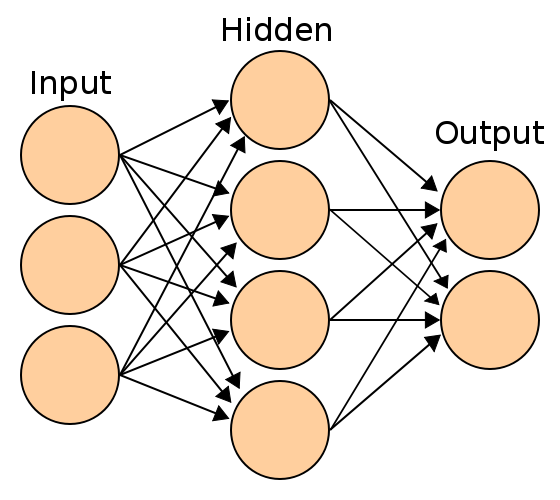
\includegraphics[width=0.5\textwidth]{artificial-neural-networks/network-layers-example.png}
    \caption{Example of a simple two-layer feedforward artificial neural network. By Colin M. L. Burnett, distributed under a CC BY-SA 3.0 license.}
    \label{fig:network-layers-example}
\end{figure}

Changing the number of layers, number of perceptrons in each layer, or the layer topologies can have huge impacts on how well the network perform, and what it can learn. Another important parameter of an \gls{ann} is the perceptrons' activation functions. The activation function determines what signal the perceptron outputs. There are countless available functions to use. The \gls{tanh} function, sigmoid function, softplus function \citep{bib:glorot2011deep}, and the \gls{relu} \citep{bib:nair2010rectified} are popular choices.

\subsection{Network structures}
\label{subsec:network-types}

There are several ways to organize the layers of an \gls{ann}, depending on what the network is trying to learn. Below is a description of two commonly used network structures that are used later in this report.

\subsubsection{\glspl{fnn}}

An \gls{fnn} is the simplest type of \gls{ann}. In an \gls{fnn}, the signals move forwards from the input through the output. Each perceptron in one layer is fully connected to all perceptrons in the subsequent layer. An example of an \gls{fnn} is shown in \cref{fig:network-layers-example}.

\subsubsection{\glspl{rnn}}

Unlike the connections in an \gls{fnn}, the connections in an \gls{rnn} can form cyclic graphs. An \gls{rnn} contains at least one feed-back connection, i.e. a connection that forms a loop. This creates an internal state of the network, allowing the network to incorporate a form of memory.

The internal memory of \glspl{rnn} make them extra useful in processing sequences of inputs, such as speech recognition.


\subsection{The training procedure}

There are several ways of training an \gls{ann}. One of the most popular training methods is called back-propagation. The method consists of two main phases: forward-propagation of input signals, and backward-propagation of error gradients.

In the forward-propagation phase, input values are fed through the input nodes and propagated through the network, generating an output. The generated output is then compared to the target output, using the \textit{loss function}. A loss function calculates the difference between the generated output and the desired output in some way. The \gls{mse} and \gls{mae} are examples of such functions.

In the backward-propagation phase, the output errors propagate backwards through the network, calculating an error gradient value for each neuron in the hidden layers. The neuron gradients are fed into the \textit{optimization function}. An optimization function adjusts the neuron weights in order to minimize the loss function. A common way of minimizing the cost function is through methods using \textit{gradient descent}. \cref{fig:gradient-descent-example} shows an example of the progression of the gradient descent method applied to a 2D function. Methods using gradient descent adjust the weights in order to "descend" the loss function towards a minimum. Popular methods utilizing gradient decent include \textit{stochastic gradient descent} \citep{bib:bottou2010large}, \textit{RMSProp} \citep{bib:hinton2012neural}, and \textit{Adam} \citep{bib:kingma2014adam}.

\begin{figure}
    \centering
    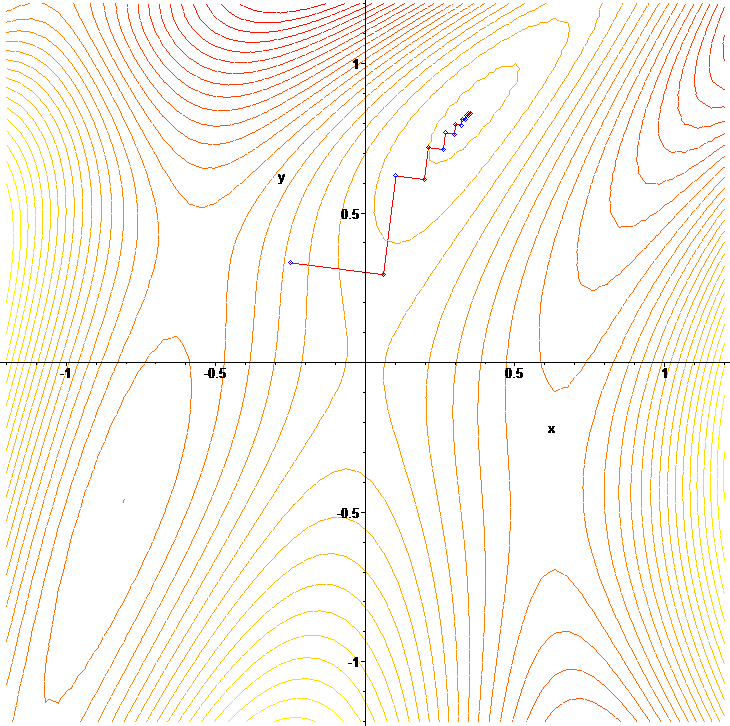
\includegraphics[width=0.7\textwidth]{artificial-neural-networks/gradient-descent-example.png}
    \caption{Example of the gradient descent method applied to a 2D function. By Joris Gillis.}
    \label{fig:gradient-descent-example}
\end{figure}

By iterating the back-propagation cycle, the weights eventually converge towards the target function. That is, if the input values are sufficient in order to describe the target function. The neurons in the hidden layers organize themselves so that they learn to recognize the patterns of the input space. Then, if a noisy, unknown observation appears, the network can respond properly if the observation contains the same underlying patterns as a training example.


\subsubsection{Dropout}

\glspl{ann} are, as other classification methods, prone to overfitting. Dropout is a widely used method for avoiding overfitting \citep{bib:srivastava2014dropout}. Using dropout, for each node, there is a probability $p$ that the node will be "deactivated", set to zero and not evaluated during training. \cref{fig:network-dropout} shows an \gls{ann} where dropout is applied.

The back-propagation method builds up co-adaptations for the training data. These adaptations do not generalize to unobserved data. Dropout breaks up these adaptations by making the presence of a specific hidden unit unreliable \citep{bib:srivastava2014dropout}.

\begin{figure}
    \centering
    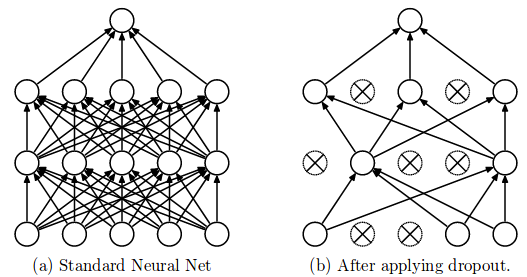
\includegraphics[width=0.7\textwidth]{artificial-neural-networks/dropout.png}
    \caption{Graphical illustration of the effects of dropout. Taken from \citet{bib:srivastava2014dropout}.}
    \label{fig:network-dropout}
\end{figure}

%========================================================================
%   CHAPTER: SYSTEM ARCHITECTURE
%========================================================================

\chapter{System architecture}
\label{chp:system-architecture}
This chapter presents a description of the architecture of the system used for gathering and evaluating data used in this report.
\section{Database overview}
\label{sec:database-overview}

To be able to use the data available at \whoscored\ for training an \gls{ann}, it should be stored on a computer data storage device in some way. As there are vast amounts of available data, and the data is highly connected, a good option is to store the data in a relational database. Relational databases are designed with relational models in mind, and is therefore a natural choice of storage. 

This section describes the database used for storing the data used in this report. The database is set up using MySQL version 5.7.


\subsection{Central data}

\cref{fig:database-central} shows the five most central database tables.

A \textit{region} is either a nation, continent, or \textit{International}. International covers tournaments spanning several continents, such as the FIFA World Cup. Continents cover tournaments spanning several countries within the same continent, such as the UEFA European Championship. Nations cover national tournaments, such as the English Premier League. Nations are also used for tracking the nationality of club teams and players.

A \textit{league} is a tournament, either a league or a knockout tournament. A tournament spans over several \textit{seasons}, given by the year the season starts. This makes it possible to differentiate two seasons from each other, such as the 2015-2016 and 2016-2017 seasons of the English Premier League.

A \textit{team} is either a club or national team. Teams are not directly connected to any leagues, as teams can be promoted or relegated.

A \textit{player} is a former or present football player. Players are not directly connected to any teams, as players may change team.

\begin{figure}
    \centering
    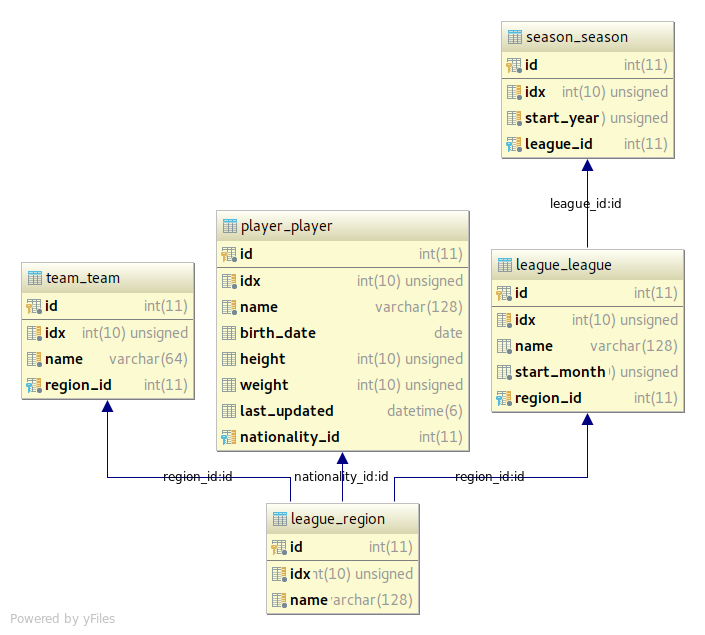
\includegraphics[width=0.9\textwidth]{database/central.png}
    \caption{Most central database tables.}
    \label{fig:database-central}
\end{figure}


\subsection{Matches}
\label{subsec:database-overview-matches}

\cref{fig:database-matches} shows the database tables containing information concerning matches.

A \textit{match} is a single match between two teams, the \textit{home team} and the \textit{away team}. Matches are played at a specific \textit{venue}, and is conducted by a specific \textit{referee}. All matches are part of a \textit{season}. Matches can be \textit{sparse}, meaning that they are covered by a minimum or intermediate level of details. Complete matches are marked with the Boolean attribute \textit{complete}. Matches that are postponed are marked with the \textit{postponed} attribute. For speeding up data fetching, two attributes, \textit{last\_matches\_fetched} and \textit{previous\_matches\_fetched}, marks whether the \textit{last matches} for the two teams, and the \textit{previous matches} between the teams have been fetched.

A \textit{previous meetings} instance lists the previous meetings between the two competing teams of a match. Previous meetings instances list a summary of the number of victories, goals scored, and cards issued for the two teams. For each match, there are three sets of previous meetings: one for the most recent matches, one for the most recent matches played at the home team venue, and one for the most recent matches played at the away team venue. These three sets are stored in the \textit{head to head} table.

It is possible to store a set of \textit{match odds} for a match. A match odds instance lists the odds for the three match outcomes (home victory, draw, or away victory) offered by a given \textit{bookmaker}.

\begin{figure}
    \centering
    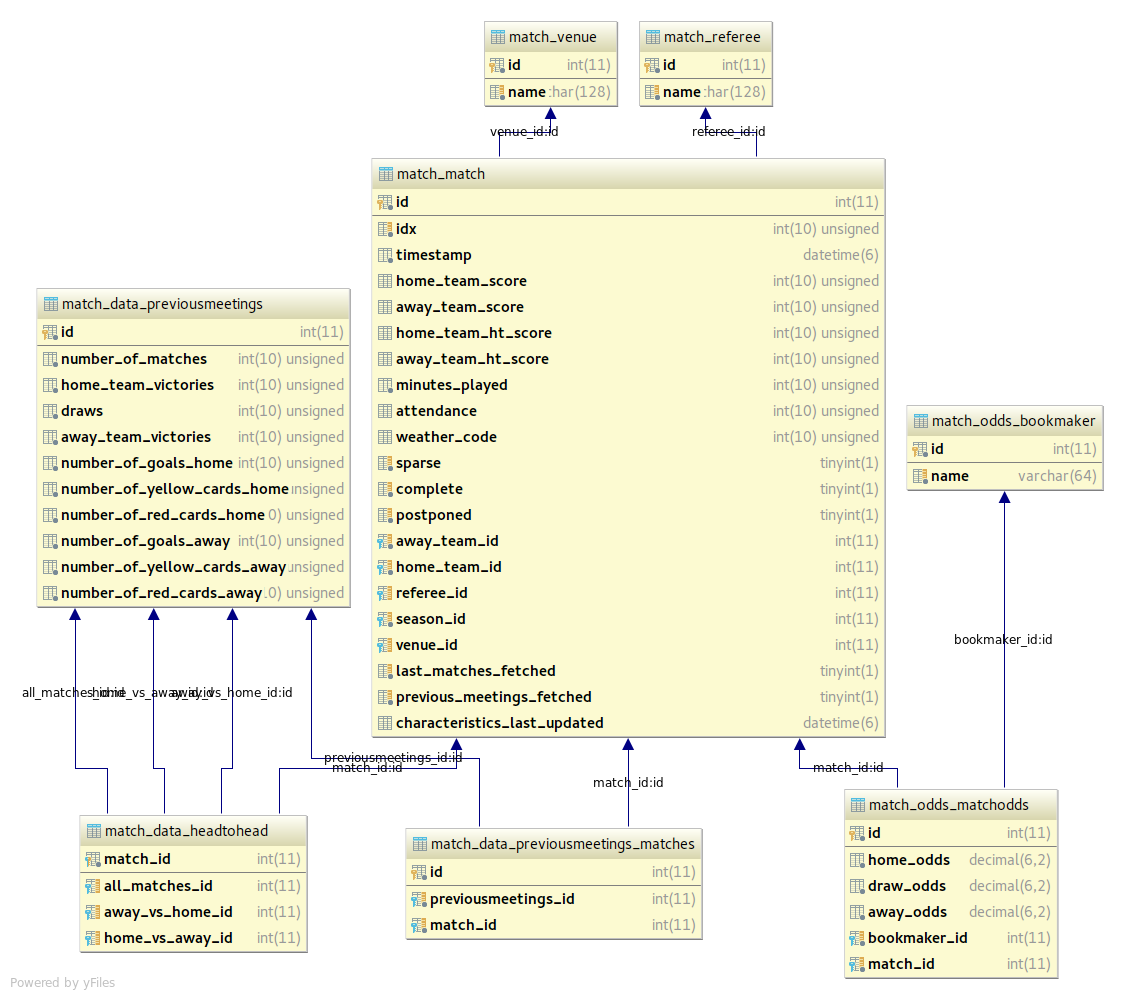
\includegraphics[width=0.9\textwidth]{database/match.png}
    \caption{Database tables containing match related information.}
    \label{fig:database-matches}
\end{figure}


\subsection{Team stats}
\label{subsec:database-overview-team-stats}

\cref{fig:database-team-stats} shows the database tables containing information concerning team stats.

A \textit{team stats} instance contains information concerning a team's participation in a match. For each match, there are two team stats, one for the home team, and one for the away team. A fully detailed team stats instance contains sets of \textit{ratings} and \textit{statistics}, developed over time, in addition to a final rating. Team ratings are sampled almost every minute and stored in the ratings set. The statistics contains a set for every metric in \cref{tab:whoscored-player-metrics}.

Each team stats instance has a set of associated \textit{team characteristics}. Characteristics are given by a type (offensive or defensive) and a name. A characteristic is either a strength, a weakness, or a style. Strengths and weaknesses have associated levels, ranging from 15 (very weak) to 55 (very strong).

\begin{figure}
    \centering
    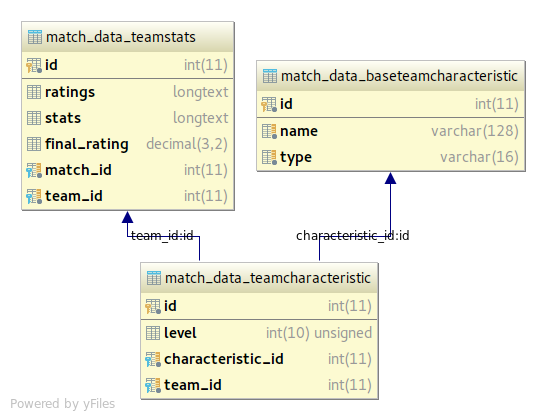
\includegraphics[width=0.9\textwidth]{database/team-stats.png}
    \caption{Database tables containing team stats related information.}
    \label{fig:database-team-stats}
\end{figure}


\subsection{Player stats}

\cref{fig:database-player-stats} shows the database tables containing information concerning player stats.

A \textit{player stats} instance contains information concerning a player's participation in a match. For each match, there are at least 22 player stats, one for each player. For matches with intermediate or full level of details, substitutes are also included. Player stats instances are marked with \textit{minute started} and \textit{minute ended}, marking what parts of the game the player participated in. A fully detailed player stats instance contains \textit{ratings} and \textit{statistics}, similar to those for team stats. In addition, player stats instances contain the final count for every metric in \cref{tab:whoscored-player-metrics}. Player stats are marked with two Boolean values, \textit{is\_first\_eleven} and \textit{is\_man\_of\_the\_match}, signaling whether the player started the match or was rated man of the match, respectively. A player stats instance is also associated with a \textit{player position}, such as \textit{goal keeper}, \textit{left back}, etc.

\textit{Player characteristics}, are not associated with a specific match, but rather with the player object itself.

\begin{figure}
    \centering
    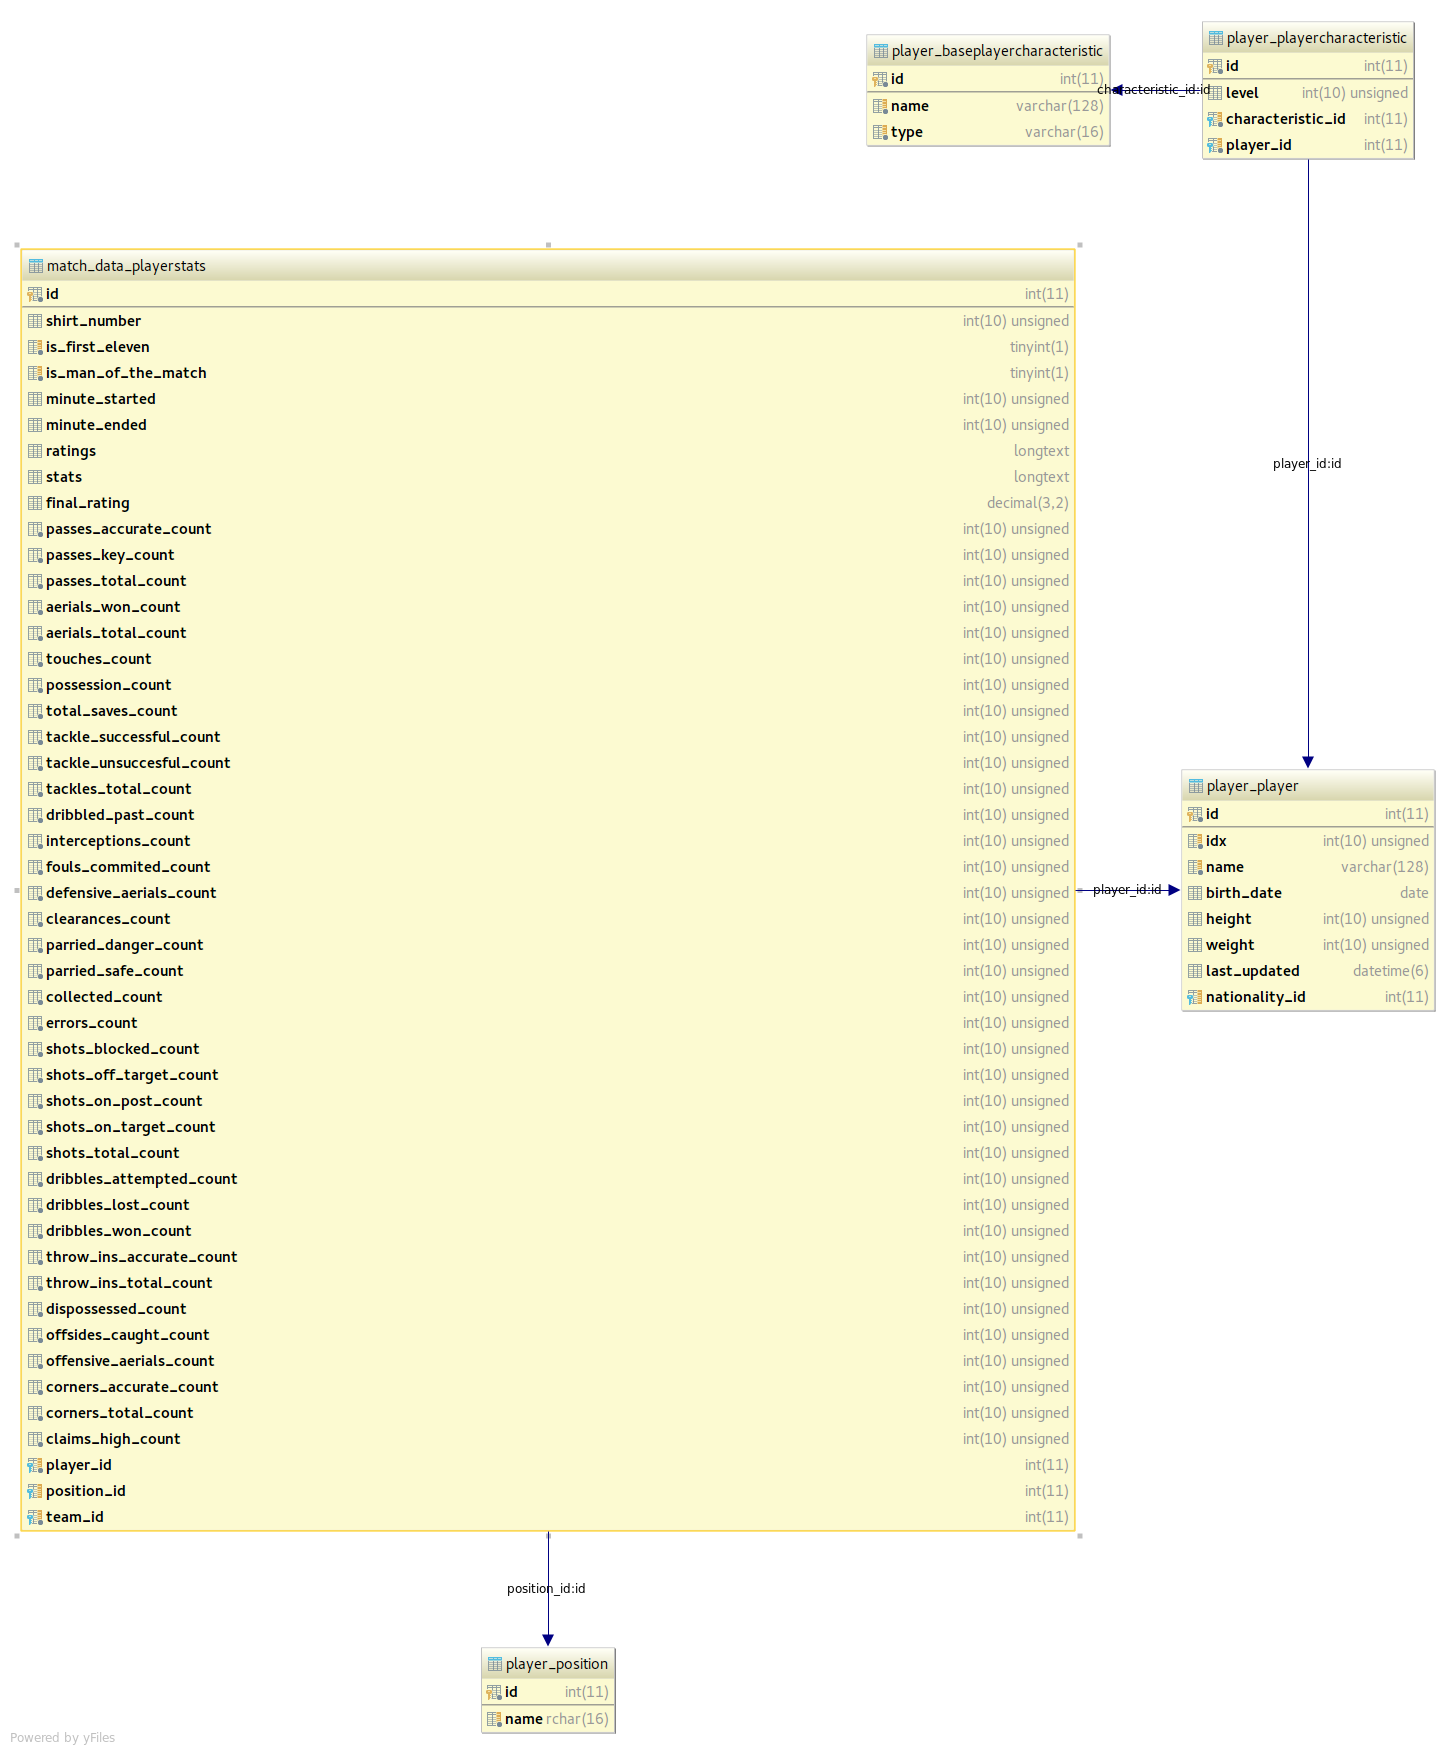
\includegraphics[width=0.9\textwidth]{database/player-stats.png}
    \caption{Database tables containing player related information.}
    \label{fig:database-player-stats}
\end{figure}


\subsection{Events}

\cref{fig:database-events} shows the database tables containing information concerning match events.

The \textit{event} table covers almost everything that takes place on the pitch during a match. An event is of a specific \textit{event type}, as listed in \cref{tab:whoscored-event-types}. An event takes place at specific \textit{position} on the pitch, at a given \textit{time} during the match. Most events are executed by a \textit{player} for one of the competing \textit{teams}. Some events, such as \textit{goals} and \textit{missed shots}, have related events. Events are marked with four Boolean attributes, \textit{is\_touch}, \textit{is\_goal}, \textit{is\_own\_goal}, \textit{is\_shot}. Events that span an area (such as shots, passes, etc.) are marked with an \textit{end position}. Events that enter the goal are marked with a \textit{goal position}, marking where it passed the goal mouth.

An event has a set of \textit{qualifiers}. Qualifiers describe the event in details. A qualifier is of a specific \textit{type}. \textit{Corner taken}, \textit{key pass}, \textit{angle}, \textit{length}, \textit{zone}, \textit{goal kick}, \textit{parried danger}, and \textit{hands} are some examples of qualifier types. Qualifiers such as \textit{angle}, \textit{length}, and \textit{zone} have associated \textit{values}. 

\begin{figure}
    \centering
    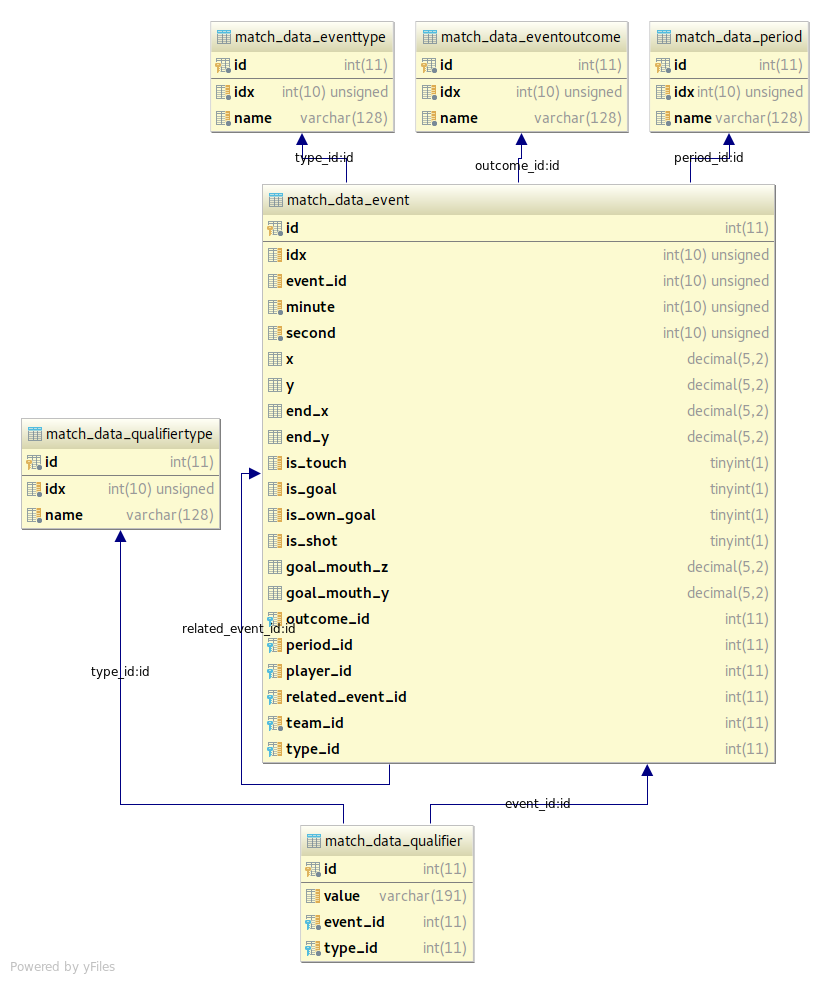
\includegraphics[width=0.9\textwidth]{database/event.png}
    \caption{Database tables containing event related information.}
    \label{fig:database-events}
\end{figure}


\subsection{Formations}

\cref{fig:database-formations} shows the database tables containing information concerning team formations.

\textit{Team formations} are included in matches with full level of details. A team formation concerns a specific \textit{team's} setup during a specific \textit{interval} of a match. Team formations have associated \textit{team captains}. A new team formation is created every time a team makes a substitution or rotates \textit{player positions}. A player position concerns a single player, and where on the pitch he plays at the given team formation.

Each team formation has an associated \textit{formation}. A formation signals how the players are arranged (4-4-2, 4-3-1, etc.).

\begin{figure}
    \centering
    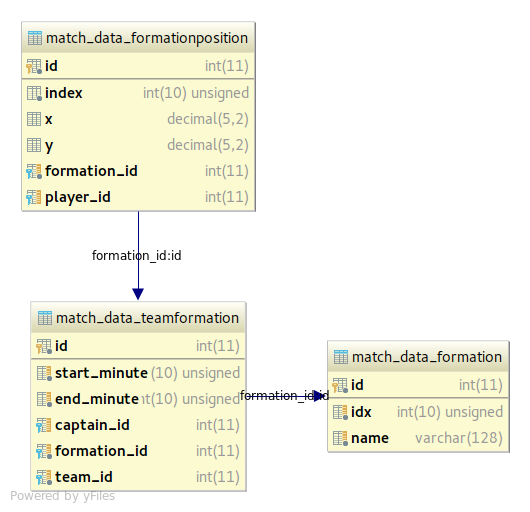
\includegraphics[width=0.9\textwidth]{database/formation.png}
    \caption{Database tables containing formation related information.}
    \label{fig:database-formations}
\end{figure}


\subsection{Substitutions}

\cref{fig:database-substitutions} shows the database tables containing information concerning substitutions.

Every time a player is substituted, a \textit{substitution} instance is created. A substitution contains information about what players were substituted at what time and period of the match.

\begin{figure}
    \centering
    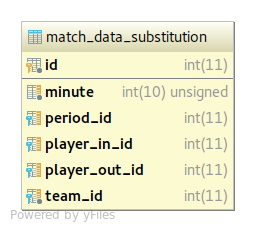
\includegraphics[width=0.5\textwidth]{database/substitution.png}
    \caption{Database table containing substitution related information.}
    \label{fig:database-substitutions}
\end{figure}
\section{\whoscoredplain\ crawler}

There are several steps one must go through in order to populate the database in \cref{sec:database-overview}. For each season, one must first gather the IDs for all the matches. When the IDs are gathered, one can start traversing all matches, gathering scorelines, event information, player statistics, etc. Below comes a description of how to locate the different data sources, and how to extract the data.


\subsection{URL structure}

When crawling \whoscored\  for data, one must know where the web pages containing the wanted data are located. Every match, team, and player listed on \\ \whoscored\ has its own unique ID, given as an integer number. Regions, leagues, seasons, and season stages also has their own unique IDs. Different entity types have their own URL structure. The only difference between the URLs of two entities of the same kind are their IDs.


\subsection{Match IDs}

Season fixtures are available at the following URLs:

\whoscoredurl{/Regions/REGION/Tournaments/TOURNAMENT/Seasons/SEASON/Stages/STAGE/Fixtures},

where \textbf{REGION} is the region of the tournament, \textbf{TOURNAMENT} the tournament in question, \textbf{SEASON} the season to fetch fixtures for, and \textbf{STAGE} the stage of the season. For league tournaments, the stage ID stays the same. For knockout tournaments, there are different stages per season (qualification, group stage, and knockout stage). The example below points to the fixture list for the English Premier League 2016-2017:

\whoscoredurl{/Regions/252/Tournaments/2/Seasons/6335/Stages/13796/Fixtures},

where 252 is the region ID for England, 2 the tournament ID for the English Premier League, 6335 the season ID for the English Premier League 2016-2017, and 13796 the stage ID for the season.

Fixtures are grouped by year and month. Finished matches are marked with the final score, while coming matches are marked with "\textbf{vs}". The matches are listed in a large table, with one row for each match, as shown in \cref{fig:whoscored-fixture-list}.

\begin{figure}
    \centering
    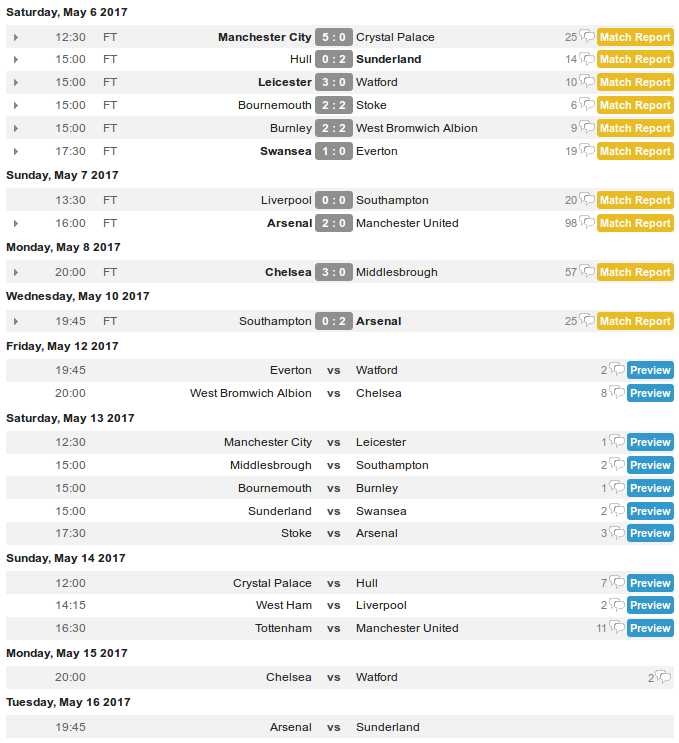
\includegraphics[width=0.9\textwidth]{whoscored/fixture-list.png}
    \caption{Small portion of the match fixtures for English Premier League, May 2017.}
    \label{fig:whoscored-fixture-list}
\end{figure}

The row elements contain the ID for each match. Extracting the match ID is as simple as fetching the \url{data-id} attribute from the row element. The example below shows the row element for Arsenal versus Manchester United May 7, 2017.
\begin{lstlisting}[language=HTML,caption={Hypertext to Arsenal versus Manchester United May 7, 2017.}]
<tr class="item" data-id="1080862">...</td>
\end{lstlisting}


\subsection{Match data}

Match URLs are of the following form:

\whoscoredurl{/Matches/ID/VIEW},

where \textbf{ID} is the match ID, and \textbf{VIEW} is the view. A match has several views, depending on whether it is detailed or not, and whether it is finished, ongoing or not started. The different views are listed in \cref{tab:whoscored-match-views}. The example below points to the \url{Live} view showing detailed match event information for Arsenal versus Manchester United May 7, 2017.

\whoscoredurl{/Matches/1080862/Live}

\subsubsection{Match events}

Match event data is located at the \url{Live} match view. Event data is stored in three different locations, depending on detail level. All match event data is located in JavaScript variables in the source code of the respective web page. Fetching the data can easily be done using simple regular expressions.

The minimum match details are located in a variable called \textit{matchHeader}. A description of the data in the match header is shown in \cref{tab:whoscored-match-header-data}. The example below is from Arsenal versus Manchester United May 7, 2017.
\begin{lstlisting}[language=JavaScript,caption={Match header from Arsenal versus Manchester United May 7, 2017.}]
matchHeader.load([13,32,'Arsenal','Manchester United','07/05/2017 16:00:00','07/05/2017 00:00:00',6,'FT','0 : 0','2 : 0',,,'2 : 0','England','England']);
\end{lstlisting}
13 and 32 are the team IDs of Arsenal and Manchester United, respectively. The match started at "07/05/2017 16:00:00". The status code 6 indicates that the match is complete. FT indicates that the match was ended at full time. No goals were scored during the first half. Arsenal won the match 2-0. Both teams are located in England.

Extracting the match header from the web page source code can be done using the following regular expression:
\begin{lstlisting}[language=Python,caption={Regular expression used to extract match header data.}]
    /matchHeader\.load\((.+?)\);/
\end{lstlisting}

The intermediate match details are located in a variable called \textit{initialMatchDataForScrappers} \textit{[sic]}. The variable contains the match header, lineups, substitutions and most important match events. Extracting the intermediate match details from the web page source code can be done using the following regular expression:
\begin{lstlisting}[language=Python,caption={Regular expression used to extract initialMatchDataForScrappers.}]
    /var initialMatchDataForScrappers = (.+?);/
\end{lstlisting}

The full match details are located in a variable called \textit{matchCentreData}. The variable is divided into three main parts: general information, home team information, and away team information. The included information is described in \cref{subsec:whoscored-match-details}. Extracting the full match details from the web page source code can be done using the following regular expression:
\begin{lstlisting}[language=Python,caption={Regular expression used to extract matchCentreData.}]
    /var matchCentreData = (.+?);/
\end{lstlisting}


\subsubsection{Head to head information}

Head to head information is located at the \url{Show} match view.

Previous meetings (up to six matches) between the two teams are listed in a table, with one row for each match, as shown in \cref{fig:whoscored-previous-meetings}. For each match, there is a hypertext to the match web page.
\begin{figure}
    \centering
    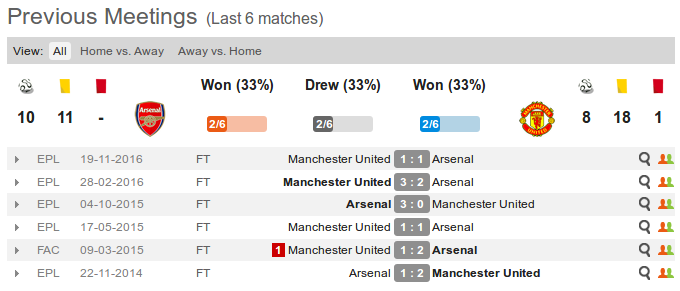
\includegraphics[width=\textwidth]{whoscored/previous-meetings.png}
    \caption{Previous meetings between Arsenal and Manchester United before the match May 7, 2017.}
    \label{fig:whoscored-previous-meetings}
\end{figure}

The example below is from Arsenal versus Manchester United May 7, 2017, showing a hypertext to their last meeting.
\begin{lstlisting}[language=HTML,caption={Hypertext to the last meeting before the match between Arsenal and Manchester United May 7, 2017.}]
    <a class="..." href="/Matches/1080633/Live/England-Premier-League-2016-2017-Manchester-United-Arsenal">1 : 1</a>
\end{lstlisting}
One can extract the match ID from the hypertext using the following regular expression on the hypertext URL:
\begin{lstlisting}[language=Python,caption={Regular expression used to extract match ID from hypertext.}]
    /Matches/(\d+)/
\end{lstlisting}

Previous matches (also up to six matches) for the two teams are listed in the same way.

Team characteristics for the two teams are listed as three different sets of characteristics: strengths, weaknesses, and styles. All characteristics are given a textual description. Strengths and weaknesses are also given indications of their levels (very weak, weak, strong, very strong).
\begin{figure}
    \centering
    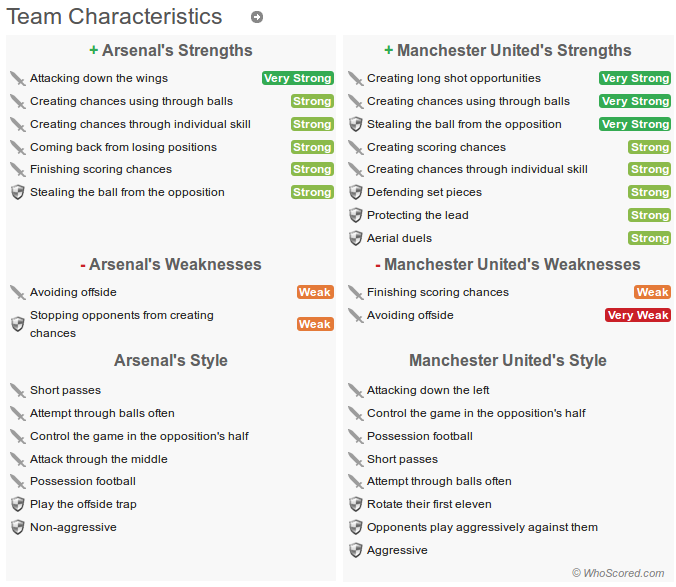
\includegraphics[width=\textwidth]{whoscored/team-characteristics.png}
    \caption{Team characteristics for Arsenal and Manchester United before the match May 7, 2017.}
    \label{fig:whoscored-team-characteristics}
\end{figure}

\clearpage
\section{Neural networks}

During the experiments conducted in this report, several \glspl{ann} have been explored. As almost all the different networks had the same basic structure, with identical loss functions, optimizer functions, accuracy measures, data sources, etc., the need to re-use the source code soon emerged. To solve this, an abstract network class supporting all the basic functionality was constructed. The abstract network class was implemented with modularity, extensibility, customizability, and ease of use in mind. 

\subsection{The abstract network class}

The abstract network class contains all the basic functionality needed in order to train and evaluate an \gls{ann}, along with procedures to fetch pre-trained models and use them for prediction of new observations. The abstract network class takes care of everything not problem specific, such as generating training, validation, evaluating, and prediction data sets, storing and handling trained models, storing data sets, etc. 

The abstract network class uses Keras to handle its network functionality. Keras supplies functionality for constructing, training, and evaluating \glspl{ann}. Keras also supplies functionality for storing and accessing trained models. These models (called model checkpoints) can easily be used for prediction the labels of new observations.

All the different properties of the network class are implemented as functions. By extending the abstract network class, one can easily override the functions to customize the network.

\subsubsection{Network name}

As each network generates its own data set and checkpoints, there is a need to distinguish one network from another. Each network implemented is therefore given an unique name, describing its function. An example is the network \textit{head-to-head-home-to-result}, that predicts match result given the head to head information for the match.

When each network has its own unique identifier, it is easy to store data sets and checkpoints in separate folders. In addition, Keras supports naming the network layers. Each layer in the network needs an unique name. For supporting networks as combination of other networks, all layer names are prefixed with the network name.

\subsubsection{Loss function}

Most of the \glspl{ann} used in the experiments map some input data to a probability distribution for the three possible match outcomes (home victory, draw, away victory). The loss function is therefore set to \textit{sparse categorical crossentropy} as default. Sparse categorical crossentropy is used for categorical classifying, i.e. for assigning a class to an observation, and not for approximating a real numbered value. When using the sparse categorical crossentropy, labels are given as integers. It is then an easy task assigning a label to a match: 0 for home victory, 1 for draw, 2 for away victory.

\subsubsection{Optimizer}

The optimizer is set to Adam \citep{bib:kingma2014adam} as default. Adam is an adaptive optimizer function that offers some extensions to another popular optimizer: RMSProp \citep{bib:hinton2012neural}. Both Adam and RMSProp compute adaptive learning rates, but Adam also utilizes an exponentially decaying average of gradients, similar to a momentum.

\subsubsection{Network layers}

One thing that differs between the networks is the network topology. Most networks have different hidden layer topologies. Therefore, the function that defines the hidden layers must be implemented for each network.

Input data shapes also differ from network to network. The function for defining the network's input layer is implemented, but an own function defining the input data shape is not. Each network defines its own input data shape, and the input layer is generated based on the shape.

The output layer is also defined in an own function. Almost all networks have the same output layer: a fully connected layer of three nodes, activated by the softmax function. The softmax function squeezes a K-dimensional vector of real values into K-dimensional vector of real values in the range $[0, 1]$. The values in the output vector sum to $1$. This makes the softmax function exceptional for probability distributions.

\subsubsection{Setting up the network model}

When the above properties are implemented, the network is ready for model training and outcome prediction.

The input layer is set up as model input. The hidden layers are then iterated and added to the model. Then, the output layer is added. Lastly, the model is set up to use the loss function and optimizer specified.

\subsubsection{Generating input data}

Each network has an unique mapping from match instance to model input data. The function for generating input data must therefore be implemented for each network. However, procedures for storing input data are included in the abstract network class. Storing the input data instead of generating it each time training the network saves quite a lot of time.


\subsubsection{Storing and handling trained models}

Every time a network is trained, the results are stored by the abstract network class. Each training run is assigned its own folder on the file system.

Keras has implemented a callback function called \textit{ModelCheckpoint}. This callback function allows for storing model checkpoints during training. The callback function allows for storing only the best model checkpoint (every time the loss value of the validation data set reaches a new minimum). Resorting the checkpoint file is then easily done using Keras' API.

\subsubsection{Storing and handling data sets}

Every time the abstract network class encounters a new match instance, it generates the corresponding model input data. If the match is complete, the input data is added to a dictionary, with the match ID as key. The dictionary is then stored in a file for future use.

If the network encounters a known match, it can simply fetch the model input from the dictionary instead of generating it again.

\subsubsection{Training}

The abstract network class has an own procedure for training the model. The training procedure sets up the network model using the specified topology, loss function, and optimizer. Training data and validation data are then generated using the model input data generation function. The model is then fitted to the training data, and cross validated using the validation set. The training procedure returns the model checkpoint with lowest validation loss.

The training procedure itself is customizable. The number of training epochs and batch size can be changed using run-time arguments. What matches to include in the training data set can also be changed using run-time arguments.

\subsubsection{Evaluating}

The abstract network class also has a procedure for evaluating the model. What season to evaluate is set using run-time arguments. The matches for the given season are fed to the model, and the resulting prediction accuracy is shown. The minimum, maximum, and mean \gls{rps} values are also shown.

\subsubsection{Predicting}

Lastly, the abstract network class has a procedure for predicting match instances. Specific matches to predict can be set using run-time arguments. It is also possible to predict all matches in an entire season. For each match, the probability distribution for the three outcomes are shown.


\subsection{Extending the abstract network class}

To construct a valid \gls{ann} using the abstract network class, one must create a class that extends the abstract network class. Four properties must be implemented: network name, model input data shape, hidden network layers, and model input data generation function.

When these four properties are implemented, training and evaluating the model, and predicting the label of new observations can easily be done by instantiating the network class and calling the respective functions on the instance.

\subsubsection{Example using the head-to-head-home-to-result network}

\cref{lst:head-to-head-example} shows the complete class for the head-to-head-home-to-result network. The network takes takes a summary of the recent matches between the teams as model input. The network is further explained in \cref{subsec:head-to-head}.

The \textit{\_\_init\_\_} function takes in the run-time arguments. These arguments are used for generating training, evaluation, and prediction data, and when training the model.

The static function \textit{name} simply returns the name of the network.

The function \textit{input\_shape} defines the shape of the model data. Each match is mapped to a list of five floating point numbers.

The function \textit{default\_layers} defines the hidden layers of the model. The model consists of a single hidden layer, with 32 nodes. The hidden layer is activated using the sigmoid function.

The function \textit{input\_function} maps a match to model input data. Input model data consist of a set of features and a label for each match. A summary of the most recent matches between the teams at the home team venue is fetched. If no such summary exists, the match is skipped, as it does not have the sufficient data for training or predicting. The distributions of match outcomes and goals scored are added as the match's features. The final result is the label of the match.

\begin{lstlisting}[language=Python,caption={The head-to-head-home-to-result network class.},label={lst:head-to-head-example}]
class HeadToHeadHomeToResultNetwork(AbstractNetwork):
    def __init__(self, args, layers=None):
        super().__init__(args, layers)

    @staticmethod
    def name():
        return 'head-to-head-home-to-result'

    @property
    def input_shape(self):
        return 5,

    @property
    def filters(self):
        super_filters = super().filters

        super_filters.update({
            'previousmeetings__isnull': False,
        })

        return super_filters

    @property
    def default_layers(self):
        return [
            Dense(32, activation='sigmoid'),
        ]

    def input_function(self, match, training_data=True):
        summary = match.previous_meetings.home_vs_away

        if summary is not None:
            return [*summary.victory_distribution, *summary.goal_distribution], match.final_result
\end{lstlisting}
\section{Betting simulator}

To test the profitability of the prediction models evaluated in this report, a betting simulator was created.

The betting simulator simulates one season of a given tournament. The matches for the given season are grouped into ordered game weeks, like in real life. Odds from several bookmakers are considered when deeming bets feasible, and when placing bets.

Each simulation starts with a given bankroll. \cref{alg:betting-simulation-procedure} shows the steps taken during the betting simulation.
\begin{algorithm}
    \caption{Betting simulation procedure \label{alg:betting-simulation-procedure}}
    set bankroll, $C$, to initial bankroll size\;
    \For{game week $\in$ season}{
        \For{match $\in$ game week}{
            calculate match outcome probability distribution\;
            \For{outcome $i \in \{0, 1, 2\}$}{
                fetch all available odds for outcome $i$, $d_{ij}$, from bookmakers $j \in \{1, ..., N\}$\;
                find the highest odds, $max\{d_{ij}\}$, and the bookmaker $j$ offering it\;
                calculate the mean odds, $\overline{d_{ij}}$\;
                \If{bet is feasible, that is $\overline{d_{i}} * P_{i} > 1 + \tau$}{
                    place bet of size $c_{i}$ at bookmaker $j$ offering the highest odds\;
                    update bankroll, removing bet size, $C = C - c_{i}$\;
                }
            }
        }
        \For{placed bets}{
            \If{bet is successful}{
                update bank roll, adding gain from bet, $C = C + d_{ij} * c_{i}$
            }
        }
    }
\end{algorithm}

According to the findings of \citet{bib:vlastakis-dotsis-markellos-2009}, the European betting marked is inefficient. That is, some bookmakers offer unreasonable high odds, not representative of the overall betting market. This is the reason why mean odds are considered when deeming bets feasible.

%========================================================================
%   CHAPTER: EXPERIMENTAL SETUP
%========================================================================

\chapter{Experimental setup}
\label{chp:experimental-setup}
This chapter presents the setup for the experiments conducted in this report. The chapter first presents a description the prediction models. A presentation of the betting simulation procedure is then presented.
\section{Prediction models}
\label{sec:prediciton-models}

This section presents the different networks constructed for training prediction models. For each network, the model input is presented, along with a rationale behind the network.

When measuring the performance of a network, different network configurations are evaluated. For each configuration, ten different prediction models are trained. At each training round, the initial weights and biases of the network are randomized, making sure no two models are the same. In addition, the training data set is scrambled randomly before each training round. By doing this, the results present the overall accuracy of the network, and not just the effects of a potentially lucky combination of initial weights and training data.

For each configuration, the minimum, maximum, and mean \gls{rps} values are presented. In addition, the prediction accuracy of the model is presented.

Prediction accuracy is evaluated for the 2015-2016 season of the English Premier League. The most promising configuration for each network is then used for evaluating the profitability of the prediction models over the span of the seasons 2015-2017 of the English Premier League. The 2016-2017 season is not included when measuring prediction accuracy, to give a more realistic betting simulation. The results are not that credible if one choose network configuration based on the same data for which the model will be evaluated.

When training the prediction models, matches all the way back to the 2009-2010 season of the English Premier League are used. This is the first season where \\ \whoscored\ offered fully detailed match information. As the data available at \whoscored\ is not perfect, matches with incomplete data are excluded from training.
\subsection{Player ratings}

The player ratings provided by \whoscored\ are calculated using over 200 statistics, and provide an accurate measure on a player's contributions to the team \\ \citep{bib:whoscored-ratings}. The player ratings are adjusted throughout the whole match. Every event of importance is taken into account when calculating the rating.

Before using player ratings for predicting match outcome, one should confirm that the ratings actually have predictive properties. To confirm this, a simple \gls{fnn} with one hidden layer of 64 nodes, activated using \gls{relu} was set up. The network takes in the final rating of the 22 starting players for each match. \cref{fig:network-player-ratings-to-result} shows the network structure. 

The input values $I_{1}, ..., I_{22}$ are the final ratings for the 22 starting players, divided by $10$ to map them to the range $[0, 10]$. The players are first ordered by team. The first 11 input values are players from the home team, and the next 11 are from the away team. The players in each team are also ordered, first by $x$ position on the field, then by $y$ position on the field. The position $(0, 0)$ is at each team's right corner flag. This makes the keeper the first player, and the forwards the last.

For the match between Arsenal and Manchester United May 7, 2017, shown in \cref{fig:arsenal-manchester-united-player-ratings}, the input values would be as follows:
\begin{lstlisting}[language=Python]
    [0.76, 0.70, 0.74, 0.68, 0.81, 0.72, 0.75, 0.73, 0.72, 0.70, 0.77, 0.60, 0.67, 0.62, 0.65, 0.66, 0.65, 0.67, 0.61, 0.69, 0.66, 0.65]
\end{lstlisting}

\begin{figure}
    \centering
    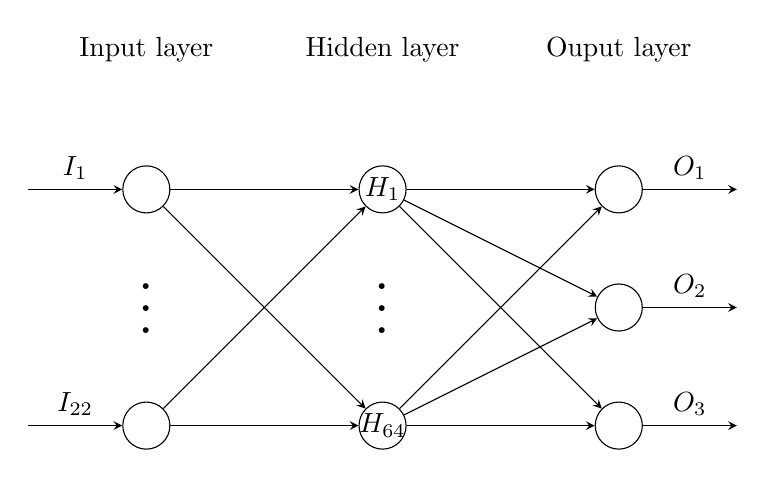
\begin{tikzpicture}[x=1.5cm, y=1.5cm, >=stealth]
        %%%%%%%%%%%%%%%%%%%%%%%%%%%%%%%%%%%%%%%%%%%%
        % Input nodes
        %%%%%%%%%%%%%%%%%%%%%%%%%%%%%%%%%%%%%%%%%%%%
        
        % Drawing
        \foreach \m/\l [count=\y] in {1,missing,2}
            \node [every neuron/.try, neuron \m/.try] (input-\m) at (0,2-\y) {};

        % Labeling
        \foreach \l [count=\i] in {1,22}
            \draw [<-] (input-\i) -- ++(-1,0)
                node [above, midway] {$I_{\l}$};
        
        
        %%%%%%%%%%%%%%%%%%%%%%%%%%%%%%%%%%%%%%%%%%%%
        % Hidden nodes
        %%%%%%%%%%%%%%%%%%%%%%%%%%%%%%%%%%%%%%%%%%%%
        
        % Drawing
        \foreach \m [count=\y] in {1,missing,2}
            \node [every neuron/.try, neuron \m/.try ] (hidden-\m) at (2,2-\y) {};
        
        % Labeling
        \foreach \l [count=\i] in {1,64}
            \node at (hidden-\i) {$H_{\l}$};
        
        
        %%%%%%%%%%%%%%%%%%%%%%%%%%%%%%%%%%%%%%%%%%%%
        % Output nodes
        %%%%%%%%%%%%%%%%%%%%%%%%%%%%%%%%%%%%%%%%%%%%
        
        % Drawing
        \foreach \m [count=\y] in {1,...,3}
            \node [every neuron/.try, neuron \m/.try ] (output-\m) at (4,2-\y) {};
        
        % Labeling
        \foreach \l [count=\i] in {1,...,3}
            \draw [->] (output-\i) -- ++(1,0)
                node [above, midway] {$O_{\l}$};
        
        
        %%%%%%%%%%%%%%%%%%%%%%%%%%%%%%%%%%%%%%%%%%%%
        % Connecting
        %%%%%%%%%%%%%%%%%%%%%%%%%%%%%%%%%%%%%%%%%%%%
        
        % Input nodes to hidden nodes
        \foreach \i in {1,...,2}
            \foreach \j in {1,...,2}
                \draw [->] (input-\i) -- (hidden-\j);
        
        % Hidden nodes to output nodes
        \foreach \i in {1,...,2}
            \foreach \j in {1,...,3}
                \draw [->] (hidden-\i) -- (output-\j);
        
        
        %%%%%%%%%%%%%%%%%%%%%%%%%%%%%%%%%%%%%%%%%%%%
        % Labeling layers
        %%%%%%%%%%%%%%%%%%%%%%%%%%%%%%%%%%%%%%%%%%%%
        \foreach \l [count=\x from 0] in {Input, Hidden, Ouput}
            \node [align=center, above] at (\x*2,2) {\l\ layer};
    \end{tikzpicture}
    \caption{Player ratings network structure.}
    \label{fig:network-player-ratings-to-result}
\end{figure}

\begin{figure}
    \centering
    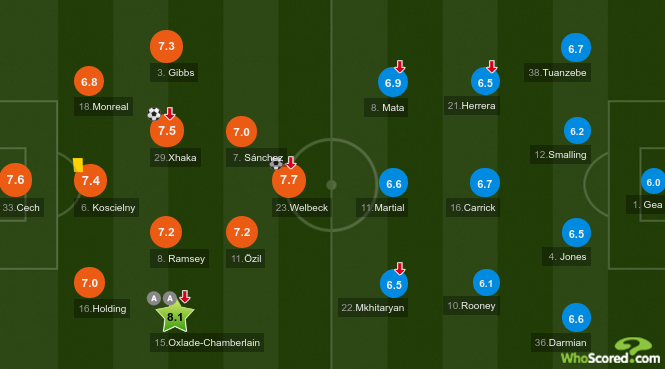
\includegraphics[width=\textwidth]{experimental-setup/arsenal-manchester-united-player-ratings.png}
    \caption{The final ratings for the players starting the match between Arsenal and Manchester United May 7, 2017.}
    \label{fig:arsenal-manchester-united-player-ratings}
\end{figure}

The network can with $90\%$ certainty predict the match outcome (averaged over ten network instances), yielding an average \gls{rps} of $0.0394$. This indicates the player ratings say a lot about the final rating.

\subsubsection{Input}

As the final ratings are not known at match start, ratings from previous matches must be used. For each starting player, the three most recent matches are taken into consideration. The following values from the three previous matches of each player are added to the model input:
\begin{itemize}[noitemsep]
    \item Player's final rating.
    \item Portion of the match played: The number of minutes played divided by $120$. This is added in order to increase the impact of players playing the whole match. 120 is used instead of 90 to support matches that might go to extra time.
    \item Player's team's final rating. This is added to capture cases where the player rating are affected by of the team's collective effort.
    \item Other team's final rating. This is added to capture cases where the player rating are affected by of the other team's collective effort.
    \item A Boolean value, indicating whether the player played at home or away. This is added to take the home ground advantage into consideration.
    \item Days since the match, $exp(-\text{days since match} / 7)$. This is added in order to increase the impact of more recent matches.
\end{itemize}

In addition to the previous match features, the number of matches the last two game weeks are added for each player. That gives $3 * 6 + 1 = 19$ features for each player. With $22$ players, there are $22 * 19 = 418$ features per match.
\subsection{Head to head}
\label{subsec:head-to-head}

The idea behind this network is to capture match history and the home ground advantage. The network is inspired by the earlier works presented in \cref{sec:background-models}.


\subsubsection{Input}

The network takes in a \textit{PreviousMeetings} (see: \cref{subsec:database-overview-matches}) object containing information about the last matches played at the home team ground.

For each match, the following values are added to the model input:
\begin{itemize}[noitemsep]
    \item Distribution of outcomes over the previous registered matches. For each of the three outcomes, the number of occurrences of the outcome is divided by the total number of matches.
    \item Distribution of goals over the previous registered matches. The number of goals scored by the home team, divided by the total number of goals scored, and the number of goals scored by the away team, divided by the total number of goals scored.
\end{itemize}

For the match between Arsenal and Manchester United May 7, 2017, the input values would be as follows:
\begin{lstlisting}[language=Python]
    [1/3, 1/3, 1/3, 7/12, 5/12]
\end{lstlisting}
Over the last six matches, Arsenal has won two, Manchester United has won two, and there has been two draws. Arsenal has scored seven goals, and Manchester United has scored five.
\subsection{Previous meetings}

This model can be seen as an extension to the head to head model. The model incorporates the same information at the head to head model, but for each of the previous matches. In addition to the outcome distribution and the goal distribution, this model adds the final ratings of the teams and the final result for each of the previous matches.

\begin{figure}
    \centering
    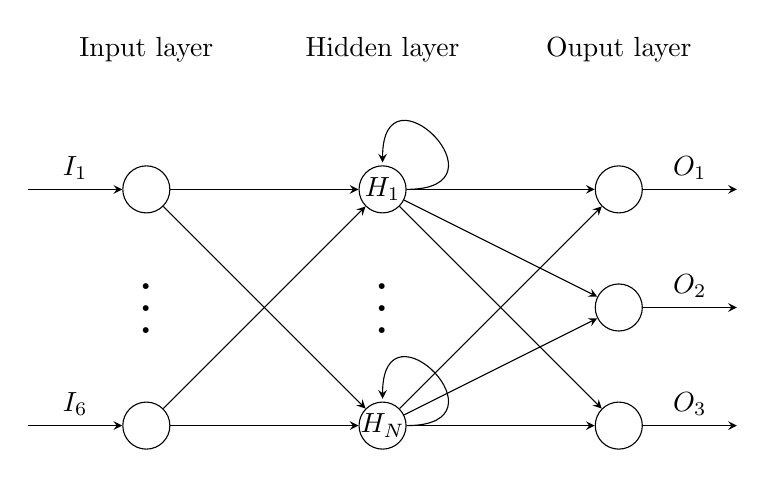
\begin{tikzpicture}[x=1.5cm, y=1.5cm, >=stealth]
        %%%%%%%%%%%%%%%%%%%%%%%%%%%%%%%%%%%%%%%%%%%%
        % Input nodes
        %%%%%%%%%%%%%%%%%%%%%%%%%%%%%%%%%%%%%%%%%%%%
        
        % Drawing
        \foreach \m/\l [count=\y] in {1,missing,2}
            \node [every neuron/.try, neuron \m/.try] (input-\m) at (0,2-\y) {};

        % Labeling
        \foreach \l [count=\i] in {1,6}
            \draw [<-] (input-\i) -- ++(-1,0)
                node [above, midway] {$I_{\l}$};
        
        
        %%%%%%%%%%%%%%%%%%%%%%%%%%%%%%%%%%%%%%%%%%%%
        % Hidden nodes
        %%%%%%%%%%%%%%%%%%%%%%%%%%%%%%%%%%%%%%%%%%%%
        
        % Drawing
        \foreach \m [count=\y] in {1,missing,2}
            \node [every neuron/.try, neuron \m/.try ] (hidden-\m) at (2,2-\y) {};
        
        % Labeling
        \foreach \l [count=\i] in {1,N}
            \node at (hidden-\i) {$H_{\l}$};
        
        \draw[->,shorten >=1pt] (hidden-1) to [out=0,in=90,loop] (hidden-1);
        \draw[->,shorten >=1pt] (hidden-2) to [out=0,in=90,loop] (hidden-2);
        
        %%%%%%%%%%%%%%%%%%%%%%%%%%%%%%%%%%%%%%%%%%%%
        % Output nodes
        %%%%%%%%%%%%%%%%%%%%%%%%%%%%%%%%%%%%%%%%%%%%
        
        % Drawing
        \foreach \m [count=\y] in {1,...,3}
            \node [every neuron/.try, neuron \m/.try ] (output-\m) at (4,2-\y) {};
        
        % Labeling
        \foreach \l [count=\i] in {1,...,3}
            \draw [->] (output-\i) -- ++(1,0)
                node [above, midway] {$O_{\l}$};
        
        
        %%%%%%%%%%%%%%%%%%%%%%%%%%%%%%%%%%%%%%%%%%%%
        % Connecting
        %%%%%%%%%%%%%%%%%%%%%%%%%%%%%%%%%%%%%%%%%%%%
        
        % Input nodes to hidden nodes
        \foreach \i in {1,...,2}
            \foreach \j in {1,...,2}
                \draw [->] (input-\i) -- (hidden-\j);
        
        % Hidden nodes to output nodes
        \foreach \i in {1,...,2}
            \foreach \j in {1,...,3}
                \draw [->] (hidden-\i) -- (output-\j);
        
        
        %%%%%%%%%%%%%%%%%%%%%%%%%%%%%%%%%%%%%%%%%%%%
        % Labeling layers
        %%%%%%%%%%%%%%%%%%%%%%%%%%%%%%%%%%%%%%%%%%%%
        \foreach \l [count=\x from 0] in {Input, Hidden, Ouput}
            \node [align=center, above] at (\x*2,2) {\l\ layer};
    \end{tikzpicture}
    \caption{Previous meetings network structure. N is the number of nodes in the hidden layer.}
    \label{fig:network-previous-meetings-to-result}
\end{figure}

\subsubsection{Input}

The following values are added for each of the previous matches:
\begin{itemize}[noitemsep]
    \item Days since the match, $exp(-\text{days since match} / 730)$. This is added in order to increase the impact of more recent matches.
    \item Goal distribution for the match.
    \item Home team final rating.
    \item Away team final rating.
    \item Final result of the match. $0$ for home victory, $0.5$ for draw, $1$ for away team victory.
\end{itemize}

For each previous match, there are six values. With up to six previous matches, there is a total of $6 * 6 = 36$ features for each match. If two teams have less than six previous matches, a list of six zeros are supplied for each missing match.

For the match between Arsenal and Manchester United May 7, 2017, the input values would be as follows:
\begin{lstlisting}[language=Python]
    [[0.451, 3/3, 0/3, 0.77, 0.63, 0.0]
    [0.293, 1/3, 2/3, 0.65, 0.71, 1.0]
    [0.199, 1/2, 1/2, 0.73, 0.71, 0.5]
    [0.133, 1/2, 1/2, 0.67, 0.67, 0.5]
    [0.071, 1/3, 2/3, 0.67, 0.71, 1.0]
    [0.049, 1/1, 0/1, 0.71, 0.64, 0.0]]
\end{lstlisting}

The hidden layer is a fully connected simple recurrent layer. \cref{fig:network-previous-meetings-to-result} shows the structure of the network. When feeding a match through the network, the previous matches are fed through the hidden layer one by one. The hidden layer output from one match is added to the input for the next.
\subsection{Team characteristics}

This model uses the ideas from \cref{subsec:variables-team-characteristics}. The model also incorporates some of the ideas from \citet{bib:constantinou-fenton-neil-2012}, whereas teams are evaluated anonymously. Teams are represented as the set of their characteristics at match start.

The rationale behind this model is to capture what makes teams win against some opponents, but lose against others. Aside from team strengths and player abilities, what decides a football match? The idea is that the model will capture cases where one team has characteristics that give an advantage over the other team's characteristics. For example if a strength of the home team is "Creating long shot opportunities", whilst a weakness of the away team is "Defending against long shots".

\subsubsection{Input}

Each team is represented as $43$ values in the range $[0, 1]$. Each value corresponds to a team characteristic (see: \cref{subsec:database-overview-team-stats}). Values corresponding to present styles are set to $1$. Strengths and weaknesses are divided by $100$ to fit them into the range $[0, 0.55]$. With $43$ values for each team, that gives a total of $43 * 2 = 86$ features for each match.

For the match between Arsenal and Manchester United May 7, 2017, the input values would be as follows:
\begin{lstlisting}[language=Python]
    [1.0, 1.0, 1.0, 1.0, 0.0, 1.0, 0.0, 0.0, 0.0, 0.0, 0.0, 0.55, 0.55, 0.45, 0.45, 0.0, 0.0, 0.0, 0.25, 0.0, 0.0, 0.0, 0.0, 0.0, 0.0, 0.0, 0.0, 0.0, 0.0, 0.0, 0.15, 0.0, 0.0, 0.0, 0.0, 0.45, 0.0, 0.0, 0.0, 0.45, 1.0, 0.0, 1.0, 1.0, 1.0, 1.0, 0.0, 0.0, 0.0, 1.0, 0.0, 0.0, 1.0, 0.0, 0.25, 0.0, 0.45, 0.0, 0.45, 0.55, 0.45, 0.15, 0.0, 0.0, 0.45, 0.0, 0.0, 0.0, 0.0, 0.0, 0.0, 0.0, 0.0, 0.0, 0.0, 0.0, 0.0, 0.0, 0.55, 0.0, 0.0, 1.0, 0.55, 0.0, 1.0, 1.0]
\end{lstlisting}
The first 43 values are Arsenal characteristics. The last 43 are Manchester United characteristics.
\subsection{Team characteristics and strengths}

This model is an extension of the team characteristics model. In addition to the team characteristics, the model incorporates team strengths. The team strengths are given as final ratings of the starting players after the team's last match, as well as the most recent final rating for the team itself.

\subsubsection{Input}

In addition to the $43$ values for the team characteristics, there are eleven values, one for each player. Lastly, there is an additional value, for the team rating. With $43 + 11 + 1 = 55$ features for each team, there is a total of $55 * 2 = 110$ features for each match.

For the match between Arsenal and Manchester United May 7, 2017, the input values would be as follows:
\begin{lstlisting}[language=Python]
    [0.77, 0.56, 0.67, 0.61, 0.53, 0.65, 0.60, 0.65, 0.63, 0.72, 0.65, 1.0, 1.0, 1.0, 1.0, 0.0, 1.0, 0.0, 0.0, 0.0, 0.0, 0.0, 0.55, 0.55, 0.45, 0.45, 0.0, 0.0, 0.0, 0.25, 0.0, 0.0, 0.0, 0.0, 0.0, 0.0, 0.0, 0.0, 0.0, 0.0, 0.0, 0.15, 0.0, 0.0, 0.0, 0.0, 0.45, 0.0, 0.0, 0.0, 0.45, 1.0, 0.0, 1.0, 0.0, 0.63, 0.70, 0.72, 0.71, 0.68, 0.72, 0.69, 0.75, 0.82, 0.68, 0.78, 0.71, 1.0, 1.0, 1.0, 0.0, 0.0, 0.0, 1.0, 0.0, 0.0, 1.0, 0.0, 0.25, 0.0, 0.45, 0.0, 0.45, 0.55, 0.45, 0.15, 0.0, 0.0, 0.45, 0.0, 0.0, 0.0, 0.0, 0.0, 0.0, 0.0, 0.0, 0.0, 0.0, 0.0, 0.0, 0.0, 0.55, 0.0, 0.0, 1.0, 0.55, 0.0, 1.0, 1.0, 0.0, 0.70]
\end{lstlisting}
\section{Betting simulation}

When evaluating a network in a betting situation, the most promising configuration of the network is used. Ten different prediction model instances are trained, as when measuring prediction accuracy.

To evaluate the profitability of the network, for each network instance, four different betting strategies are used:
\begin{itemize}[noitemsep]
    \item Fixed bet, with $c_{i} = 1$
    \item Fixed return, with $c_{i} = 1 / d_{i}$
    \item Variance adjusted
    \item Kelly ratio, with  $C_{0} = 0.05$
\end{itemize}
Each combination of model instance and strategy is evaluated over the span of two seasons of the English Premier League. The initial bankroll is set to $100$.

For each model instance, the results for each strategy are presented. The development of the \gls{roi} over the span of the season is plotted. The least profitable and most profitable simulations for each strategy are plotted together with the strategy mean.


%========================================================================
%   CHAPTER: EXPERIMENTS
%========================================================================

\chapter{Experiments and results}
\label{chp:experiments-results}
This chapter presents the experiments conducted and the results achieved in this report.

Layer sizes marked with * and ** suffered from overfitting. To overcome the overfitting, dropout was applied. * indicates dropout with $p = 0.1$. ** indicates dropout with $p = 0.2$.

For each network, the share of matches that ended in a home victory is presented. Any accuracy above that level indicates the model has learned something other than to always predict home victory as the most probable outcome.

For each network, strategy, and season, graphs present the development of the \gls{roi} generated by the combination of network and strategy over the given season. The graphs show the least profitable, most profitable, and average \gls{roi} achieved.

For each network and season, graphs showing the connection between predicted probabilities and available odds for every feasible bet were plotted. The lower frontiers of the graphs follow the line $1/P_{i}$, as bets below the line are never deemed feasible. If $d_{i} < 1 / P_{i}$, then $d_{i} * P_{i} < 1$, and the bet will have a negative expected gain.
\section{Benchmark values}

To properly evaluate the networks evaluated in this report, we need some benchmark values. The benchmark values indicate the absolute minimum of what the networks should achieve.

A natural benchmark model is based on the home ground advantage. Of all matches played in the English Premier League August 2009 though May 2015, 46.46\% ended with a home victory, 25.45\% ended draw, and 28.09\% ended with an away victory. \cref{tab:results-benchmark-only-home} shows the \gls{rps} values achieved when predicting all matches in the 2015-2016 and 2016-2016 seasons with the probability distribution [0.4646, 0.2545, 0.2809].
\begin{table}
    \centering
    \begin{tabulary}{\textwidth}{| L || L | L | L |}
        \hline
                        & \multicolumn{3}{ l |}{\textbf{\gls{rps} values}}  \\\hline
        \textbf{Season} & \textbf{Min}  & \textbf{Max}  & \textbf{Mean}     \\\hline
        2015-2016       & 0.141         & 0.355         & 0.227             \\\hline
        2016-2017       & 0.145         & 0.360         & 0.227             \\\hline
    \end{tabulary}
    \caption{RPS values achieved when predicting all matches with the same probability distribution, [0.4646, 0.2545, 0.2809].}
    \label{tab:results-benchmark-only-home} 
\end{table}

Another potential benchmark model is to use the implied probabilities of the bookmakers. The networks are, after all, trying to beat the bookmakers, and not the home ground advantage. \cref{tab:results-benchmark-implied-probabilities} shows the \gls{rps} values achieved when assigning the average implied probabilities of a match as its probability distribution. Using the implied probabilities achieved the best results, and will therefore be used as benchmark values.
\begin{table}
    \centering
    \begin{tabulary}{\textwidth}{| L || L | L | L |}
        \hline
                        & \multicolumn{3}{ l |}{\textbf{\gls{rps} values}}  \\\hline
        \textbf{Season} & \textbf{Min}  & \textbf{Max}  & \textbf{Mean}     \\\hline
        2015-2016       & 0.0333        & 0.683         & 0.210             \\\hline
        2016-2017       & 0.0187        & 0.733         & 0.192             \\\hline
    \end{tabulary}
    \caption{RPS values achieved when predicting all matches with the probability distribution formed by the bookmaker's implied probabilities.}
    \label{tab:results-benchmark-implied-probabilities} 
\end{table}
\section{Player ratings}

\subsection{Network structure}

\cref{tab:results-player-ratings-accuracy} shows the \gls{rps} values and accuracy of the player ratings network. In the evaluation data set, 40.8\% of all matches ended in a home victory.
\begin{table}
    \centering
    \begin{tabulary}{\textwidth}{| L | L || L | L | L || L |}
        \hline
        \multicolumn{2}{| l ||}{\textbf{Hidden layer}}  & \multicolumn{3}{l ||}{\textbf{\gls{rps} values}} & \\\hline
        \textbf{Activation} & \textbf{Size}             & \textbf{Min}  & \textbf{Max}  & \textbf{Mean} & \textbf{Accuracy} \\\hline
        \gls{relu}          & 32                        & 0.0622        & 0.623         & 0.232         & 0.397 \\\hline
        \gls{relu}          & 64                        & 0.0349        & 0.565         & 0.230         & 0.416 \\\hline
        \gls{relu}          & 128                       & 0.0567        & 0.624         & 0.232         & 0.418 \\\hline
        \gls{relu}          & 256                       & 0.0529        & 0.631         & 0.238         & 0.391 \\\hline
        
        \hline
        
        Sigmoid             & 32                        & 0.0377        & 0.640         & 0.233         & 0.413 \\\hline
        Sigmoid             & 64                        & 0.0234        & 0.746         & 0.239         & 0.413 \\\hline
        Sigmoid             & 128                       & 0.0501        & 0.631         & 0.232         & 0.424 \\\hline
        Sigmoid             & 256                       & 0.0484        & 0.637         & 0.236         & 0.410 \\\hline
        Sigmoid             & 512*                      & 0.0265        & 0.711         & 0.241         & 0.408 \\\hline
        
        \hline
        
        \Gls{tanh}          & 32                        & 0.0728        & 0.569         & 0.234         & 0.386 \\\hline
        \Gls{tanh}          & 64                        & 0.0368        & 0.732         & 0.239         & 0.399 \\\hline
        \Gls{tanh}          & 128                       & 0.0349        & 0.647         & 0.234         & 0.402 \\\hline
        \rowcolor{correct}
        \Gls{tanh}          & 256*                      & 0.0674        & 0.554         & 0.228         & 0.426 \\\hline
        \Gls{tanh}          & 512*                      & 0.0467        & 0.652         & 0.233         & 0.413 \\\hline
    \end{tabulary}
    \caption{Prediction accuracy of the player ratings network, with different hidden layer configurations. The row colored green shows the configuration with most promising results.}
    \label{tab:results-player-ratings-accuracy} 
\end{table}

Using a hidden layer with 256 nodes activated by the \gls{tanh} function yielded the most promising results, and will therefore be used when evaluating the profitability of the network. \cref{tab:results-player-ratings-accuracy-2016-2017} shows the \gls{rps} values and prediction accuracy when evaluating the same configuration over the 2016-2017 season. Unfortunately, the network did not perform better than the benchmark model for any of the seasons.
\begin{table}
    \centering
    \begin{tabulary}{\textwidth}{| L | L | L || L |}
        \hline
        \multicolumn{3}{| l ||}{\textbf{\gls{rps} values}}  &                   \\\hline
        \textbf{Min}    & \textbf{Max}  & \textbf{Mean}     & \textbf{Accuracy} \\\hline
        0.0390          & 0.721         & 0.223             & 0.507             \\\hline
    \end{tabulary}
    \caption{Prediction accuracy of the player ratings network for the 2016-2017 season of the English Premier League, using the most promising hidden layer configuration.}
    \label{tab:results-player-ratings-accuracy-2016-2017} 
\end{table}

\subsection{Betting results}

\subsubsection{English Premier League 2015-2016}

\cref{fig:results-player-ratings-2015-2016-fixed-bet,fig:results-player-ratings-2015-2016-fixed-return,fig:results-player-ratings-2015-2016-kelly-ratio,fig:results-player-ratings-2015-2016-variance-adjusted} show the development of the \gls{roi} generated by the player ratings network over the English Premier League season 2015-2016.
\begin{figure}
    \centering
    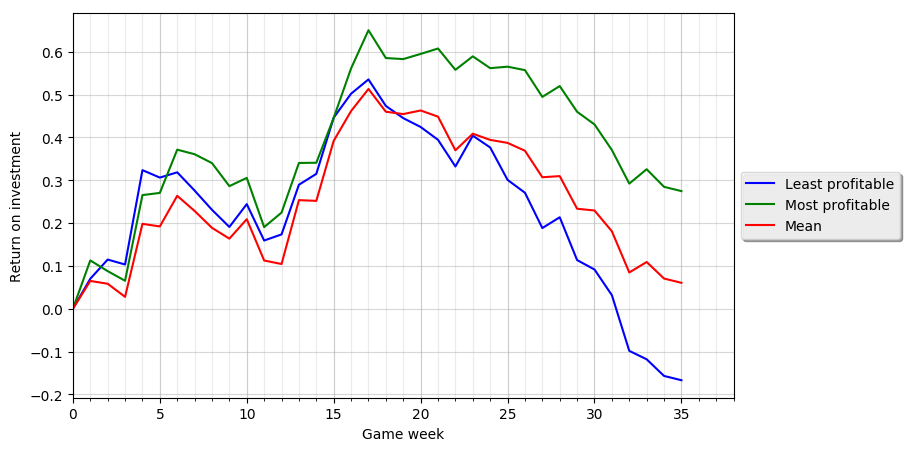
\includegraphics[width=\textwidth]{results/player-ratings/2015-2016/fixed-bet-10.png}
    \caption{\gls{roi} over the span of the English Premier League season 2015-2016 using the player ratings network and the fixed bet strategy.}
    \label{fig:results-player-ratings-2015-2016-fixed-bet}
\end{figure}
\begin{figure}
    \centering
    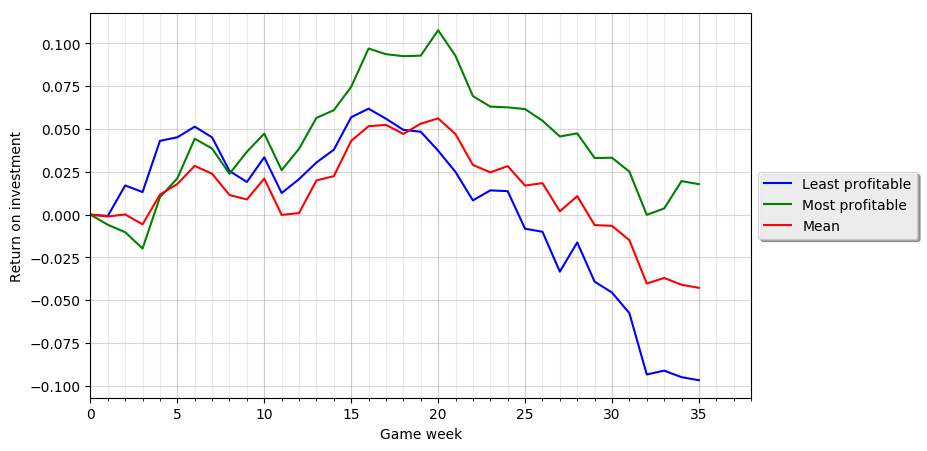
\includegraphics[width=\textwidth]{results/player-ratings/2015-2016/fixed-return-10.png}
    \caption{\gls{roi} over the span of the English Premier League season 2015-2016 using the player ratings network and the fixed return strategy.}
    \label{fig:results-player-ratings-2015-2016-fixed-return}
\end{figure}
\begin{figure}
    \centering
    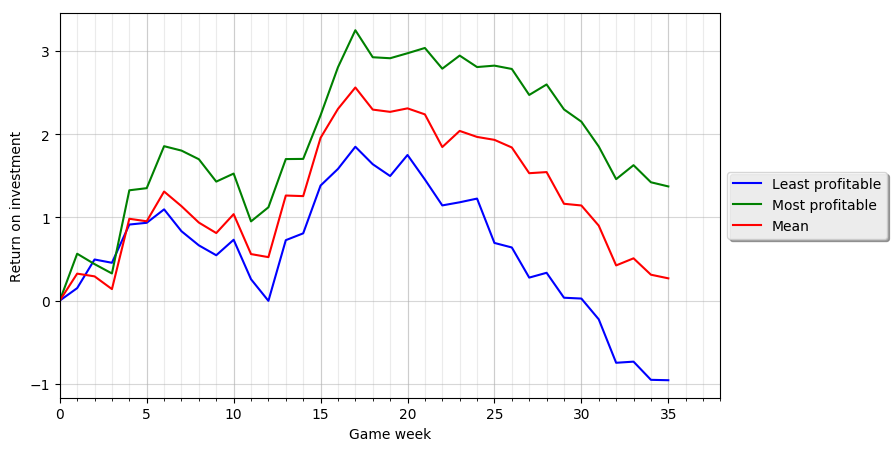
\includegraphics[width=\textwidth]{results/player-ratings/2015-2016/kelly-ratio-10.png}
    \caption{\gls{roi} over the span of the English Premier League season 2015-2016 using the player ratings network and the Kelly ratio strategy.}
    \label{fig:results-player-ratings-2015-2016-kelly-ratio}
\end{figure}
\begin{figure}
    \centering
    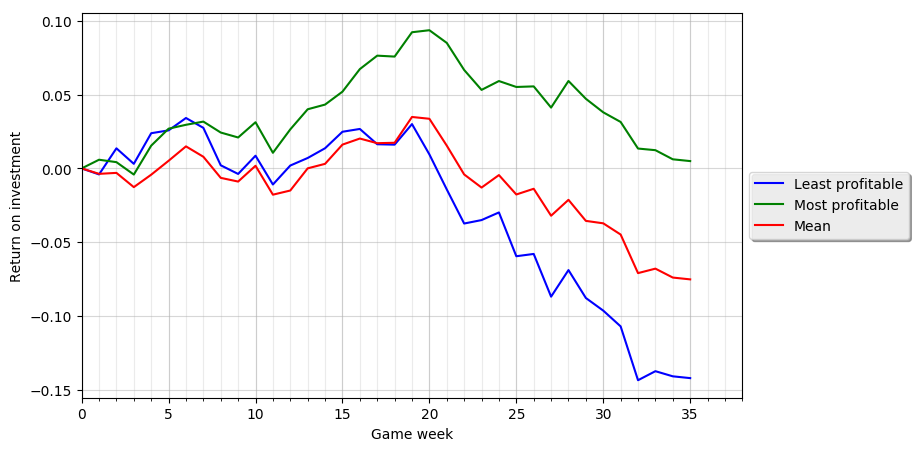
\includegraphics[width=\textwidth]{results/player-ratings/2015-2016/variance-adjusted-10.png}
    \caption{\gls{roi} over the span of the English Premier League season 2015-2016 using the player ratings network and the variance adjusted strategy.}
    \label{fig:results-player-ratings-2015-2016-variance-adjusted}
\end{figure}

\cref{tab:fig:results-player-ratings-2015-2016-roi} shows a summary of the \gls{roi} values achieved by the different strategies when used by the player ratings network. The table shows the final \gls{roi} for the least profitable and most profitable simulations, together with the average final \gls{roi}.
\begin{table}
    \centering
    \begin{tabulary}{\textwidth}{| L || L | L | L |}
        \hline
                            & \multicolumn{3}{l |}{\textbf{Final \gls{roi}}} \\\hline
        \textbf{Strategy}   & \textbf{Min}  & \textbf{Max}  & \textbf{Mean} \\\hline
        Fixed bet           & -0.16         & 0.28          & 0.068 \\\hline
        Fixed return        & -0.098        & 0.022         & -0.040 \\\hline
        Kelly ratio         & -0.99         & 1.4           & \cellcolor{correct} 0.25 \\\hline
        Variance adjusted   & -0.14         & 0.010         & -0.073 \\\hline
    \end{tabulary}
    \caption{Final \gls{roi} values for the four strategies when using the player ratings network during the 2015-2016 season of the English Premier League. The green colored cell was the most profitable strategy (on average).}
    \label{tab:fig:results-player-ratings-2015-2016-roi}
\end{table}
        
\cref{fig:results-player-ratings-2015-2016-odds-prob} shows the bets placed during the 2015-2016 season of the English Premier League. The probabilities are generated by a random instance of the player ratings network.
\begin{figure}
    \centering
    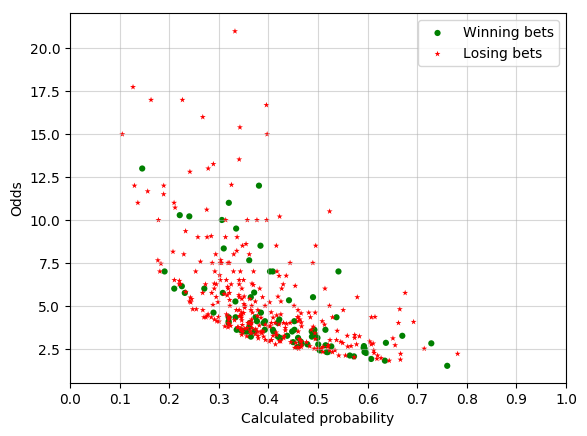
\includegraphics[width=\textwidth]{results/player-ratings/2015-2016/odds-prob.png}
    \caption{Offered odds and predicted probabilities for the bets placed during the 2015-2016 season of the English Premier League. The probabilities are generated by the player ratings network.}
    \label{fig:results-player-ratings-2015-2016-odds-prob}
\end{figure}


\subsubsection{English Premier League 2016-2017}

\cref{fig:results-player-ratings-2016-2017-fixed-bet,fig:results-player-ratings-2016-2017-fixed-return,fig:results-player-ratings-2016-2017-kelly-ratio,fig:results-player-ratings-2016-2017-variance-adjusted} show the development of the \gls{roi} generated by the player ratings network over the English Premier League season 2016-2017.
\begin{figure}
    \centering
    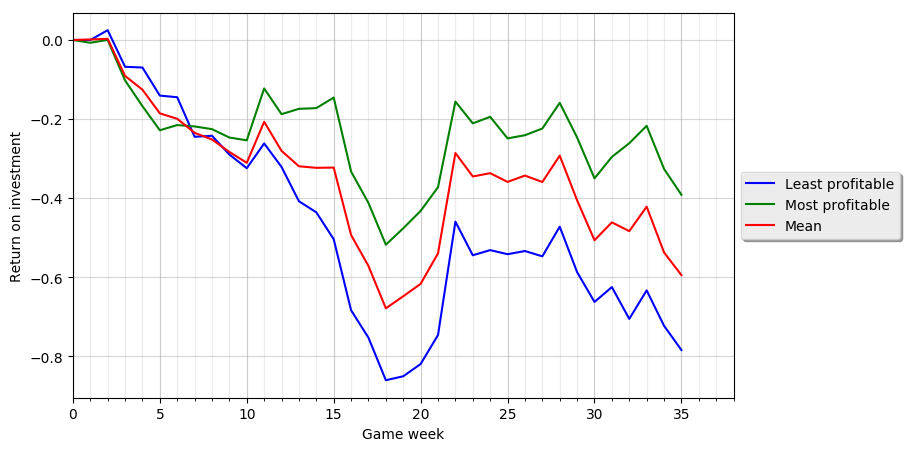
\includegraphics[width=\textwidth]{results/player-ratings/2016-2017/fixed-bet-10.png}
    \caption{\gls{roi} over the span of the English Premier League season 2016-2017 using the player ratings network and the fixed bet strategy.}
    \label{fig:results-player-ratings-2016-2017-fixed-bet}
\end{figure}
\begin{figure}
    \centering
    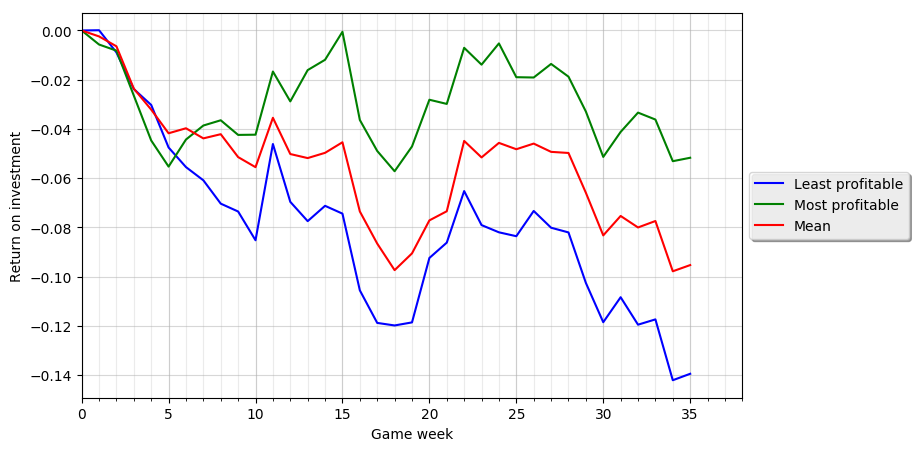
\includegraphics[width=\textwidth]{results/player-ratings/2016-2017/fixed-return-10.png}
    \caption{\gls{roi} over the span of the English Premier League season 2016-2017 using the player ratings network and the fixed return strategy.}
    \label{fig:results-player-ratings-2016-2017-fixed-return}
\end{figure}
\begin{figure}
    \centering
    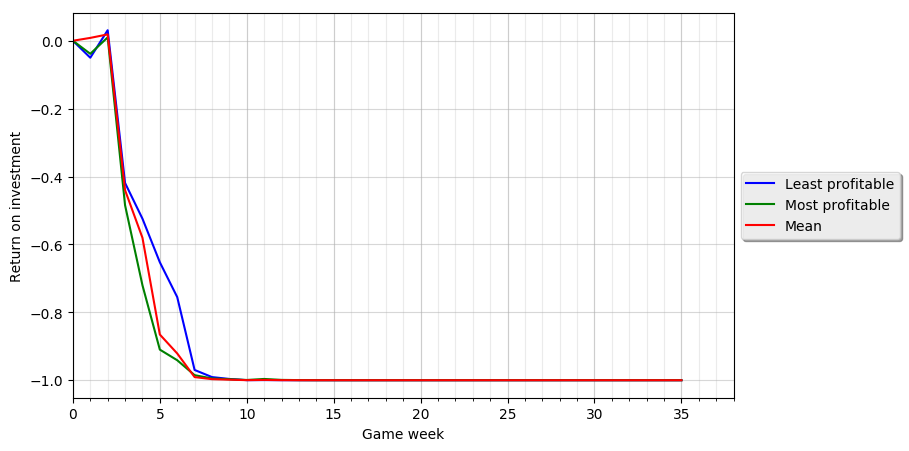
\includegraphics[width=\textwidth]{results/player-ratings/2016-2017/kelly-ratio-10.png}
    \caption{\gls{roi} over the span of the English Premier League season 2016-2017 using the player ratings network and the Kelly ratio strategy.}
    \label{fig:results-player-ratings-2016-2017-kelly-ratio}
\end{figure}
\begin{figure}
    \centering
    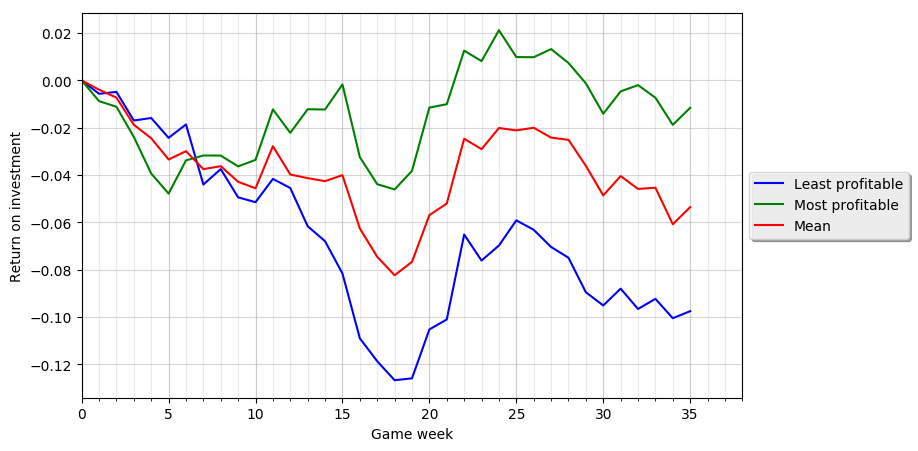
\includegraphics[width=\textwidth]{results/player-ratings/2016-2017/variance-adjusted-10.png}
    \caption{\gls{roi} over the span of the English Premier League season 2016-2017 using the player ratings network and the variance adjusted strategy.}
    \label{fig:results-player-ratings-2016-2017-variance-adjusted}
\end{figure}

\cref{tab:fig:results-player-ratings-2016-2017-roi} shows a summary of the \gls{roi} values achieved by the different strategies when used by the player ratings network. The table shows the final \gls{roi} for the least profitable and most profitable simulations, together with the average final \gls{roi}.
\begin{table}
    \centering
    \begin{tabulary}{\textwidth}{| L || L | L | L |}
        \hline
                            & \multicolumn{3}{l |}{\textbf{Final \gls{roi}}} \\\hline
        \textbf{Strategy}   & \textbf{Min}  & \textbf{Max}  & \textbf{Mean} \\\hline
        Fixed bet           & -0.78         & -0.38         & -0.59 \\\hline
        Fixed return        & -0.14         & -0.050        & -0.095 \\\hline
        Kelly ratio         & -1.0          & -1.0          & -1.0 \\\hline
        Variance adjusted   & -0.098        & -0.013        & \cellcolor{correct} -0.053 \\\hline
    \end{tabulary}
    \caption{Final \gls{roi} values for the four strategies when using the player ratings network during the 2016-2017 season of the English Premier League. The green colored cell was the most profitable strategy (on average).}
    \label{tab:fig:results-player-ratings-2016-2017-roi}
\end{table}

\cref{fig:results-player-ratings-2016-2017-odds-prob} shows the bets placed during the 2016-2017 season of the English Premier League. The probabilities are generated by a random instance of the player ratings network.
\begin{figure}
    \centering
    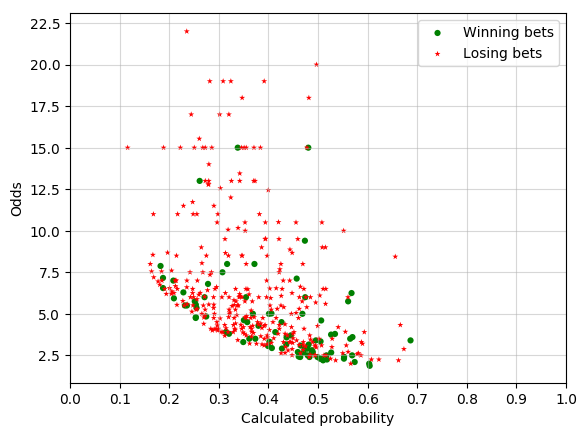
\includegraphics[width=\textwidth]{results/player-ratings/2016-2017/odds-prob.png}
    \caption{Offered odds and predicted probabilities for the bets placed during the 2016-2017 season of the English Premier League. The probabilities are generated by the player ratings network.}
    \label{fig:results-player-ratings-2016-2017-odds-prob}
\end{figure}


\subsubsection{Summary}

The network did not achieve consistent good results. The first season, the Kelly ratio strategy was the only strategy to generate a profit. The second season, however, the strategy went bankrupt.

\cref{fig:results-player-ratings-2015-2016-odds-prob,fig:results-player-ratings-2016-2017-odds-prob} show the connection between odds and probabilities predicted by the player ratings network. The player ratings network tend to overestimate the probability of too many high-odds outcomes. A great portion of the bets in the lower half of the horizontal axis are overestimated. The overestimates contribute a lot to the lack of profitability of the network. Over the two seasons, the prediction models won approximately 20.4\% of all bets placed, with an average odds of 4.34.

\section{Head to head}

\subsection{Network structure}

\cref{tab:results-head-to-head-accuracy} shows the \gls{rps} values and accuracy of the head to head network. In the evaluation data set, 38.1\% of all matches ended in a home victory.
\begin{table}
    \centering
    \begin{tabulary}{\textwidth}{| L | L || L | L | L || L |}
        \hline
        \multicolumn{2}{| l ||}{\textbf{Hidden layer}}  & \multicolumn{3}{l ||}{\textbf{\gls{rps} values}} & \\\hline
        \textbf{Activation} & \textbf{Size}             & \textbf{Min}  & \textbf{Max}  & \textbf{Mean} & \textbf{Accuracy} \\\hline
        \gls{relu}          & 16                        & 0.127         & 0.479         & 0.300         & 0.387 \\\hline
        \gls{relu}          & 32                        & 0.0733        & 0.571         & 0.234         & 0.391 \\\hline
        \gls{relu}          & 64                        & 0.0889        & 0.548         & 0.232         & 0.397 \\\hline
        \gls{relu}          & 128                       & 0.0692        & 0.586         & 0.238         & 0.387 \\\hline
        
        \hline
        
        Sigmoid             & 16                        & 0.0823        & 0.553         & 0.236         & 0.394 \\\hline
        \rowcolor{correct}
        Sigmoid             & 32                        & 0.111         & 0.468         & 0.228         & 0.401 \\\hline
        Sigmoid             & 64                        & 0.081         & 0.557         & 0.232         & 0.381 \\\hline
        
        \hline
        
        \Gls{tanh}          & 16                        & 0.0904        & 0.537         & 0.232         & 0.397 \\\hline
        \Gls{tanh}          & 32                        & 0.0883        & 0.537         & 0.231         & 0.384 \\\hline
        \Gls{tanh}          & 64                        & 0.0959        & 0.523         & 0.230         & 0.384 \\\hline
    \end{tabulary}
    \caption{Accuracy of the head to head network, with different hidden layer configurations. The row colored green shows the configuration with most promising results.}
    \label{tab:results-head-to-head-accuracy} 
\end{table}

Using a hidden layer with 32 nodes activated by the sigmoid function yielded the most promising results, and will therefore be used when evaluating the profitability of the network. \cref{tab:results-head-to-head-accuracy-2016-2017} shows the \gls{rps} values and prediction accuracy when evaluating the same configuration over the 2016-2017 season. Unfortunately, the network did not perform better than the benchmark model for any of the seasons.
\begin{table}
    \centering
    \begin{tabulary}{\textwidth}{| L | L | L || L |}
        \hline
        \multicolumn{3}{| l ||}{\textbf{\gls{rps} values}}  &                   \\\hline
        \textbf{Min}    & \textbf{Max}  & \textbf{Mean}     & \textbf{Accuracy} \\\hline
        0.0933          & 0.727         & 0.220             & 0.497             \\\hline
    \end{tabulary}
    \caption{Prediction accuracy of the head to head network for the 2016-2017 season of the English Premier League, using the most promising hidden layer configuration.}
    \label{tab:results-head-to-head-accuracy-2016-2017} 
\end{table}


\subsection{Betting results}

\subsubsection{English Premier League 2015-2016}

\cref{fig:results-head-to-head-2015-2016-fixed-bet,fig:results-head-to-head-2015-2016-fixed-return,fig:results-head-to-head-2015-2016-kelly-ratio,fig:results-head-to-head-2015-2016-variance-adjusted} show the development of the \gls{roi} generated by the head to head network over the English Premier League season 2015-2016.
\begin{figure}
    \centering
    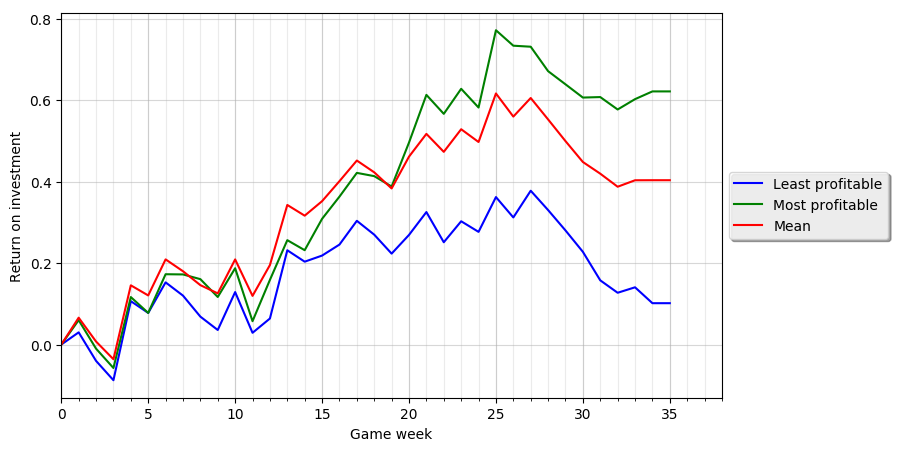
\includegraphics[width=\textwidth]{results/head-to-head/2015-2016/fixed-bet-10.png}
    \caption{\gls{roi} over the span of the English Premier League season 2015-2016 using the head to head network and the fixed bet strategy.}
    \label{fig:results-head-to-head-2015-2016-fixed-bet}
\end{figure}
\begin{figure}
    \centering
    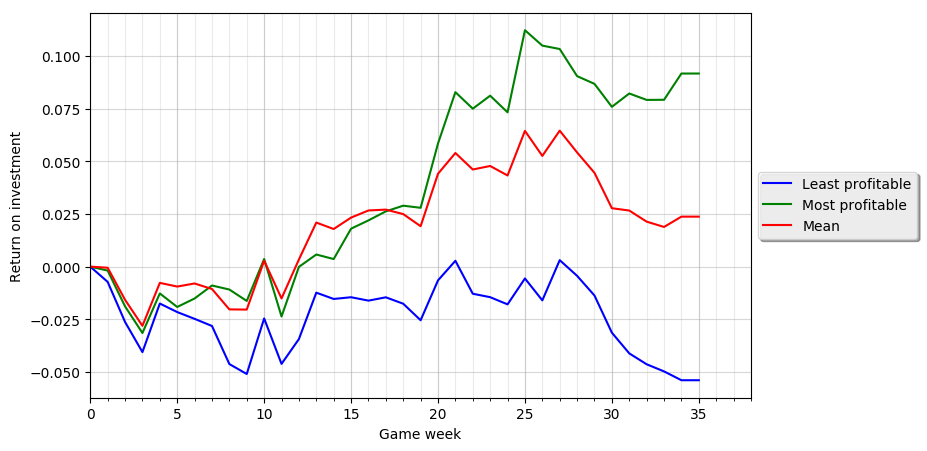
\includegraphics[width=\textwidth]{results/head-to-head/2015-2016/fixed-return-10.png}
    \caption{\gls{roi} over the span of the English Premier League season 2015-2016 using the head to head network and the fixed return strategy.}
    \label{fig:results-head-to-head-2015-2016-fixed-return}
\end{figure}
\begin{figure}
    \centering
    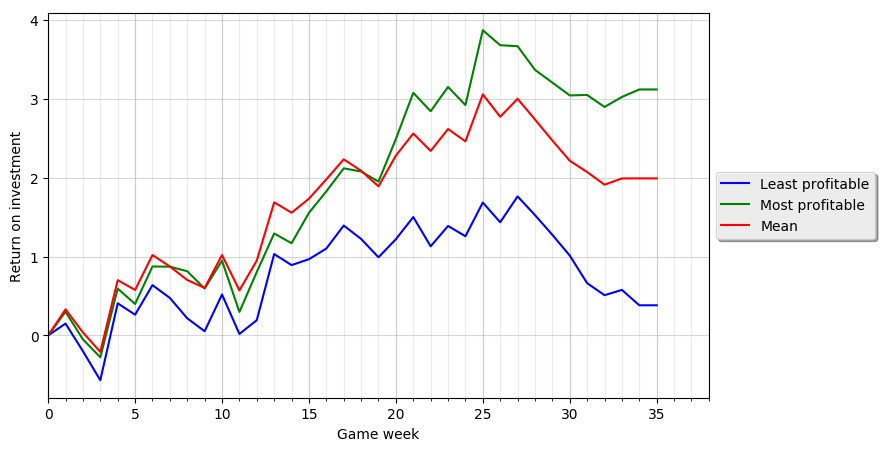
\includegraphics[width=\textwidth]{results/head-to-head/2015-2016/kelly-ratio-10.png}
    \caption{\gls{roi} over the span of the English Premier League season 2015-2016 using the head to head network and the Kelly ratio strategy.}
    \label{fig:results-head-to-head-2015-2016-kelly-ratio}
\end{figure}
\begin{figure}
    \centering
    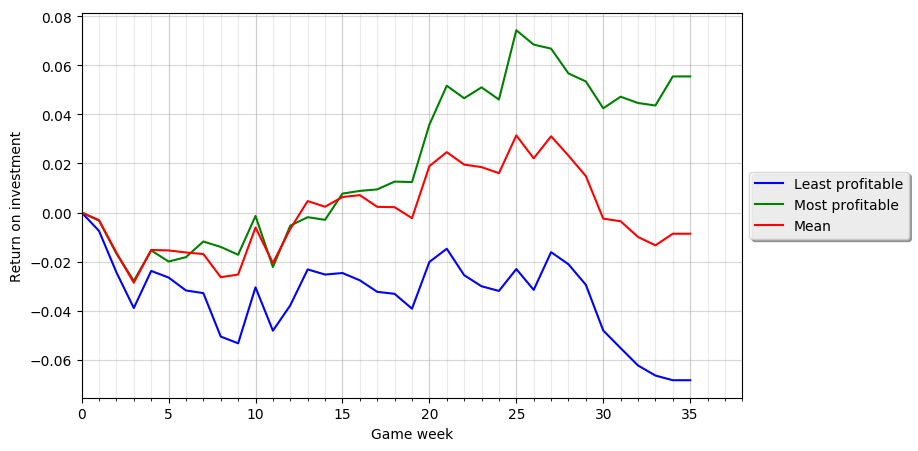
\includegraphics[width=\textwidth]{results/head-to-head/2015-2016/variance-adjusted-10.png}
    \caption{\gls{roi} over the span of the English Premier League season 2015-2016 using the head to head network and the variance adjusted strategy.}
    \label{fig:results-head-to-head-2015-2016-variance-adjusted}
\end{figure}

\cref{tab:fig:results-head-to-head-2015-2016-roi} shows a summary of the \gls{roi} values achieved by the different strategies when used by the head to head network. The table shows the final \gls{roi} for the least profitable and most profitable simulations, together with the average final \gls{roi}.
\begin{table}
    \centering
    \begin{tabulary}{\textwidth}{| L || L | L | L |}
        \hline
                            & \multicolumn{3}{l |}{\textbf{Final \gls{roi}}} \\\hline
        \textbf{Strategy}   & \textbf{Min}  & \textbf{Max}  & \textbf{Mean} \\\hline
        Fixed bet           & 0.16          & 0.61          & 0.40 \\\hline
        Fixed return        & -0.053        & 0.092         & 0.025 \\\hline
        Kelly ratio         & 0.44          & 3.1           & \cellcolor{correct} 2.0 \\\hline
        Variance adjusted   & -0.070        & 0.057         & -0.0080 \\\hline
    \end{tabulary}
    \caption{Final \gls{roi} values for the four strategies when using the head to head network during the 2015-2016 season of the English Premier League. The green colored cell was the most profitable strategy (on average).}
    \label{tab:fig:results-head-to-head-2015-2016-roi}
\end{table}
  
\cref{fig:results-head-to-head-2015-2016-odds-prob} shows the bets placed during the 2015-2016 season of the English Premier League. The probabilities are generated by a random instance of the head to head network.
\begin{figure}
    \centering
    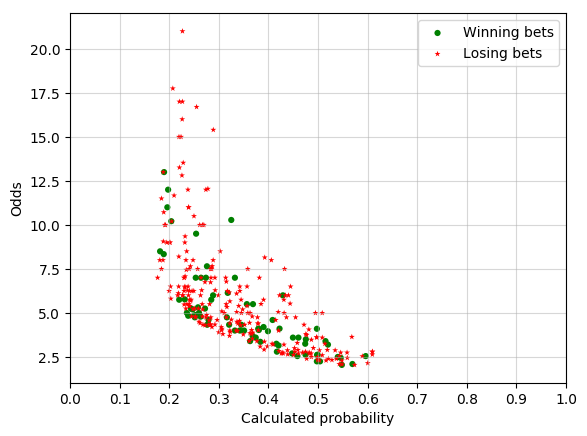
\includegraphics[width=\textwidth]{results/head-to-head/2015-2016/odds-prob.png}
    \caption{Offered odds and predicted probabilities for the bets placed during the 2015-2016 season of the English Premier League. The probabilities are generated by the head to head network.}
    \label{fig:results-head-to-head-2015-2016-odds-prob}
\end{figure}
      

\subsubsection{English Premier League 2016-2017}

\cref{fig:results-head-to-head-2016-2017-fixed-bet,fig:results-head-to-head-2016-2017-fixed-return,fig:results-head-to-head-2016-2017-kelly-ratio,fig:results-head-to-head-2016-2017-variance-adjusted} show the development of the \gls{roi} generated by the head to head network over the English Premier League season 2016-2017.
\begin{figure}
    \centering
    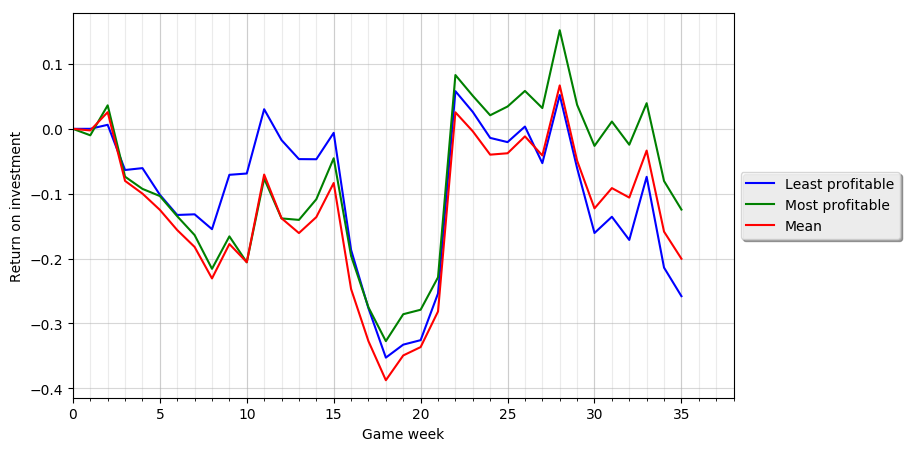
\includegraphics[width=\textwidth]{results/head-to-head/2016-2017/fixed-bet-10.png}
    \caption{\gls{roi} over the span of the English Premier League season 2016-2017 using the head to head network and the fixed bet strategy.}
    \label{fig:results-head-to-head-2016-2017-fixed-bet}
\end{figure}
\begin{figure}
    \centering
    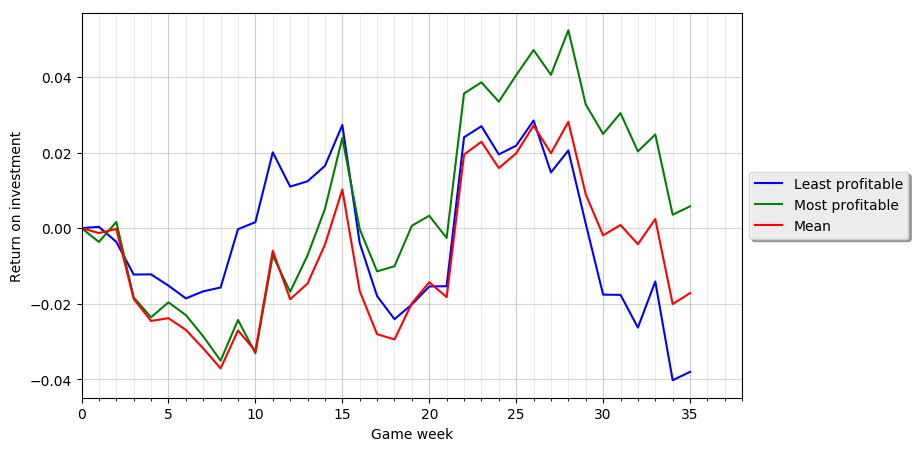
\includegraphics[width=\textwidth]{results/head-to-head/2016-2017/fixed-return-10.png}
    \caption{\gls{roi} over the span of the English Premier League season 2016-2017 using the head to head network and the fixed return strategy.}
    \label{fig:results-head-to-head-2016-2017-fixed-return}
\end{figure}
\begin{figure}
    \centering
    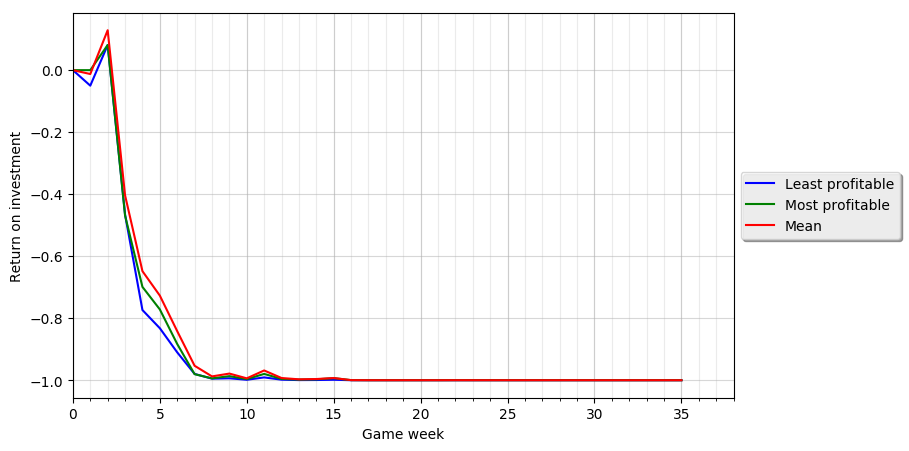
\includegraphics[width=\textwidth]{results/head-to-head/2016-2017/kelly-ratio-10.png}
    \caption{\gls{roi} over the span of the English Premier League season 2016-2017 using the head to head network and the Kelly ratio strategy.}
    \label{fig:results-head-to-head-2016-2017-kelly-ratio}
\end{figure}
\begin{figure}
    \centering
    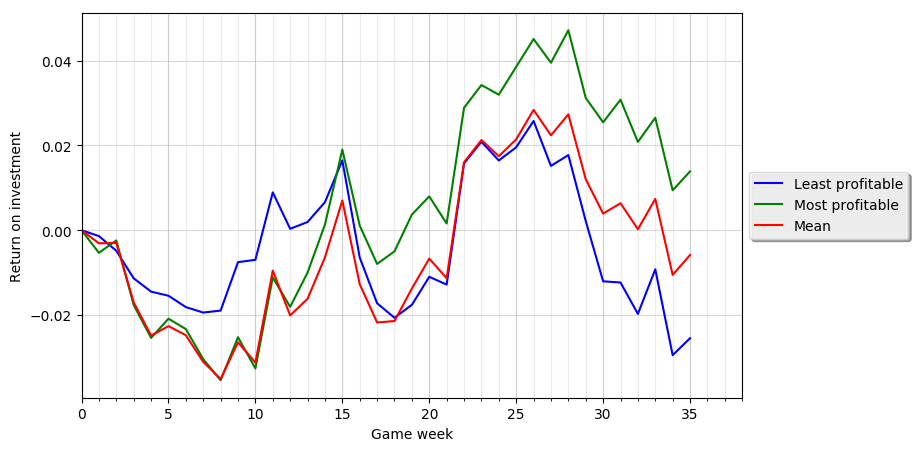
\includegraphics[width=\textwidth]{results/head-to-head/2016-2017/variance-adjusted-10.png}
    \caption{\gls{roi} over the span of the English Premier League season 2016-2017 using the head to head network and the variance adjusted strategy.}
    \label{fig:results-head-to-head-2016-2017-variance-adjusted}
\end{figure}

\cref{tab:fig:results-head-to-head-2016-2017-roi} shows a summary of the \gls{roi} values achieved by the different strategies when used by the head to head network. The table shows the final \gls{roi} for the least profitable and most profitable simulations, together with the average final \gls{roi}.
\begin{table}
    \centering
    \begin{tabulary}{\textwidth}{| L || L | L | L |}
        \hline
                            & \multicolumn{3}{l |}{\textbf{Final \gls{roi}}} \\\hline
        \textbf{Strategy}   & \textbf{Min}  & \textbf{Max}  & \textbf{Mean} \\\hline
        Fixed bet           & -0.25         & -0.12         & -0.20 \\\hline
        Fixed return        & -0.038        & 0.07          & -0.018 \\\hline
        Kelly ratio         & -1.0          & -1.0          & -1.0 \\\hline
        Variance adjusted   & -0.024        & 0.014         & \cellcolor{correct} -0.0060 \\\hline
    \end{tabulary}
    \caption{Final \gls{roi} values for the four strategies when using the head to head network during the 2016-2017 season of the English Premier League. The green colored cell was the most profitable strategy (on average).}
    \label{tab:fig:results-head-to-head-2016-2017-roi}
\end{table}

\cref{fig:results-head-to-head-2016-2017-odds-prob} shows the bets placed during the 2016-2017 season of the English Premier League. The probabilities are generated by a random instance of the head to head network.
\begin{figure}
    \centering
    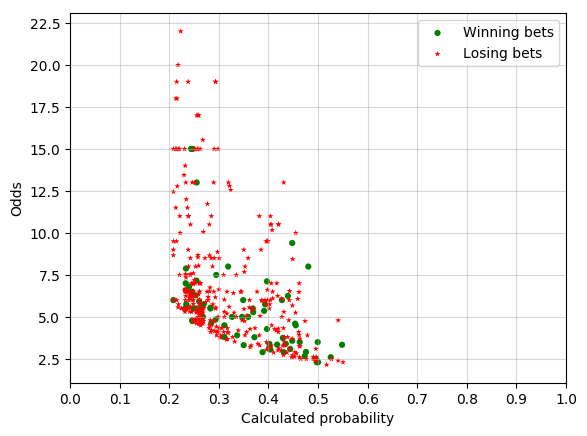
\includegraphics[width=\textwidth]{results/head-to-head/2016-2017/odds-prob.png}
    \caption{Offered odds and predicted probabilities for the bets placed during the 2016-2017 season of the English Premier League. The probabilities are generated by the head to head network.}
    \label{fig:results-head-to-head-2016-2017-odds-prob}
\end{figure}


\subsubsection{Summary}

The network did not achieve consistent good results. The first season, the fixed bet and Kelly ratio strategies performed well, gaining profits for all instances. The second season, however, the same strategies achieved \glspl{roi} of -0.25 and -1.0, respectively.

\cref{fig:results-head-to-head-2015-2016-odds-prob,fig:results-head-to-head-2016-2017-odds-prob} show the connection between odds and probabilities predicted by the head to head network. The head to head network struggles with sparse predictions. This is likely due to how rapidly teams change in football. Between each season, and in January, teams have the opportunity to buy and sell players. A team being relegated from the English Premier League might be forced to sell their best players, reducing their strengths. Other teams receive a lot of money from their owners, making them able to improve their squad greatly between two seasons. This makes it difficult to predict the results of a match based on the previous meetings between the two teams. The training procedure therefore approximates the outcome distribution in the training data set. Over the two seasons, the prediction models won approximately 19.2\% of all bets placed, with an average odds of 4.89.
\section{Previous meetings}

\subsection{Network structure}

\cref{tab:results-previous-meetings-accuracy} shows the \gls{rps} values and accuracy of the previous meetings network. In the evaluation data set, 38.1\% of all matches ended in a home victory.
\begin{table}
    \centering
    \begin{tabulary}{\textwidth}{| L | L || L | L | L || L |}
        \hline
        \multicolumn{2}{| l ||}{\textbf{Hidden layer}}  & \multicolumn{3}{l ||}{\textbf{\gls{rps} values}} & \\\hline
        \textbf{Activation} & \textbf{Size}             & \textbf{Min}  & \textbf{Max}  & \textbf{Mean} & \textbf{Accuracy} \\\hline
        \gls{relu}          & 32                        & 0.0525        & 0.585         & 0.235         & 0.374 \\\hline
        \gls{relu}          & 64                        & 0.0425        & 0.616         & 0.236         & 0.381 \\\hline
        \gls{relu}          & 128                       & 0.0505        & 0.616         & 0.242         & 0.358 \\\hline
        
        \hline
        
        Sigmoid             & 32                        & 0.125         & 0.457         & 0.228         & 0.374 \\\hline
        Sigmoid             & 64                        & 0.138         & 0.436         & 0.236         & 0.381 \\\hline
        Sigmoid             & 128                       & 0.133         & 0.371         & 0.228         & 0.381 \\\hline
        Sigmoid             & 256                       & 0.112         & 0.484         & 0.230         & 0.381 \\\hline
        
        \hline
        
        \Gls{tanh}          & 32                        & 0.0342        & 0.650         & 0.249         & 0.354 \\\hline
        \Gls{tanh}          & 64                        & 0.0573        & 0.619         & 0.237         & 0.361 \\\hline
        \rowcolor{correct}
        \Gls{tanh}          & 128                       & 0.0352        & 0.646         & 0.236         & 0.394 \\\hline
        \Gls{tanh}          & 256                       & 0.0340        & 0.671         & 0.248         & 0.381 \\\hline
    \end{tabulary}
    \caption{Accuracy of the previous meetings network, with different hidden layer configurations. The row colored green shows the configuration with most promising results.}
    \label{tab:results-previous-meetings-accuracy} 
\end{table}

Using a hidden layer with 128 nodes activated by the \gls{tanh} function yielded the most promising results, and will therefore be used when evaluating the profitability of the network. \cref{tab:results-previous-meetings-accuracy-2016-2017} shows the \gls{rps} values and prediction accuracy when evaluating the same configuration over the 2016-2017 season. Unfortunately, the network did not perform better than the benchmark model for any of the seasons.
\begin{table}
    \centering
    \begin{tabulary}{\textwidth}{| L | L | L || L |}
        \hline
        \multicolumn{3}{| l ||}{\textbf{\gls{rps} values}}  &                   \\\hline
        \textbf{Min}    & \textbf{Max}  & \textbf{Mean}     & \textbf{Accuracy} \\\hline
        0.0807          & 0.657         & 0.217             & 0.503             \\\hline
    \end{tabulary}
    \caption{Prediction accuracy of the previous meetings network for the 2016-2017 season of the English Premier League, using the most promising hidden layer configuration.}
    \label{tab:results-previous-meetings-accuracy-2016-2017} 
\end{table}


\subsection{Betting results}

\subsubsection{English Premier League 2015-2016}

\cref{fig:results-previous-meetings-2015-2016-fixed-bet,fig:results-previous-meetings-2015-2016-fixed-return,fig:results-previous-meetings-2015-2016-kelly-ratio,fig:results-previous-meetings-2015-2016-variance-adjusted} show the development of the \gls{roi} generated by the previous meetings network over the English Premier League season 2015-2016.
\begin{figure}
    \centering
    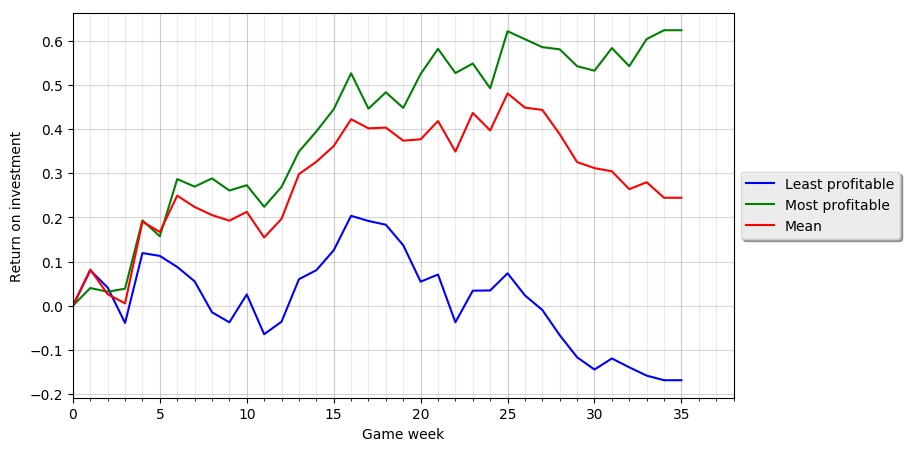
\includegraphics[width=\textwidth]{results/previous-meetings/2015-2016/fixed-bet-10.png}
    \caption{\gls{roi} over the span of the English Premier League season 2015-2016 using the previous meetings network and the fixed bet strategy.}
    \label{fig:results-previous-meetings-2015-2016-fixed-bet}
\end{figure}
\begin{figure}
    \centering
    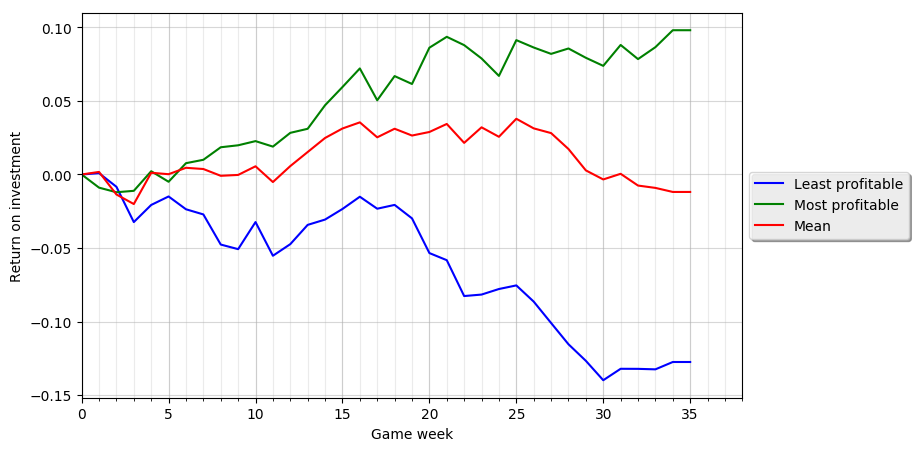
\includegraphics[width=\textwidth]{results/previous-meetings/2015-2016/fixed-return-10.png}
    \caption{\gls{roi} over the span of the English Premier League season 2015-2016 using the previous meetings network and the fixed return strategy.}
    \label{fig:results-previous-meetings-2015-2016-fixed-return}
\end{figure}
\begin{figure}
    \centering
    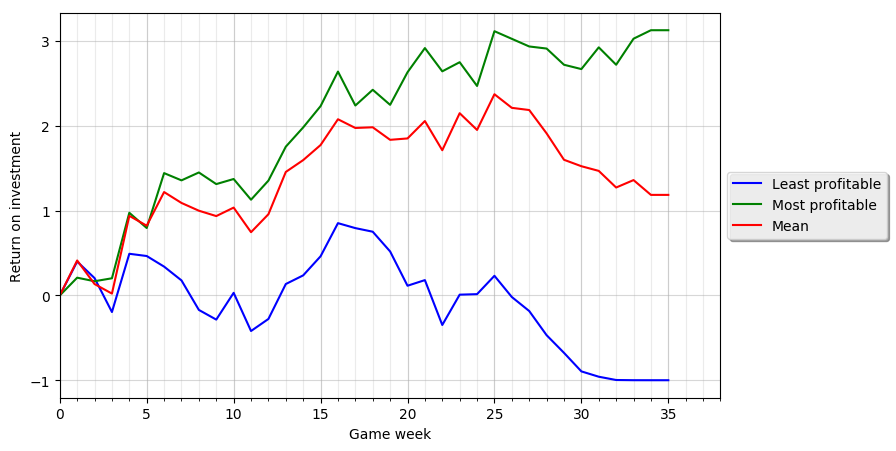
\includegraphics[width=\textwidth]{results/previous-meetings/2015-2016/kelly-ratio-10.png}
    \caption{\gls{roi} over the span of the English Premier League season 2015-2016 using the previous meetings network and the Kelly ratio strategy.}
    \label{fig:results-previous-meetings-2015-2016-kelly-ratio}
\end{figure}
\begin{figure}
    \centering
    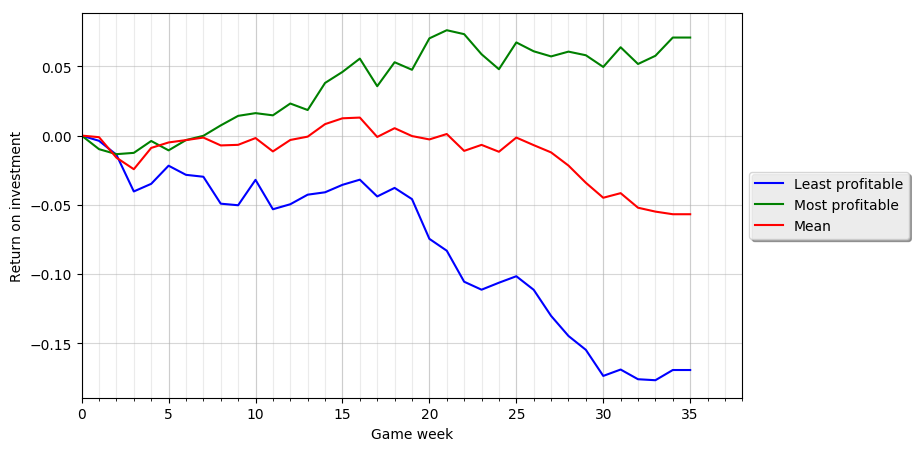
\includegraphics[width=\textwidth]{results/previous-meetings/2015-2016/variance-adjusted-10.png}
    \caption{\gls{roi} over the span of the English Premier League season 2015-2016 using the previous meetings network and the variance adjusted strategy.}
    \label{fig:results-previous-meetings-2015-2016-variance-adjusted}
\end{figure}

\cref{tab:fig:results-previous-meetings-2015-2016-roi} shows a summary of the \gls{roi} values achieved by the different strategies when used by the previous meetings network. The table shows the final \gls{roi} for the least profitable and most profitable simulations, together with the average final \gls{roi}.
\begin{table}
    \centering
    \begin{tabulary}{\textwidth}{| L || L | L | L |}
        \hline
                            & \multicolumn{3}{l |}{\textbf{Final \gls{roi}}} \\\hline
        \textbf{Strategy}   & \textbf{Min}  & \textbf{Max}  & \textbf{Mean} \\\hline
        Fixed bet           & -0.17         & 0.62          & 0.25 \\\hline
        Fixed return        & -0.13         & 0.099         & -0.012 \\\hline
        Kelly ratio         & -1.0          & 3.1           & \cellcolor{correct} 1.2 \\\hline
        Variance adjusted   & -0.17         & 0.075         & -0.052 \\\hline
    \end{tabulary}
    \caption{Final \gls{roi} values for the four strategies when using the previous meetings network during the 2015-2016 season of the English Premier League. The green colored cell was the most profitable strategy (on average).}
    \label{tab:fig:results-previous-meetings-2015-2016-roi}
\end{table}
     
\cref{fig:results-previous-meetings-2015-2016-odds-prob} shows the bets placed during the 2015-2016 season of the English Premier League. The probabilities are generated by a random instance of the previous meetings network.
\begin{figure}
    \centering
    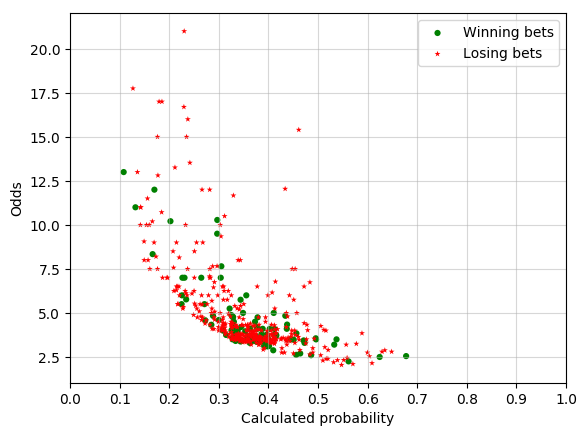
\includegraphics[width=\textwidth]{results/previous-meetings/2015-2016/odds-prob.png}
    \caption{Offered odds and predicted probabilities for the bets placed during the 2015-2016 season of the English Premier League. The probabilities are generated by the previous meetings network.}
    \label{fig:results-previous-meetings-2015-2016-odds-prob}
\end{figure}
   

\subsubsection{English Premier League 2016-2017}

\cref{fig:results-previous-meetings-2016-2017-fixed-bet,fig:results-previous-meetings-2016-2017-fixed-return,fig:results-previous-meetings-2016-2017-kelly-ratio,fig:results-previous-meetings-2016-2017-variance-adjusted} show the development of the \gls{roi} generated by the previous meetings network over the English Premier League season 2016-2017.
\begin{figure}
    \centering
    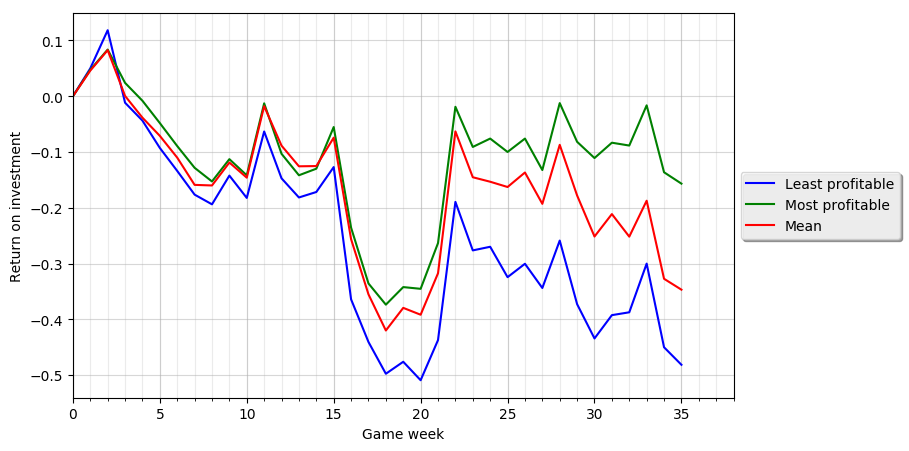
\includegraphics[width=\textwidth]{results/previous-meetings/2016-2017/fixed-bet-10.png}
    \caption{\gls{roi} over the span of the English Premier League season 2016-2017 using the previous meetings network and the fixed bet strategy.}
    \label{fig:results-previous-meetings-2016-2017-fixed-bet}
\end{figure}
\begin{figure}
    \centering
    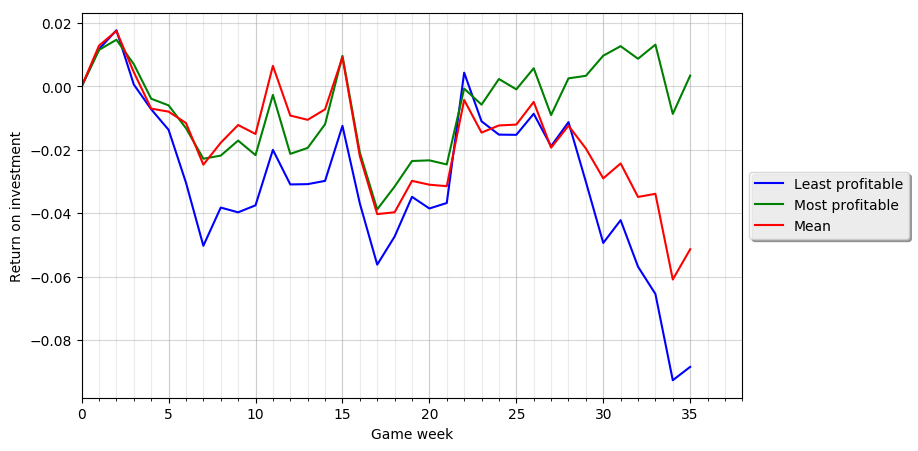
\includegraphics[width=\textwidth]{results/previous-meetings/2016-2017/fixed-return-10.png}
    \caption{\gls{roi} over the span of the English Premier League season 2016-2017 using the previous meetings network and the fixed return strategy.}
    \label{fig:results-previous-meetings-2016-2017-fixed-return}
\end{figure}
\begin{figure}
    \centering
    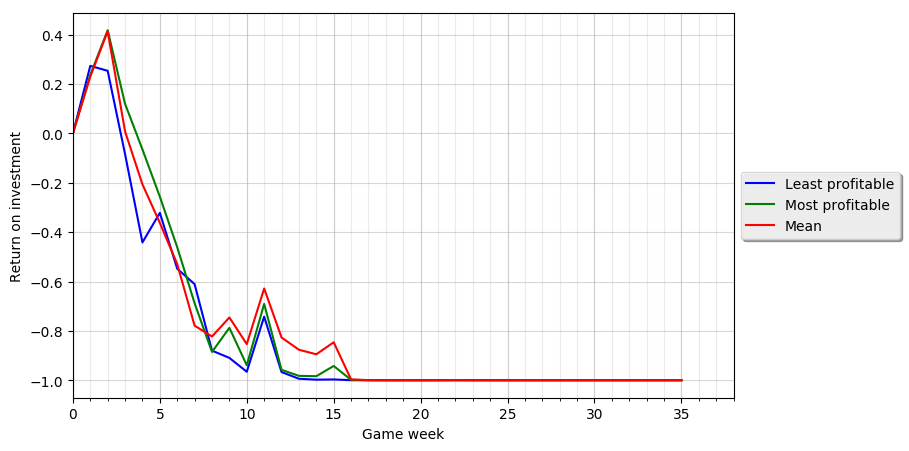
\includegraphics[width=\textwidth]{results/previous-meetings/2016-2017/kelly-ratio-10.png}
    \caption{\gls{roi} over the span of the English Premier League season 2016-2017 using the previous meetings network and the Kelly ratio strategy.}
    \label{fig:results-previous-meetings-2016-2017-kelly-ratio}
\end{figure}
\begin{figure}
    \centering
    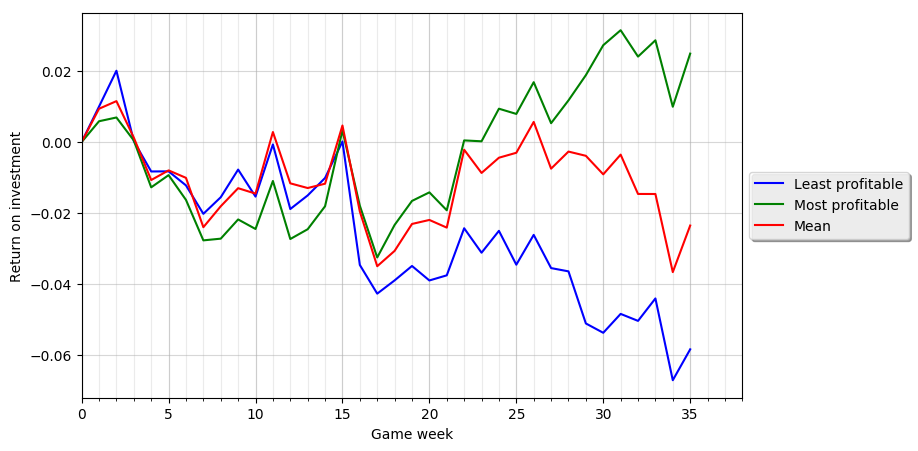
\includegraphics[width=\textwidth]{results/previous-meetings/2016-2017/variance-adjusted-10.png}
    \caption{\gls{roi} over the span of the English Premier League season 2016-2017 using the previous meetings network and the variance adjusted strategy.}
    \label{fig:results-previous-meetings-2016-2017-variance-adjusted}
\end{figure}

\cref{tab:fig:results-previous-meetings-2016-2017-roi} shows a summary of the \gls{roi} values achieved by the different strategies when used by the previous meetings network. The table shows the final \gls{roi} for the least profitable and most profitable simulations, together with the average final \gls{roi}.
\begin{table}
    \centering
    \begin{tabulary}{\textwidth}{| L || L | L | L |}
        \hline
                            & \multicolumn{3}{l |}{\textbf{Final \gls{roi}}} \\\hline
        \textbf{Strategy}   & \textbf{Min}  & \textbf{Max}  & \textbf{Mean} \\\hline
        Fixed bet           & -0.48         & -0.15         & -0.34 \\\hline
        Fixed return        & -0.09         & 0.0055        & -0.050 \\\hline
        Kelly ratio         & -1.0          & -1.0          & -1.0 \\\hline
        Variance adjusted   & -0.058        & 0.027         & \cellcolor{correct} -0.022 \\\hline
    \end{tabulary}
    \caption{Final \gls{roi} values for the four strategies when using the previous meetings network during the 2016-2017 season of the English Premier League. The green colored cell was the most profitable strategy (on average).}
    \label{tab:fig:results-previous-meetings-2016-2017-roi}
\end{table}

\cref{fig:results-previous-meetings-2016-2017-odds-prob} shows the bets placed during the 2016-2017 season of the English Premier League. The probabilities are generated by a random instance of the previous meetings network.
\begin{figure}
    \centering
    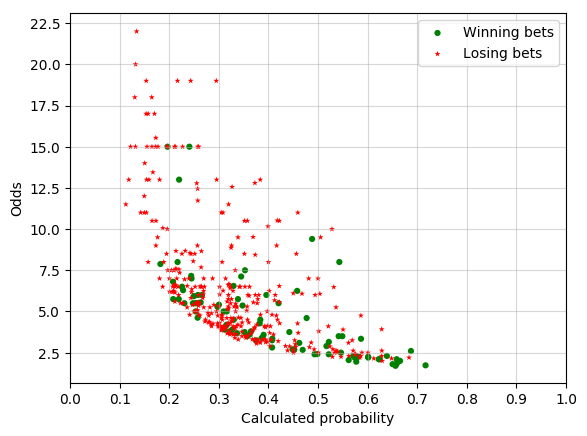
\includegraphics[width=\textwidth]{results/previous-meetings/2016-2017/odds-prob.png}
    \caption{Offered odds and predicted probabilities for the bets placed during the 2016-2017 season of the English Premier League. The probabilities are generated by the previous meetings network.}
    \label{fig:results-previous-meetings-2016-2017-odds-prob}
\end{figure}


\subsubsection{Summary}

Similarly to the head to head network, the previous meetings network did not achieve consistent good results. The first season, the fixed bet and Kelly ratio strategies performed well, gaining a profit on average. The second season, however, the same strategies achieved \glspl{roi} of -0.34 and -1.0, respectively.

\cref{fig:results-previous-meetings-2015-2016-odds-prob,fig:results-previous-meetings-2016-2017-odds-prob} show the connection between odds and probabilities predicted by the previous meetings network. The previous meetings network has a more even spread than the head to head network. However, the previous meetings network tend to overestimate the probabilities across the board. The reason for the low spread is probably the same as for the head to head network. However, the previous meetings network also utilizes team ratings, accounting for potential team changes between the seasons. Over the two seasons, the prediction models won approximately 20.3\% of all bets placed, with an average odds of 4.70.
\section{Team characteristics}

\subsection{Network structure}

\cref{tab:results-team-characteristics-accuracy} shows the \gls{rps} values and accuracy of the team characteristics network. In the evaluation data set, 41.3\% of all matches ended in a home victory.
\begin{table}
    \centering
    \begin{tabulary}{\textwidth}{| L | L || L | L | L || L |}
        \hline
        \multicolumn{2}{| l ||}{\textbf{Hidden layer}}  & \multicolumn{3}{l ||}{\textbf{\gls{rps} values}} & \\\hline
        \textbf{Activation} & \textbf{Size}             & \textbf{Min}  & \textbf{Max}  & \textbf{Mean} & \textbf{Accuracy} \\\hline
        \gls{relu}          & 32                        & 0.0143        & 0.794         & 0.226         & 0.463 \\\hline
        \gls{relu}          & 64                        & 0.00102       & 0.785         & 0.218         & 0.466 \\\hline
        \gls{relu}          & 128                       & 0.0122        & 0.719         & 0.224         & 0.458 \\\hline
        
        \hline
        
        Sigmoid             & 32                        & 0.0130        & 0.737         & 0.217         & 0.460 \\\hline
        Sigmoid             & 64                        & 0.0245        & 0.665         & 0.217         & 0.468 \\\hline
        \rowcolor{correct}
        Sigmoid             & 128*                      & 0.0169        & 0.706         & 0.213         & 0.469 \\\hline
        Sigmoid             & 256*                      & 0.0103        & 0.744         & 0.215         & 0.450 \\\hline
        
        \hline
        
        \Gls{tanh}          & 32*                       & 0.0152        & 0.775         & 0.223         & 0.445 \\\hline
        \Gls{tanh}          & 64*                       & 0.00779       & 0.800         & 0.220         & 0.461 \\\hline
        \Gls{tanh}          & 128**                     & 0.0102        & 0.698         & 0.216         & 0.463 \\\hline
        \Gls{tanh}          & 256**                     & 0.0108        & 0.823         & 0.224         & 0.461 \\\hline
    \end{tabulary}
    \caption{Accuracy of the team characteristics network, with different hidden layer configurations. The row colored green shows the configuration with most promising results.}
    \label{tab:results-team-characteristics-accuracy} 
\end{table}

Using a hidden layer with 128 nodes activated by the sigmoid function yielded the most promising results, and will therefore be used when evaluating the profitability of the team characteristics network. \cref{tab:results-team-characteristics-accuracy-2016-2017} shows the \gls{rps} values and prediction accuracy when evaluating the same configuration over the 2016-2017 season. The network achieved \gls{rps} values similar to the benchmark model the first season. The second season, the network achieved slightly better values.
\begin{table}
    \centering
    \begin{tabulary}{\textwidth}{| L | L | L || L |}
        \hline
        \multicolumn{3}{| l ||}{\textbf{\gls{rps} values}}  &                   \\\hline
        \textbf{Min}    & \textbf{Max}  & \textbf{Mean}     & \textbf{Accuracy} \\\hline
        0.0171          & 0.700         & 0.187             & 0.609             \\\hline
    \end{tabulary}
    \caption{Prediction accuracy of the team characteristics network for the 2016-2017 season of the English Premier League, using the most promising hidden layer configuration.}
    \label{tab:results-team-characteristics-accuracy-2016-2017} 
\end{table}


\subsection{Betting results}

\subsubsection{English Premier League 2015-2016}

\cref{fig:results-team-characteristics-2015-2016-fixed-bet,fig:results-team-characteristics-2015-2016-fixed-return,fig:results-team-characteristics-2015-2016-kelly-ratio,fig:results-team-characteristics-2015-2016-variance-adjusted} show the development of the \gls{roi} generated by the team characteristics network over the English Premier League season 2015-2016.
\begin{figure}
    \centering
    \includegraphics[width=\textwidth]{results/team-characteristics/2015-2016/fixed-bet-10.png}
    \caption{\gls{roi} over the span of the English Premier League season 2015-2016 using the team characteristics network and the fixed bet strategy.}
    \label{fig:results-team-characteristics-2015-2016-fixed-bet}
\end{figure}
\begin{figure}
    \centering
    \includegraphics[width=\textwidth]{results/team-characteristics/2015-2016/fixed-return-10.png}
    \caption{\gls{roi} over the span of the English Premier League season 2015-2016 using the team characteristics network and the fixed return strategy.}
    \label{fig:results-team-characteristics-2015-2016-fixed-return}
\end{figure}
\begin{figure}
    \centering
    \includegraphics[width=\textwidth]{results/team-characteristics/2015-2016/kelly-ratio-10.png}
    \caption{\gls{roi} over the span of the English Premier League season 2015-2016 using the team characteristics network and the Kelly ratio strategy.}
    \label{fig:results-team-characteristics-2015-2016-kelly-ratio}
\end{figure}
\begin{figure}
    \centering
    \includegraphics[width=\textwidth]{results/team-characteristics/2015-2016/variance-adjusted-10.png}
    \caption{\gls{roi} over the span of the English Premier League season 2015-2016 using the team characteristics network and the variance adjusted strategy.}
    \label{fig:results-team-characteristics-2015-2016-variance-adjusted}
\end{figure}

\cref{tab:fig:results-team-characteristics-2015-2016-roi} shows a summary of the \gls{roi} values achieved by the different strategies when used by the team characteristics network. The table shows the final \gls{roi} for the least profitable and most profitable simulations, together with the average final \gls{roi}.
\begin{table}
    \centering
    \begin{tabulary}{\textwidth}{| L || L | L | L |}
        \hline
                            & \multicolumn{3}{l |}{\textbf{Final \gls{roi}}} \\\hline
        \textbf{Strategy}   & \textbf{Min}  & \textbf{Max}  & \textbf{Mean} \\\hline
        Fixed bet           & 0.0010        & 0.54          & 0.21 \\\hline
        Fixed return        & -0.038        & 0.070         & -0.050 \\\hline
        Kelly ratio         & -0.25         & 2.6           &  0.80 \\\hline
        Variance adjusted   & -0.07         & 0.039         & -0.032 \\\hline
    \end{tabulary}
    \caption{Final \gls{roi} values for the four strategies when using the team characteristics network during the 2015-2016 season of the English Premier League. The green colored cell was the most profitable strategy (on average).}
    \label{tab:fig:results-team-characteristics-2015-2016-roi}
\end{table}
      
\cref{fig:results-team-characteristics-2015-2016-odds-prob} shows the bets placed during the 2015-2016 season of the English Premier League. The probabilities are generated by a random instance of the team characteristics network.
\begin{figure}
    \centering
    \includegraphics[width=\textwidth]{results/team-characteristics/2015-2016/odds-prob.png}
    \caption{Offered odds and predicted probabilities for the bets placed during the 2015-2016 season of the English Premier League. The probabilities are generated by the team characteristics network.}
    \label{fig:results-team-characteristics-2015-2016-odds-prob}
\end{figure}
  

\subsubsection{English Premier League 2016-2017}

\cref{fig:results-team-characteristics-2016-2017-fixed-bet,fig:results-team-characteristics-2016-2017-fixed-return,fig:results-team-characteristics-2016-2017-kelly-ratio,fig:results-team-characteristics-2016-2017-variance-adjusted} show the development of the \gls{roi} generated by the team characteristics network over the English Premier League season 2016-2017.
\begin{figure}
    \centering
    \includegraphics[width=\textwidth]{results/team-characteristics/2016-2017/fixed-bet-10.png}
    \caption{\gls{roi} over the span of the English Premier League season 2016-2017 using the team characteristics network and the fixed bet strategy.}
    \label{fig:results-team-characteristics-2016-2017-fixed-bet}
\end{figure}
\begin{figure}
    \centering
    \includegraphics[width=\textwidth]{results/team-characteristics/2016-2017/fixed-return-10.png}
    \caption{\gls{roi} over the span of the English Premier League season 2016-2017 using the team characteristics network and the fixed return strategy.}
    \label{fig:results-team-characteristics-2016-2017-fixed-return}
\end{figure}
\begin{figure}
    \centering
    \includegraphics[width=\textwidth]{results/team-characteristics/2016-2017/kelly-ratio-10.png}
    \caption{\gls{roi} over the span of the English Premier League season 2016-2017 using the team characteristics network and the Kelly ratio strategy.}
    \label{fig:results-team-characteristics-2016-2017-kelly-ratio}
\end{figure}
\begin{figure}
    \centering
    \includegraphics[width=\textwidth]{results/team-characteristics/2016-2017/variance-adjusted-10.png}
    \caption{\gls{roi} over the span of the English Premier League season 2016-2017 using the team characteristics network and the variance adjusted strategy.}
    \label{fig:results-team-characteristics-2016-2017-variance-adjusted}
\end{figure}

\cref{tab:fig:results-team-characteristics-2016-2017-roi} shows a summary of the \gls{roi} values achieved by the different strategies when used by the team characteristics network. The table shows the final \gls{roi} for the least profitable and most profitable simulations, together with the average final \gls{roi}.
\begin{table}
    \centering
    \begin{tabulary}{\textwidth}{| L || L | L | L |}
        \hline
                            & \multicolumn{3}{l |}{\textbf{Final \gls{roi}}} \\\hline
        \textbf{Strategy}   & \textbf{Min}  & \textbf{Max}  & \textbf{Mean} \\\hline
        Fixed bet           & -0.10         & 0.27          & 0.13 \\\hline
        Fixed return        & -0.010        & 0.14          & 0.080 \\\hline
        Kelly ratio         & -0.48         & 1.3           & \cellcolor{correct} 0.70 \\\hline
        Variance adjusted   & 0.041         & 0.21          & 0.12 \\\hline
    \end{tabulary}
    \caption{Final \gls{roi} values for the four strategies when using the team characteristics network during the 2016-2017 season of the English Premier League. The green colored cell was the most profitable strategy (on average).}
    \label{tab:fig:results-team-characteristics-2016-2017-roi}
\end{table}

\cref{fig:results-team-characteristics-2016-2017-odds-prob} shows the bets placed during the 2016-2017 season of the English Premier League. The probabilities are generated by a random instance of the team characteristics network.
\begin{figure}
    \centering
    \includegraphics[width=\textwidth]{results/team-characteristics/2016-2017/odds-prob.png}
    \caption{Offered odds and predicted probabilities for the bets placed during the 2016-2017 season of the English Premier League. The probabilities are generated by the team characteristics network.}
    \label{fig:results-team-characteristics-2016-2017-odds-prob}
\end{figure}


\subsubsection{Summary}

The team characteristics network achieved consistent good results, generating profits over both seasons using the fixed bet and Kelly ratio strategies. The network also generated profits the other strategies the first season.

\cref{fig:results-team-characteristics-2015-2016-odds-prob,fig:results-team-characteristics-2016-2017-odds-prob} show the connection between odds and probabilities predicted by the team characteristics network. The team characteristics network produce far better predictions than any other network. There is, however, a slight tendency to overestimate the probabilities in the lower fifth of the horizontal axis. Over the two seasons, the prediction models won approximately 29.4\% of all bets placed, with an average odds of 3.82.
\section{Team characteristics and strengths}

\subsection{Network structure}

\cref{tab:results-team-characteristics-and-strengths-accuracy} shows the \gls{rps} values and accuracy of the team characteristics and strengths network. In the evaluation data set, 41.5\% of all matches ended in a home victory.
\begin{table}
    \centering
    \begin{tabulary}{\textwidth}{| L | L || L | L | L || L |}
        \hline
        \multicolumn{2}{| l ||}{\textbf{Hidden layer}}  & \multicolumn{3}{l ||}{\textbf{\gls{rps} values}} & \\\hline
        \textbf{Activation} & \textbf{Size}             & \textbf{Min}  & \textbf{Max}  & \textbf{Mean} & \textbf{Accuracy} \\\hline
        \gls{relu}          & 32                        & 0.0124        & 0.761         & 0.219         & 0.434 \\\hline
        \gls{relu}          & 64*                       & 0.00991       & 0.707         & 0.215         & 0.463 \\\hline
        \gls{relu}          & 128*                      & 0.0113        & 0.728         & 0.216         & 0.459 \\\hline
        
        \hline
        
        Sigmoid             & 32                        & 0.0275        & 0.663         & 0.214         & 0.441 \\\hline
        Sigmoid             & 64                        & 0.0243        & 0.711         & 0.214         & 0.460 \\\hline
        Sigmoid             & 128                       & 0.0219        & 0.714         & 0.214         & 0.463 \\\hline
        \rowcolor{correct}
        Sigmoid             & 256*                      & 0.0146        & 0.716         & 0.213         & 0.473 \\\hline
        Sigmoid             & 512*                      & 0.0182        & 0.689         & 0.214         & 0.457 \\\hline
        
        \hline
        
        \Gls{tanh}          & 32                        & 0.00974       & 0.738         & 0.219         & 0.465 \\\hline
        \Gls{tanh}          & 64*                       & 0.00807       & 0.770         & 0.216         & 0.465 \\\hline
        \Gls{tanh}          & 128*                      & 0.0129        & 0.764         & 0.215         & 0.457 \\\hline
    \end{tabulary}
    \caption{Accuracy of the team characteristics and strengths network, with different hidden layer configurations. The row colored green shows the configuration with most promising results.}
    \label{tab:results-team-characteristics-and-strengths-accuracy} 
\end{table}

Using a hidden layer with 256 nodes activated by the sigmoid function yielded the most promising results, and will therefore be used when evaluating the profitability of the team characteristics and strengths network. \cref{tab:results-team-characteristics-and-strengths-accuracy-2016-2017} shows the \gls{rps} values and prediction accuracy when evaluating the same configuration over the 2016-2017 season. The network achieved \gls{rps} values similar to the benchmark model the first season. The second season, the network achieved slightly better values.
\begin{table}
    \centering
    \begin{tabulary}{\textwidth}{| L | L | L || L |}
        \hline
        \multicolumn{3}{| l ||}{\textbf{\gls{rps} values}}  &                   \\\hline
        \textbf{Min}    & \textbf{Max}  & \textbf{Mean}     & \textbf{Accuracy} \\\hline
        0.0139          & 0.740         & 0.184             & 0.591             \\\hline
    \end{tabulary}
    \caption{Prediction accuracy of the team characteristics to strengths network for the 2016-2017 season of the English Premier League, using the most promising hidden layer configuration.}
    \label{tab:results-team-characteristics-and-strengths-accuracy-2016-2017} 
\end{table}


\subsection{Betting results}

\subsubsection{English Premier League 2015-2016}

\cref{fig:results-team-characteristics-and-strengths-2015-2016-fixed-bet,fig:results-team-characteristics-and-strengths-2015-2016-fixed-return,fig:results-team-characteristics-and-strengths-2015-2016-kelly-ratio,fig:results-team-characteristics-and-strengths-2015-2016-variance-adjusted} show the development of the \gls{roi} generated by the team characteristics and strengths network over the English Premier League season 2015-2016.
\begin{figure}
    \centering
    \includegraphics[width=\textwidth]{results/team-characteristics-and-strengths/2015-2016/fixed-bet-10.png}
    \caption{\gls{roi} over the span of the English Premier League season 2015-2016 using the team characteristics and strengths network and the fixed bet strategy.}
    \label{fig:results-team-characteristics-and-strengths-2015-2016-fixed-bet}
\end{figure}
\begin{figure}
    \centering
    \includegraphics[width=\textwidth]{results/team-characteristics-and-strengths/2015-2016/fixed-return-10.png}
    \caption{\gls{roi} over the span of the English Premier League season 2015-2016 using the team characteristics and strengths network and the fixed return strategy.}
    \label{fig:results-team-characteristics-and-strengths-2015-2016-fixed-return}
\end{figure}
\begin{figure}
    \centering
    \includegraphics[width=\textwidth]{results/team-characteristics-and-strengths/2015-2016/kelly-ratio-10.png}
    \caption{\gls{roi} over the span of the English Premier League season 2015-2016 using the team characteristics and strengths network and the Kelly ratio strategy.}
    \label{fig:results-team-characteristics-and-strengths-2015-2016-kelly-ratio}
\end{figure}
\begin{figure}
    \centering
    \includegraphics[width=\textwidth]{results/team-characteristics-and-strengths/2015-2016/variance-adjusted-10.png}
    \caption{\gls{roi} over the span of the English Premier League season 2015-2016 using the team characteristics and strengths network and the variance adjusted strategy.}
    \label{fig:results-team-characteristics-and-strengths-2015-2016-variance-adjusted}
\end{figure}

\cref{tab:fig:results-team-characteristics-and-strengths-2015-2016-roi} shows a summary of the \gls{roi} values achieved by the different strategies when used by the team characteristics and strengths network. The table shows the final \gls{roi} for the least profitable and most profitable simulations, together with the average final \gls{roi}.
\begin{table}
    \centering
    \begin{tabulary}{\textwidth}{| L || L | L | L |}
        \hline
                            & \multicolumn{3}{l |}{\textbf{Final \gls{roi}}} \\\hline
        \textbf{Strategy}   & \textbf{Min}  & \textbf{Max}  & \textbf{Mean} \\\hline
        Fixed bet           & -0.24         & 0.28          & 0.12 \\\hline
        Fixed return        & -0.11         & 0.058         & -0.025 \\\hline
        Kelly ratio         & -1.0          & 1.3           & \cellcolor{correct} 0.49 \\\hline
        Variance adjusted   & -0.14         & 0.052         & -0.052 \\\hline
    \end{tabulary}
    \caption{Final \gls{roi} values for the four strategies when using the team characteristics and strengths network during the 2015-2016 season of the English Premier League. The green colored cell was the most profitable strategy (on average).}
    \label{tab:fig:results-team-characteristics-and-strengths-2015-2016-roi}
\end{table}
   
\cref{fig:results-team-characteristics-and-strengths-2015-2016-odds-prob} shows the bets placed during the 2015-2016 season of the English Premier League. The probabilities are generated by a random instance of the team characteristics and strengths network.
\begin{figure}
    \centering
    \includegraphics[width=\textwidth]{results/team-characteristics-and-strengths/2015-2016/odds-prob.png}
    \caption{Offered odds and predicted probabilities for the bets placed during the 2015-2016 season of the English Premier League. The probabilities are generated by the team characteristics and strengths network.}
    \label{fig:results-team-characteristics-and-strengths-2015-2016-odds-prob}
\end{figure}
     

\subsubsection{English Premier League 2016-2017}

\cref{fig:results-team-characteristics-and-strengths-2016-2017-fixed-bet,fig:results-team-characteristics-and-strengths-2016-2017-fixed-return,fig:results-team-characteristics-and-strengths-2016-2017-kelly-ratio,fig:results-team-characteristics-and-strengths-2016-2017-variance-adjusted} show the development of the \gls{roi} generated by the team characteristics and strengths network over the English Premier League season 2016-2017.
\begin{figure}
    \centering
    \includegraphics[width=\textwidth]{results/team-characteristics-and-strengths/2016-2017/fixed-bet-10.png}
    \caption{\gls{roi} over the span of the English Premier League season 2016-2017 using the team characteristics and strengths network and the fixed bet strategy.}
    \label{fig:results-team-characteristics-and-strengths-2016-2017-fixed-bet}
\end{figure}
\begin{figure}
    \centering
    \includegraphics[width=\textwidth]{results/team-characteristics-and-strengths/2016-2017/fixed-return-10.png}
    \caption{\gls{roi} over the span of the English Premier League season 2016-2017 using the team characteristics and strengths network and the fixed return strategy.}
    \label{fig:results-team-characteristics-and-strengths-2016-2017-fixed-return}
\end{figure}
\begin{figure}
    \centering
    \includegraphics[width=\textwidth]{results/team-characteristics-and-strengths/2016-2017/kelly-ratio-10.png}
    \caption{\gls{roi} over the span of the English Premier League season 2016-2017 using the team characteristics and strengths network and the Kelly ratio strategy.}
    \label{fig:results-team-characteristics-and-strengths-2016-2017-kelly-ratio}
\end{figure}
\begin{figure}
    \centering
    \includegraphics[width=\textwidth]{results/team-characteristics-and-strengths/2016-2017/variance-adjusted-10.png}
    \caption{\gls{roi} over the span of the English Premier League season 2016-2017 using the team characteristics and strengths network and the variance adjusted strategy.}
    \label{fig:results-team-characteristics-and-strengths-2016-2017-variance-adjusted}
\end{figure}

\cref{tab:fig:results-team-characteristics-and-strengths-2016-2017-roi} shows a summary of the \gls{roi} values achieved by the different strategies when used by the team characteristics and strengths network. The table shows the final \gls{roi} for the least profitable and most profitable simulations, together with the average final \gls{roi}.
\begin{table}
    \centering
    \begin{tabulary}{\textwidth}{| L || L | L | L |}
        \hline
                            & \multicolumn{3}{l |}{\textbf{Final \gls{roi}}} \\\hline
        \textbf{Strategy}   & \textbf{Min}  & \textbf{Max}  & \textbf{Mean} \\\hline
        Fixed bet           & -0.19         & 0.62          & 0.17 \\\hline
        Fixed return        & 0.016         & 0.20          & 0.080 \\\hline
        Kelly ratio         & -0.1          & 3.1           & \cellcolor{correct} 0.80 \\\hline
        Variance adjusted   & 0.045         & 0.21          & 0.13 \\\hline
    \end{tabulary}
    \caption{Final \gls{roi} values for the four strategies when using the team characteristics and strengths network during the 2016-2017 season of the English Premier League. The green colored cell was the most profitable strategy (on average).}
    \label{tab:fig:results-team-characteristics-and-strengths-2016-2017-roi}
\end{table}

\cref{fig:results-team-characteristics-and-strengths-2016-2017-odds-prob} shows the bets placed during the 2016-2017 season of the English Premier League. The probabilities are generated by a random instance of the team characteristics and strengths network.
\begin{figure}
    \centering
    \includegraphics[width=\textwidth]{results/team-characteristics-and-strengths/2016-2017/odds-prob.png}
    \caption{Offered odds and predicted probabilities for the bets placed during the 2016-2017 season of the English Premier League. The probabilities are generated by the team characteristics and strengths network.}
    \label{fig:results-team-characteristics-and-strengths-2016-2017-odds-prob}
\end{figure}


\subsubsection{Summary}

Similarly to the team characteristics network, the team characteristics network achieved consistent good results. The network generated profits over both seasons using the fixed bet and Kelly ratio strategies. The network also generated profits the other strategies the first season.

\cref{fig:results-team-characteristics-and-strengths-2015-2016-odds-prob,fig:results-team-characteristics-and-strengths-2016-2017-odds-prob} show the connection between odds and probabilities predicted by the team characteristics and strengths network. The team characteristics and strengths has the same tendency to overestimate the probabilities in the lower half as the player ratings network. This is not surprising, as the two networks share features. Over the two seasons, the prediction models won approximately 28.4\% of all bets placed, with an average odds of 3.67.
\section{Comparing the results}

\cref{tab:results-model-comparison-2015-2016,tab:results-model-comparison-2016-2017} show the average \gls{roi} for every combination of network and strategy for the two seasons.

\begin{table}
    \centering
    \begin{tabulary}{\textwidth}{| L || L |  L |  L |  L | L |  L |  L |  L |}
        \hline
        \textbf{Network}                    & \textbf{Fixed bet}        & \textbf{Fixed return}     & \textbf{Kelly ratio}      & \textbf{Variance adjusted} \\\hline
        Player ratings                      & \cellcolor{correct} 0.068 & -0.040                    & \cellcolor{correct} 0.25  & -0.073 \\\hline
        Head to head                        & \cellcolor{correct} 0.40  & \cellcolor{correct} 0.025 & \cellcolor{correct} 2.0   & -0.0080 \\\hline
        Previous meetings                   & \cellcolor{correct} 0.25  & -0.012                    & \cellcolor{correct} 1.2   & -0.052 \\\hline
        Team characteristics                & \cellcolor{correct} 0.21  & -0.050                    & \cellcolor{correct} 0.80  & -0.032 \\\hline
        Team characteristics and strengths  & \cellcolor{correct} 0.12  & -0.025                    & \cellcolor{correct} 0.49  & -0.052 \\\hline
    \end{tabulary}
    \caption{Comparison of the average \gls{roi} values for the networks. From the 2015-2016 season. Colored cells indicate profitable strategies.}
    \label{tab:results-model-comparison-2015-2016} 
\end{table}

\begin{table}
    \centering
    \begin{tabulary}{\textwidth}{| L || L |  L |  L |  L | L |  L |  L |  L |}
        \hline
        \textbf{Network}                    & \textbf{Fixed bet}        & \textbf{Fixed return}     & \textbf{Kelly ratio}      & \textbf{Variance adjusted} \\\hline
        Player ratings                      & -0.59                     & -0.095                    & -1.0                      & -0.053 \\\hline
        Head to head                        & -0.20                     & -0.018                    & -1.0                      & -0.060 \\\hline
        Previous meetings                   & -0.34                     & -0.050                    & -1.0                      & -0.022 \\\hline
        Team characteristics                & \cellcolor{correct} 0.13  & \cellcolor{correct} 0.080 & \cellcolor{correct} 0.70  & \cellcolor{correct} 0.12 \\\hline
        Team characteristics and strengths  & \cellcolor{correct} 0.17  & \cellcolor{correct} 0.080 & \cellcolor{correct} 0.80  & \cellcolor{correct} 0.13 \\\hline
    \end{tabulary}
    \caption{Comparison of the average \gls{roi} values for the networks. From the 2016-2017 season. Colored cells indicate profitable strategies.}
    \label{tab:results-model-comparison-2016-2017}
\end{table}

Only two networks were able to generate a profit over both seasons: the networks based on team characteristics. The other networks produced varying results. The head to head network generated huge profits for the first season (40\% on average using the fixed bet strategy, and 200\% on average using the Kelly ratio strategy), while suffering losses the second season (20\% on average using the fixed bet strategy, and going bankrupt for all instances using the Kelly ratio strategy).

The Kelly ratio strategy generated the highest profits, with good margin. The Kelly ratio strategy is, however, the only strategy that went bankrupt. When using the Kelly ratio strategy together with the player ratings network, all model instances were bankrupt within the eight first game weeks. The Kelly ratio strategy offers a high risk, high reward investment. The fixed return and variance adjusted strategies generated more stable results, losing at most 17\%, and no more than 10\% on average. The average profits were however not anywhere near the profits of the Kelly ratio strategy, with best average profits of 13\% and 8\%, respectively. The fixed bet strategy performed somewhere in-between the other strategies. For the worst performing networks, the fixed bet strategy suffered some huge losses. 78\% of the initial bankroll was lost when used by the player ratings network during the 2016-2017 season. For the team characteristics based networks, the fixed bet strategy performed significantly better, losing at most 25\% of the initial bankroll, with average profits of well above 10\%.
\section{Looking behind the results}

The team characteristics network achieved the best overall results over the two seasons. The first season, it was clearly the most profitable network. The second season, it was barely beaten by the team characteristics and strengths network. By analyzing the odds-probability graphs for the team characteristics network, there are some clear patterns that might help increase the profitability further.


\subsection{Placing no more than one bet per match}

\cref{tab:results-game-week-5-bets-example} shows all bets deemed feasible by a random instance of the team characteristics model during a random game week of the 2016-2017 season. Of the nine matches, a double bet was placed on four. That gives four bets that are guaranteed to fail. This pattern can be seen throughout all simulations, and is not specific for the highlighted game week alone.
\begin{table}
    \centering
    \begin{tabulary}{\textwidth}{| L | L | L | L | L |}
        \hline
        \textbf{Match}                      & \textbf{Predicted outcome}    & \textbf{Odds} & \textbf{Probability} \\\hline
        Tottenham 1 - 0 Sunderland          & A                             & 12.00         & 0.15 \\\hline
        Crystal Palace 4 - 1 Stoke          & A                             & 4.20          & 0.35 \\\hline
        Southampton 1 - 0 Swansea           & A                             & 6.17          & 0.28 \\\hline
        Watford 3 - 1 Manchester United     & H                             & 6.00          & 0.25 \\\hline
        Watford 3 - 1 Manchester United     & D                             & 4.20          & 0.28 \\\hline
        Everton 3 - 1 Middlesbrough         & A                             & 6.19          & 0.19 \\\hline
        Hull 1 - 4 Arsenal                  & H                             & 6.50          & 0.25 \\\hline
        Hull 1 - 4 Arsenal                  & D                             & 4.20          & 0.29 \\\hline
        Leicester 3 - 0 Burnley             & D                             & 4.60          & 0.27 \\\hline
        Leicester 3 - 0 Burnley             & A                             & 8.87          & 0.32 \\\hline
        Manchester City 4 - 0 Bournemouth   & D                             & 6.25          & 0.19 \\\hline
        Manchester City 4 - 0 Bournemouth   & A                             & 12.78         & 0.16 \\\hline
        Chelsea 1 - 2 Liverpool             & H                             & 2.30          & 0.54 \\\hline
    \end{tabulary}
    \caption{Bets deemed feasible by an instance of the team characteristics model. From game week 5 of the 2016-2017 season.}
    \label{tab:results-game-week-5-bets-example} 
\end{table}

To reduce the losses from placing more than one bet on a single match, one option is to only place the bet with the highest predicted probability. \cref{tab:results-single-bet-safest} shows how the average \gls{roi} values for the four strategies were affected when only placing the bet with the highest predicted probability. As the results show, only placing the "safest" bet reduced the profitability of the network.
\begin{table}
    \centering
    \begin{tabulary}{\textwidth}{| L || L | L | L | L |}
        \hline
                            & \multicolumn{2}{l |}{\textbf{2015-2016}}      & \multicolumn{2}{l |}{\textbf{2016-2017}} \\\hline
        \textbf{Strategy}   & \textbf{All feasible} & \textbf{Only best}    & \textbf{All feasible} & \textbf{Only best} \\\hline
        Fixed bet           & 0.21                  & 0.10                  & 0.13                  & 0.12 \\\hline
        Fixed return        & -0.050                & -0.051                & 0.080                 & 0.065 \\\hline
        Kelly ratio         & 0.80                  & 0.43                  & 0.70                  & 0.68 \\\hline
        Variance Adjusted   & -0.032                & -0.051                & 0.12                  & 0.090 \\\hline
    \end{tabulary}
    \caption{The effect of only allowing one bet per match. Only the bet with the highest predicted probability is placed. For the team characteristics network.}
    \label{tab:results-single-bet-safest} 
\end{table}

Another option is to only place the bet with the highest expected gain, $P_{i} * d_{i}$. \cref{tab:results-single-bet-best} shows how the average \gls{roi} values for the four strategies were affected when only placing the bet with highest expected gain. Only placing the bet with highest expected gain increased the profitability of the network slightly.
\begin{table}
    \centering
    \begin{tabulary}{\textwidth}{| L || L | L | L | L |}
        \hline
                            & \multicolumn{2}{l |}{\textbf{2015-2016}}      & \multicolumn{2}{l |}{\textbf{2016-2017}} \\\hline
        \textbf{Strategy}   & \textbf{All feasible} & \textbf{Only best}    & \textbf{All feasible} & \textbf{Only best} \\\hline
        Fixed bet           & 0.21                  & 0.22                  & 0.13                  & 0.13 \\\hline
        Fixed return        & -0.050                & -0.010                & 0.080                 & 0.085 \\\hline
        Kelly ratio         & 0.80                  & 1.0                   & 0.70                  & 0.72 \\\hline
        Variance Adjusted   & -0.032                & -0.030                & 0.12                  & 0.14 \\\hline
    \end{tabulary}
    \caption{The effect of only allowing one bet per match. Only the bet with highest expected gain is placed. For the team characteristics network.}
    \label{tab:results-single-bet-best} 
\end{table}


\subsection{Setting an odds limit}

By looking at \cref{fig:results-team-characteristics-2015-2016-odds-prob} and \cref{fig:results-team-characteristics-2016-2017-odds-prob}, one can see that hardly any bets with odds above 13 are successful. That goes for both seasons. By rejecting bets with odds above 13, the profitability of the network is increased. \cref{tab:results-odds-limit} shows how the average \gls{roi} values for the four strategies were affected. Every strategy, over both seasons, had increased profits.
\begin{table}
    \centering
    \begin{tabulary}{\textwidth}{| L || L | L | L | L |}
        \hline
                            & \multicolumn{2}{l |}{\textbf{2015-2016}}  & \multicolumn{2}{l |}{\textbf{2016-2017}} \\\hline
        \textbf{Strategy}   & \textbf{No limit} & \textbf{Max odds 13}  & \textbf{No limit} & \textbf{Max odds 13} \\\hline
        Fixed bet           & 0.21              & 0.24                  & 0.13              & 0.20 \\\hline
        Fixed return        & -0.050            & -0.030                & 0.080             & 0.11 \\\hline
        Kelly ratio         & 0.80              & 0.92                  & 0.70              & 0.9 \\\hline
        Variance Adjusted   & -0.032            & -0.028                & 0.12              & 0.13 \\\hline
    \end{tabulary}
    \caption{The effect of only allowing bets with odds less than 13. For the team characteristics network.}
    \label{tab:results-odds-limit} 
\end{table}



%========================================================================
%   CHAPTER: CONCLUSION AND FUTURE WORK
%========================================================================

\chapter{Conclusion and future work}
\label{chp:conclusion-future-work}
This chapter presents the conclusions drawn based on the results achieved in this report. The future work section presents suggestions for improvements of the prediction system.
\section{Conclusion}

This report presents a purely data-driven system for predicting football match outcomes, and for placing bets based on the predictions. The system stores large amounts of data that is easy to incorporate into the prediction model. The report shows that, even though football is a sport involving a lot of uncertainty and luck, it is possible to beat the  betting market over the span of two consecutive seasons.


\subsection{Model performance}

The results from \cref{chp:experiments-results} show that the choice of model input is crucial to the model's accuracy and profitability. When comparing the head to head network with the previous meetings network, it becomes apparent that simple assumptions sometimes are enough, and that there might be no need to build a complex network. The same goes for the team characteristics network versus the team characteristics and strengths network.

The team characteristics model performed significantly better than most models presented in \cref{sec:background-models}. Both \citet{bib:koopman-lit-2015} and \citet{bib:rue-salvesen-2000} generated profits well below the profits the team characteristics generated using the Kelly ratio strategy. However, when using the same strategies as the two other models, namely the fixed bet strategy and variance adjusted strategy, respectively, the team characteristics model did not perform as well. This highlights the importance of matching prediction model and betting strategy.

The model presented by \citet{bib:constantinou-fenton-neil-2012} performed best of the models explored in \cref{sec:background-models}. Using the same configuration: maximum odds and fixed bet strategy, the pi-football model performed significantly better than the team characteristics model (\gls{roi} of 0.83 versus 0.17). However, the team characteristics model performed better using the Kelly ratio strategy, achieving an average \gls{roi} of 0.75.


\subsection{The betting strategies}

The four betting strategies explored in this report can be compared to any other investment strategy. Strategies involving high risk have high potential gain, and at the same time higher chance of suffering losses. Strategies involving low risk have a lower probability of suffering losses, but at the same time lower potential gains. The Kelly ratio strategy is definitely the high-risk strategy, sometimes achieving impressive \gls{roi}, and sometimes going bankrupt. The fixed return strategy and variance adjusted strategy are more low-risk strategies, reducing the bet size for low-probability bets. The fixed bet strategy in an intermediate option, always placing bets of the same size. For the fixed bet, fixed return, and variance adjusted strategies to work, the prediction model needs to produce probabilities that closely match the implied probabilities of the bookmakers. The Kelly ratio strategy can to a greater extent survive on lucky strikes, generating a lot of profit.


\subsection{Applying the predictions in the betting market}

The most profitable prediction model, the team characteristics model, was able to generate an impressive average \gls{roi} of 0.75 over the two seasons using the Kelly ratio strategy. It should be noted that one instance of the network lost almost 50\% of the initial investment over one season using the same strategy. The safer strategies, fixed return and variance adjusted, achieved average \glspl{roi} of 0.015 and 0.044, respectively. The intermediate strategy, fixed bet, achieved an average \gls{roi} of 0.17, while never losing more than 10\% of the initial investment.


\subsection{Fulfillment of goal, and answering research questions}

\cref{sec:goal-research-questions} presented the goal of the report, along with two research questions stated in order to achieve the goal.

The first research question was to find out what a priori knowledge concerning a football can be fed to an \gls{ann} in order to predict the match outcome. \cref{chp:experimental-setup} presents three data sources used for predicting match outcomes: player ratings, previous meetings between the teams, and team characteristics. The data sources are used to form five different \glspl{ann}. The data sources utilized in this report are only three of many sources, but as \cref{chp:experiments-results} shows, a single data source is enough to predict the outcome of a football match with up to 60\% certainty.
    
The second research question asked how the outcome predictions can be used for generating a profit in betting. More specifically, how the choice of betting strategy affect the profitability of the network. \cref{chp:experiments-results} highlights the importance of matching prediction model and betting strategy correctly. Some combinations, as the team characteristics network and Kelly ratio strategy, can generate huge profits. Other combinations, on the other hand, as the player ratings network and fixed bet strategy, are catastrophic.

By answering the two research questions, the goal of the report has been fulfilled. The report shows that \glspl{ann} can indeed be used in order to profit from betting.

\section{Future work}

This section presents the author's suggestions for improvements of the prediction system.
\subsection{Allowing different kinds of bets}

As of now, the betting simulator only supports placing \textit{1X2} type bets (bets on a single outcome).

Throughout the experiments in this report, bets have been placed on more than one outcome for several matches. This guarantees that at least one of the bets are unsuccessful. However, the odds are usually high enough to justify the choice.

Most bookmakers offer \textit{double chance} bets. In double chance bets, one choose from three available bets, like in 1X2 bets, but with higher probabilities. The odds are, however, smaller than for single bets. The three available bets are
\begin{enumerate*}[label={\alph*)}]
    \item home victory or draw
    \item away victory or draw, and
    \item home victory or away victory.
\end{enumerate*}
Allowing double chance bets might increase the profitability of the prediction models, if the prediction model strongly suggests an outcome will \textbf{not} occur, and the odds suggest placing a double bet is better than two single bets.

Another bet type supported by most bookmakers is \textit{draw no bet}. In draw no bet type bets, the money is refunded if the match ends with a draw. This might be an alternative to the double chance bets where the predicted probability of a draw is high enough, and the draw no bet odds offered are better than the double chance odds.

Systems with good \gls{rps} values will benefit from both double chance bets and draw no bet type bets. As mentioned in \cref{sec:background-rps}, the \gls{rps} system calculates the difference between the cumulative distributions of the predicted and observed probabilities. If the observed outcome is a home victory, predicting a draw is closer to the correct outcome than what predicting an away victory is. A prediction model that achieves good \gls{rps} values is therefore probably good at knowing what the final outcome will \textbf{not} be. This can be exploited if the corresponding double chance odds are high enough. Draw no bet type bets will be beneficial if the model overestimates the probability of drawn matches.
\subsection{Considering betting biases}

As mentioned in \cref{subsec:background-betting-biases}, bookmakers are biased. As of now, the betting simulator treats all bets equally, without taking any kind of bias into account.

To take the favorite-longshot into account, one can add a confidence threshold that increases with the odds. The same can be done with the predicted probability for the most-likely/least-likely bias. For the home-away bias, the required confidence needed to place a bet can be higher for away victories.
\subsection{Include more bookmakers}

As of now, the betting simulator only considers odds offered by seven bookmakers. This was mostly done for simplicity, as the historical match data presented at \citet{bib:football-data} only contains 1X2 odds from seven bookmakers. The data from \citet{bib:football-data} was used as it is neatly stored in CSV files, and can easily be fetched without scraping any web page.

In the future, one should look into other web sites offering odds history, such as \citet{bib:odds-portal}. \citet{bib:odds-portal} shows odds from more than 50 bookmakers (as of June 2017). For the match between Arsenal and Manchester United May 7, 2017, the \citet{bib:odds-portal} present odds from 55 bookmakers. The average odds offered were 2.09, 3.49, and 3.56 for home victory, draw, and away victory, respectively, whilst the highest odds were 2.16, 3.64, and 3.72.


\subsubsection{Exploiting arbitrage opportunities}

A way of securing extra profits is to exploit arbitrage opportunities. Arbitrage opportunities occur when the odds offered by different bookmakers vary enough to guarantee a profit. This method might go a bit beyond the scope of this report, as is does not require any prediction model. Nonetheless, it can still be used to increase the profitability of the system.

For the match between Arsenal and Everton May 21, 2017, the maximum available odds were 1.42, 6.20, 9.80, for home victory, draw, and away victory, respectively. The expected gain of the betting market was $\frac{1}{1.42} + \frac{1}{6.20} + \frac{1}{9.80} - 1 = -0,032$. The betting market was expected to suffer losses of $3.2\%$.

If the betting marked is expected to suffer losses, arbitrage is possible. \cref{alg:arbitrage-procedure} shows how to secure profits from arbitrage.
\begin{algorithm}
    \caption{How to secure profits from arbitrage \label{alg:arbitrage-procedure}}
    set desired total winnings, $C$\;
    \For{outcome $i \in \{0, 1, 2\}$}{
        place bet of size $C / d_{i}$ on outcome $i$
    }
\end{algorithm}

\cref{tab:future-work-arbitrage-example} shows how one could guarantee a profit for the match between Arsenal and Everton May 21, 2017. The desired total winnings, $C$, is set to 100 units.
\begin{table}
    \centering
    \begin{tabulary}{\textwidth}{| L | L | L | L |}
        \hline
                            & \textbf{Home victory} & \textbf{Draw}             & \textbf{Away victory} \\\hline
        Best odds           & 1.42                  & 6.20                      & 9.80                  \\\hline
        Stake               & $100 / 1.42 = 70.42$  & $100 / 6.20 = 16.13$      & $100 / 9.80 = 10.20$  \\\hline
        Profit if win       & 29.58                 & 83.88                     & 90.16                 \\\hline
        Lost stakes         & 26.33                 & 80.62                     & 86.55                 \\\hline
        Total profit if win & 3.25                  & 3.25                      & 3.61                  \\\hline
    \end{tabulary}
    \caption{How to guarantee a profit for the match between Arsenal and Everton May 21, 2017.}
    \label{tab:future-work-arbitrage-example} 
\end{table}
\subsection{Explore the impact of other available data}

The prediction models constructed for this report utilizes three data sources: player ratings, previous meetings between the teams, and team characteristics. For future development of the prediction models, further exploring the data available at \whoscored\ is a good start.

\cref{subsec:variables-team-characteristics} presents interesting analyses of team characteristics. \citet{bib:bialkowski-lucey-carr-yue-sridharan-matthews-2014} mention how they in the future plan on using their findings for match outcome prediction. It would be interesting to explore the predictive properties the data from \cref{fig:bialkowski-et-al-ball-occupancy} or \cref{fig:bialkowski-et-al-formation-descriptors}. Exploring the predictive properties of the "significance" of different matches, as mentioned by \citet{bib:goddard-asimakopoulos-2004}, would also be interesting.

The team characteristics used in this report are all generated by the match events at \whoscored. It would be interesting check if the events themselves hold better predicative information. By using the events themselves, the middle man is cut out. The underlying events might contain more predictive information than the aggregated characteristics.


%========================================================================
%   BIBLIOGRAPHY
%========================================================================

\printbibliography[heading=bibintoc, title={References}]


%========================================================================
%   APPENDICES
%========================================================================

% Rename chapter to appendix
\renewcommand\chaptername{Appendix}

\begin{appendices}
    \crefalias{chapter}{appendix}\chapter{Results from previous models}

\section{\citet{bib:maher-1982}}

\begin{figure}
    \centering
    \includegraphics[width=\textwidth]{old-results/maher-strengths.png}
    \caption{Maximum likelihood estimates of the parameters for the English Division 1 1971-1972. Taken from \citet{bib:maher-1982}.}
    \label{fig:app-maher-strengths}
\end{figure}

\begin{figure}
    \centering
    \includegraphics[width=\textwidth]{old-results/maher-double-frequencies.png}
    \caption{Comparison of expected and observed number of goals scored for home and away teams for the English Division 1 1971-1972. Taken from \citet{bib:maher-1982}.}
    \label{fig:app-maher-double-frequencies}
\end{figure}

\begin{figure}
    \centering
    \includegraphics[width=\textwidth]{old-results/maher-bivariate-frequencies.png}
    \caption{Observed and estimated frequencies for Z, the goal difference, for the English Division 1 1971-1972 using different values for $\varrho$. Taken from \citet{bib:maher-1982}.}
    \label{fig:app-maher-bivariate-frequencies}
\end{figure}


\section{\citet{bib:karlis-ntzoufras-2003}}

\begin{figure}
    \centering
    \includegraphics[width=\textwidth]{old-results/karlis-ntzoufras-2003-results.png}
    \caption{The estimates by different versions of the model from \citet{bib:karlis-ntzoufras-2003}. Taken from \citet{bib:karlis-ntzoufras-2003}.}
    \label{fig:app-karlis-ntzoufras-2003-results}
\end{figure}


\section{\citet{bib:koopman-lit-2015}}

\begin{figure}
    \centering
    \includegraphics[width=\textwidth]{old-results/koopman-lit-threshold-levels.png}
    \caption[Average return from \citet{bib:koopman-lit-2015}.]{
        \begin{enumerate*}[label={(\roman*)}]
            \item The average return from betting on match outcomes in the English Premier League 2010-2012 using different values for $\tau$. Plotted together with $90\%$ bootstrap confidence intervals.
            \item The number of feasible bets for different values of $\tau$.
        \end{enumerate*} Taken from \citet{bib:koopman-lit-2015}
    }
    \label{fig:app-koopman-lit-threshold-levels}
\end{figure}


\section{\citet{bib:rue-salvesen-2000}}

\begin{figure}
    \centering
    \includegraphics[width=0.8\textwidth]{old-results/rue-salvesen-profits.png}
    \caption{The observed profit in the simulated betting experiments for the English Premier League and Division 1 1997-1998. Taken from \citet{bib:rue-salvesen-2000}.}
    \label{fig:app-rue-salvesen-profits}
\end{figure}


\section{\citet{bib:hvattum-arntzen-2010}}

\begin{figure}
    \centering
    \includegraphics[width=\textwidth]{old-results/hvattum-arntzen-2010-profits.png}
    \caption{Average bet size (BS) and total return on bets (TROB) based on simulated betting on 14,927 matches from the English league system, using seven different betting strategies. Here, UNIT BET represents Fixed bet, UNIT WIN Fixed return, and KELLY the Kelly ratio strategy. Taken from \citet{bib:hvattum-arntzen-2010}.}
    \label{fig:app-hvattum-arntzen-2010-profits}
\end{figure}


\section{\citet{bib:constantinou-fenton-neil-2012}}

\begin{figure}
    \centering
    \includegraphics[width=\textwidth]{old-results/constantinou-fenton-neil-2012-profits.png}
    \caption{Cumulative profits observed when simulating the Unit bet strategy at discrepancy levels of $\geq 5\%$ against (a) $f_{maxB}$, (b) $f_{meanB}$, and (c) $f_{WH}$. Taken from \citet{bib:constantinou-fenton-neil-2012}.}
    \label{fig:app-constantinou-fenton-neil-2012-profits}
\end{figure}

\begin{figure}
    \centering
    \includegraphics[width=\textwidth]{old-results/constantinou-fenton-neil-2012-bets.png}
    \caption{Betting simulation stats against (a) $f_{maxB}$, (b) $f_{meanB}$, and (c) $f_{WH}$ at discrepancy levels of $\geq 5\%$. Taken from \citet{bib:constantinou-fenton-neil-2012}.}
    \label{fig:app-constantinou-fenton-neil-2012-bets}
\end{figure}
    \crefalias{chapter}{appendix}\chapter{\whoscoredplain\ data}
\label{chp:whoscored-data-description}


\section{Match events}

\begin{table}
    \centering
    \noindent\begin{tabulary}{\textwidth}{| L | L |}
        \hline
        \textbf{Name}       & \textbf{Description} \\\hline
        Start               & The match started \\\hline
        End                 & The match ended \\\hline
        Formation set       & Initial formation information for a team \\\hline
        
        Corner awarded      & A team was awarded a corner \\\hline
        Offside provoked    & A team was caught offside \\\hline
        Formation change    & A team made a change in their formation \\\hline
        Turnover            & A team made a turnover \\\hline
        Cross not claimed   & A cross was not claimed by the team \\\hline
        Shield ball opp     & The opposing team shielded the ball \\\hline
        
        Save                & A keeper made a save \\\hline
        Saved shot          & A keeper saved a shot \\\hline
        Penalty faced       & A keeper faced a penalty \\\hline
        Keeper sweeper      & A keeper swept the ball \\\hline
        Claim               & A keeper claimed the ball \\\hline
        Punch               & A keeper punched the ball \\\hline
        Smother             & A keeper made a smother save \\\hline
        Keeper pickup       & A keeper picked up the ball \\\hline
        
        Pass                & A player made a pass \\\hline
        Goal                & A player scored a goal \\\hline
        Ball recovery       & A player recovered the ball from the opposing team \\\hline
        Ball touch          & A player made a touch on the ball \\\hline
        Take on             & A player took on another player \\\hline
        Tackle              & A player made a tackle \\\hline
        Dispossessed        & A player lost possession of the ball \\\hline
        Interception        & A player intercepted a pass \\\hline
        Clearance           & A player made a clearance \\\hline
        Blocked pass        & A player blocked a pass \\\hline
        Aerial              & A player went into an aerial duel \\\hline
        Foul                & A player made a foul \\\hline
        Missed shots        & A player missed a shot \\\hline
        Challenge           & A player challenged another player for the ball \\\hline
        Card                & A player was awarded a card \\\hline
        Error               & A player made en error \\\hline
        Substitution off    & A player was substituted off \\\hline
        Substitution on     & A player was substituted on \\\hline
        Shot on post        & A player hit a goal post with a shot \\\hline
        Good skill          & A player showed good skills \\\hline
        Chance missed       & A player missed a chance \\\hline
        Offside pass        & A pass offside provoking was made \\\hline
    \end{tabulary}
    \caption{Different event types in the detailed matches at \whoscored.}
    \label{tab:whoscored-event-types}
\end{table}

\begin{table}
    \centering
    \noindent\begin{tabulary}{\textwidth}{| L | L | L | L |}
        \hline
        \textbf{Name}       & \textbf{Description}                                              & \textbf{Mandatory?} \\\hline
        ID                  & Unique event ID                                                   & \xmark \\\hline
        Event ID            & ID relative to the match                                          & \xmark \\\hline
        Minute              & What minute the event occurs                                      & \cmark \\\hline
        Second              & What second the event occurs                                      & \cmark \\\hline
        Player ID           & ID of the player the event concerns                               & \xmark \\\hline
        Related player ID   & ID of other player the event concerns                             & \xmark \\\hline
        X                   & X coordinate of where the event occurs                            & \xmark \\\hline
        Y                   & Y coordinate of where the event occurs                            & \xmark \\\hline
        End x               & X coordinate of where the event ends                              & \xmark \\\hline
        End y               & Y coordinate of where the event ends                              & \xmark \\\hline
        Goal mouth x        & X coordinate of where the ball entered the goal                   & \xmark \\\hline
        Goal mouth y        & Y coordinate of where the ball entered the goal                   & \xmark \\\hline
        Period              & What match half the event occurs                                  & \xmark \\\hline
        Type                & What type of event it is (\cref{tab:whoscored-event-types})       & \xmark \\\hline
        Outcome             & Whether the event is successful or unsuccessful                   & \xmark \\\hline
        Qualifiers          & List of different event properties                                & \cmark \\\hline
        Is touch            & Whether event is a touch                                          & \xmark \\\hline
        Is goal             & Whether event is a goal                                           & \xmark \\\hline
        Is own goal         & Whether event is an own goal                                      & \xmark \\\hline
        Is penalty          & Whether event is a penalty                                        & \xmark \\\hline
        Is touch            & Whether event is a touch                                          & \xmark \\\hline
    \end{tabulary}
    \caption{Properties of a detailed event at \whoscored.}
    \label{tab:whoscored-event-properties}
\end{table}


\section{Player metrics}

\begin{table}
    \centering
    \noindent\begin{tabulary}{\textwidth}{| L | L |}
        \hline
        \textbf{Name}           & \textbf{Description} \\\hline
        Tackles successful      & Number of successful tackles \\\hline
        Tackles unsuccessful    & Number of unsuccessful tackles \\\hline
        Tackles total           & Total number of tackles \\\hline
        
        Shots on target         & Number of shots on target \\\hline
        Shots off target        & Number of shots off target \\\hline
        Shots blocked           & Number of shots blocked \\\hline
        Shots on post           & Number of shots to hit a goal post \\\hline
        Shots total             & Total number of shots \\\hline
        
        Dribbles won            & Number of dribbles won \\\hline
        Dribbles lost           & Number of dribbles lost \\\hline
        Dribbles attempted      & Total number of dribbles attempted \\\hline
        Dribbled past           & Number of times the player was dribbled past \\\hline
        
        Passes accurate         & Number of accurate passes \\\hline
        Passes key              & Number of key passes \\\hline
        Passes total            & Total number of passes \\\hline
        
        Touches                 & Number of touches \\\hline
        Possessions             & Number of times the player was in possession of the ball \\\hline
        
        Interceptions           & Number of interceptions made \\\hline
        Fouls committed         & Number of fouls committed \\\hline
        Claims high             & Number of claims made high on the pitch \\\hline
        Clearances              & Number of clearances made \\\hline
        Parried safe            & Number of times the player successfully parried the ball \\\hline
        Parried danger          & Number of times the player parried the ball into a dangerous situation \\\hline
        Errors                  & Number of errors made \\\hline
        
        Dispossessed            & Number of times the player lost the ball \\\hline
        Offsides caught         & Number of times the player was caught offside \\\hline
        Corners accurate        & Number of accurate corners kicked \\\hline
        Corners total           & Total number of corners kicked \\\hline
        
        Collected               & Number of times the player collected the ball \\\hline
        Total saves             & Total number of saves made \\\hline
        
        Offensive aerials       & Number of offensive aerials participated in \\\hline
        Defensive aerials       & Number of defensive aerials participated in \\\hline
        Aerials won             & Number of aerials won \\\hline
        Aerials total           & Total number of aerials \\\hline
    \end{tabulary}
    \caption{List of player metrics in the detailed matches at \whoscored.}
    \label{tab:whoscored-player-metrics}
\end{table}


\section{Views}

\begin{table}
    \centering
    \noindent\begin{tabular}{| p{3cm} | p{10cm} |}
        \hline
        \textbf{URL post-fix} & \textbf{Description} \\\hline
        Preview & Probable lineups, missing players, and top players. \\\hline
        Show & Last matches between the competing teams. Current table positions (if applicable). Last matches for the competing teams. Team characteristics at the time of the match. \\\hline
        TeamStatistics & Team characteristics at the time of the match (the same as in the \url{Live} view). Per-match statistics, listing average number of goals, shots, cards, corners, fouls, etc. for the competing teams. Situational statistics, listing summary of goals for/against the teams, passing history, and cards history. Positional statistics, highlighting where on the pitch the teams usually play and shoot. \\\hline
        PlayerStatistics & Height, weight, matches played, minutes played, ratings, and numbers from \cref{tab:whoscored-player-metrics} for the players in the competing teams' squads. \\\hline
        Betting & Odds (if match is not finished). Summary of the teams' recent results. Summary of goals scored by the teams (how many, scoring times, and number of clean sheets and goal-less games). \\\hline
        Live & "Match Centre": overview of the players, with their positions, substitutions, final ratings, and most important events. "Match Commentary": timeline containing textual descriptions of how the match progressed. "Chalkboard": spatiotemporal overview over player events (shots, passes, dribbles, clearances, saves, etc.). "Heatmaps": heatmaps, highlighting where on the pitch the different players contributed to the match. "Live Stream": live stream of the match (if available) \\\hline
        MatchReport & Textual summary of the teams' strengths, weaknesses, and styles. Situational report, listing the number of attempts, passes, and card situations. \\\hline
        LiveStream & Live stream of the match (if available). \\\hline
    \end{tabular}
    \caption{List of different views for matches at \whoscored.}
    \label{tab:whoscored-match-views}
\end{table}

\begin{table}
    \centering
    \noindent\begin{tabular}{| p{3cm} | p{10cm} |}
        \hline
        \textbf{URL post-fix} & \textbf{Description} \\\hline
        Show & List of recent matches. List of coming matches. Current squad, with summary of the numbers from \cref{tab:whoscored-player-metrics} for each player. Team characteristics. Top players. Formation summary (seasonal, last match, and a list of what positions the current squad members have played). \\\hline
        Fixtures & List of the team's matches the current season. \\\hline
        Statistics & Match statistics (average number of cards, possession, passes, shots, tackles, etc.). Situational statistics (where the team usually scores from, what kind of passes are usually made, and how the team is usually awarded cards). Positional statistics, including where on the pitch the team usually plays and where on the pitch the team usually shoot for the goal. \\\hline
        RefereeStatistics & List of all referees that have conducted the team, including number of matches the have conducted, cards they have issued, and penalties they have awarded. \\\hline
        History & List of team squads, with summary of the numbers from \cref{tab:whoscored-player-metrics} for each player. Option show statistics from different seasons. \\\hline
    \end{tabular}
    \caption{List of different views for teams at \whoscored.}
    \label{tab:whoscored-team-views}
\end{table}

\begin{table}
    \centering
    \noindent\begin{tabular}{| p{3cm} | p{10cm} |}
        \hline
        \textbf{URL post-fix} & \textbf{Description} \\\hline
        Show & Player information (name, height, weight, full name, age, nationality, current team, shirt number, positions). Tournaments the player currently participates in, with summary of the numbers from \cref{tab:whoscored-player-metrics}. List of different playing positions the player has had. Player characteristics. List of the last 10 matches the player participated in. \\\hline
        Fixtures & List of matches the current season where the player has participated. \\\hline
        History & Summary of the player's career, including competitions, matches played, minutes played, and the numbers from \cref{tab:whoscored-player-metrics} \\\hline
    \end{tabular}
    \caption{List of different views for players at \whoscored.}
    \label{tab:whoscored-player-views}
\end{table}


\section{Match header}

\begin{table}
    \centering
    \noindent\begin{tabular}{| l |}
        \hline
        \textbf{Description} \\\hline
        Home team ID \\\hline
        Away team ID \\\hline
        Home team name \\\hline
        Away team name \\\hline
        Kickoff time \\\hline
        Start of match date \\\hline
        Match status \\\hline
        Elapsed time (HT for half time, FT for full time, EAT for extra after time, PEN for after penalties) \\\hline
        Half time score \\\hline
        Full time score \\\hline
        Score after extra time \\\hline
        Score after penalties \\\hline
        Final score \\\hline
        Home team country \\\hline
        Away team country \\\hline
    \end{tabular}
    \caption{Ordered list of fields in \whoscored\ match header.}
    \label{tab:whoscored-match-header-data}
\end{table}
\end{appendices}


\end{document}